%% LyX 2.3.6.1 created this file.  For more info, see http://www.lyx.org/.
%% Do not edit unless you really know what you are doing.
%\documentclass[11pt,american,czech]{book}
\documentclass[11pt,oneside,american,czech]{book}
\usepackage[T1]{fontenc}
\usepackage[utf8]{inputenc}
\usepackage[a4paper]{geometry}
\geometry{verbose,tmargin=4cm,bmargin=3cm,lmargin=3cm,rmargin=2cm,headheight=0.8cm,headsep=1cm,footskip=0.5cm}
\pagestyle{headings}
\setcounter{secnumdepth}{3}
\usepackage{url}
\usepackage{mathtools}
\usepackage{amsmath}
\usepackage{amsthm}
\usepackage{amssymb}
\usepackage{empheq} 
\usepackage{graphicx}
\usepackage{setspace}
\usepackage{siunitx}
\usepackage{multicol}
\usepackage{subcaption}
\usepackage[hidelinks]{hyperref}
\usepackage{float}
\usepackage{booktabs}
\usepackage{tabularx}
\usepackage[svgnames]{xcolor}
\usepackage[most]{tcolorbox}
\usepackage{listings}
\usepackage[draft]{todonotes}
\usepackage{colortbl}
\usepackage[toc, page]{appendix}
\usepackage{multirow}


\renewcommand\appendixpagename{Přílohy}
\renewcommand\appendixtocname{Přílohy}

\DeclareCaptionLabelFormat{andtable}{#1~#2  \&  \tablename~\thetable}

\definecolor{codegreen}{rgb}{0,0.6,0}
\definecolor{codegray}{rgb}{0.5,0.5,0.5}
\definecolor{codepurple}{rgb}{0.58,0,0.82}
\definecolor{backcolour}{rgb}{0.95,0.95,0.92}

\lstdefinestyle{mystyle}{
	backgroundcolor=\color{backcolour},   
	commentstyle=\color{codegreen},
	keywordstyle=\color{magenta},
	numberstyle=\tiny\color{codegray},
	stringstyle=\color{codepurple},
	basicstyle=\ttfamily\footnotesize,
	breakatwhitespace=false,         
	breaklines=true,                 
	captionpos=b,                    
	keepspaces=true,                 
	numbers=left,                    
	numbersep=5pt,                  
	showspaces=false,                
	showstringspaces=false,
	showtabs=false,                  
	tabsize=2
}
\lstset{style=mystyle}

\lstset{
	literate={š}{{s}}1
	{ä}{{\"a}}1
	{ü}{{\"u}}1
}


\usepackage{ upgreek }
\tcbuselibrary{skins,breakable}
\usetikzlibrary{shadings,shadows}

\hypersetup{
	colorlinks,
	linkcolor={red},
	citecolor={blue},
	urlcolor={purple}
}

%
%\hypersetup{
%	colorlinks,
%	linkcolor={black},
%	citecolor={black},
%	urlcolor={black}
%}

\definecolor{myGrey}{rgb}{0.55, 0.55, 0.55}


\newcommand\norm[1]{\left\lVert#1\right\rVert}
\newcommand*\widefbox[1]{\fbox{\hspace{2em}#1\hspace{2em}}}
\makeatletter
\newcommand\bb[1]{{\left(#1\right)}}
%%%%%%%%%%%%%%%%%%%%%%%%%%%%%% Textclass specific LaTeX commands.
\newenvironment{lyxlist}[1]
	{\begin{list}{}
		{\settowidth{\labelwidth}{#1}
		 \setlength{\leftmargin}{\labelwidth}
		 \addtolength{\leftmargin}{\labelsep}
		 \renewcommand{\makelabel}[1]{##1\hfil}}}
	{\end{list}}

%%%%%%%%%%%%%%%%%%%%%%%%%%%%%% User specified LaTeX commands.
%% Font setup: please leave the LyX font settings all set to 'default'
%% if you want to use any of these packages:

%% Use Times New Roman font for text and Belleek font for math
%% Please make sure that the 'esint' package is turned off in the
%% 'Math options' page.
\usepackage[varg]{txfonts}
\usepackage{pdfpages}

%% Use Utopia text with Fourier-GUTenberg math
%\usepackage{fourier}

%% Bitstream Charter text with Math Design math
%\usepackage[charter]{mathdesign}
%\usepackage[varg]{mathdesign}

%%---------------------------------------------------------------------

%% Make the multiline figure/table captions indent so that the second
%% line "hangs" right below the first one.
%\usepackage[format=hang]{caption}

%% Indent even the first paragraph in each section
\usepackage{indentfirst}

%%---------------------------------------------------------------------

%% Disable page numbers in the TOC. LOF, LOT (TOC automatically
%% adds \thispagestyle{chapter} if not overriden
%\addtocontents{toc}{\protect\thispagestyle{empty}}
%\addtocontents{lof}{\protect\thispagestyle{empty}}
%\addtocontents{lot}{\protect\thispagestyle{empty}}

%% Shifts the top line of the TOC (not the title) 1cm upwards 
%% so that the whole TOC fits on 1 page. Additional page size
%% adjustment is performed at the point where the TOC
%% is inserted.
%\addtocontents{toc}{\protect\vspace{-1cm}}


\newtcolorbox[auto counter,number within=chapter]{uloha}[2][]{
	enhanced,
	colframe = myGrey,
%	colback  = #2!10,
%	coltitle = #2!20!black,
	breakable,
	arc=0pt,
	outer arc=0pt,
	boxrule=0.9pt,
	rightrule=0.9pt,
	bottomrule=0.9pt,
	fonttitle=\scshape,
	title={\textbf{{\large Úloha}} {\large \thetcbcounter: \hspace{0.1mm}} {\large #2}}
}
%%---------------------------------------------------------------------

% completely avoid orphans (first lines of a new paragraph on the bottom of a page)
\clubpenalty=9500

% completely avoid widows (last lines of paragraph on a new page)
\widowpenalty=9500

% disable hyphenation of acronyms
\hyphenation{CDFA HARDI HiPPIES IKEM InterTrack MEGIDDO MIMD MPFA DICOM ASCLEPIOS MedInria}

%%---------------------------------------------------------------------

%% Print out all vectors in bold type instead of printing an arrow above them
\renewcommand{\vec}[1]{\boldsymbol{#1}}
\renewcommand{\lstlistingname}{Příklad kódu}

% Replace standard \cite by the parenthetical variant \citep
%\renewcommand{\cite}{\citep}

\makeatother

\usepackage[czech]{babel}
\begin{document}

\def\documentdate{21. kv\v{e}tna 2023}

%%\def\documentdate{\today}

\pagestyle{empty}
{\centering

\noindent %
\begin{minipage}[c]{3cm}%
\noindent \begin{center}

\includegraphics[width=3cm,height=3cm,keepaspectratio]{Images/TITLE/cvut}
\par\end{center}%
\end{minipage}%
\begin{minipage}[c]{0.6\linewidth}%
\begin{center}
\textsc{\large{}České vysoké učení technické v Praze}{\large{}}\\
{\large{}Fakulta jaderná a fyzikálně inženýrská}
\par\end{center}%
\end{minipage}%
\begin{minipage}[c]{3cm}%
\noindent \begin{center}

\includegraphics[width=3cm,height=3cm,keepaspectratio]{Images/TITLE/fjfi}
\par\end{center}%
\end{minipage}

\vspace{3cm}

\textbf{\huge{}Hledání optimálního tvaru stěn matematického modelu proudění krve v problematice úplného kavopulmonálního cévního napojení}{\huge\par}

\vspace{1cm}

\selectlanguage{american}%
\textbf{\huge{}Optimal shape design of walls of blood flow mathematical model focusing on the total cavopulmonary connection}{\huge\par}

\selectlanguage{czech}%
\vspace{2cm}

{\large{}Výzkumný úkol}{\large\par}
\vfill{}

\begin{lyxlist}{MMMMMMMMM}
	\begin{singlespace}
		\item [{Autor:}] \textbf{Bc. Jan Bureš}
		\item [{Vedoucí~práce:}] \textbf{doc. Ing. Radek Fučík, Ph.D.}
		\item [{Konzultant:}] \textbf{Ing. Pavel Eichler}
		\item [{Akademický~rok:}] 2022/2023
	\end{singlespace}
\end{lyxlist}
\newpage{}
}



~\newpage{}

~

\vfill{}

%\def\documentdate{21. kv\v{e}tna 2023}

%%\def\documentdate{\today}

\pagestyle{empty}
{\centering

\noindent %
\begin{minipage}[c]{3cm}%
\noindent \begin{center}

\includegraphics[width=3cm,height=3cm,keepaspectratio]{Images/TITLE/cvut}
\par\end{center}%
\end{minipage}%
\begin{minipage}[c]{0.6\linewidth}%
\begin{center}
\textsc{\large{}České vysoké učení technické v Praze}{\large{}}\\
{\large{}Fakulta jaderná a fyzikálně inženýrská}
\par\end{center}%
\end{minipage}%
\begin{minipage}[c]{3cm}%
\noindent \begin{center}

\includegraphics[width=3cm,height=3cm,keepaspectratio]{Images/TITLE/fjfi}
\par\end{center}%
\end{minipage}

\vspace{3cm}

\textbf{\huge{}Hledání optimálního tvaru stěn matematického modelu proudění krve v problematice úplného kavopulmonálního cévního napojení}{\huge\par}

\vspace{1cm}

\selectlanguage{american}%
\textbf{\huge{}Optimal shape design of walls of blood flow mathematical model focusing on the total cavopulmonary connection}{\huge\par}

\selectlanguage{czech}%
\vspace{2cm}

{\large{}Soutěžní práce\\Rektorysova soutěž 2023}{\large\par}
\vfill{}

\begin{lyxlist}{MMMMMMMMM}
	\begin{singlespace}
		\item [{Autor:}] \textbf{Bc. Jan Bureš}
		\item [{Vedoucí~práce:}] \textbf{doc. Ing. Radek Fučík, Ph.D.}
		\item [{Konzultant:}] \textbf{Ing. Pavel Eichler, Ph.D.}
		\item [{Akademický~rok:}] 2022/2023
	\end{singlespace}
\end{lyxlist}
\newpage{}
}


%%\begin{center}
%- Zadání práce -
%\par\end{center}
%
%\vfill{}
%
%~\newpage{}
%
%~
%
%\vfill{}
%
%\begin{center}
%- Zadání práce (zadní strana) -
%\par\end{center}
%
%\vfill{}
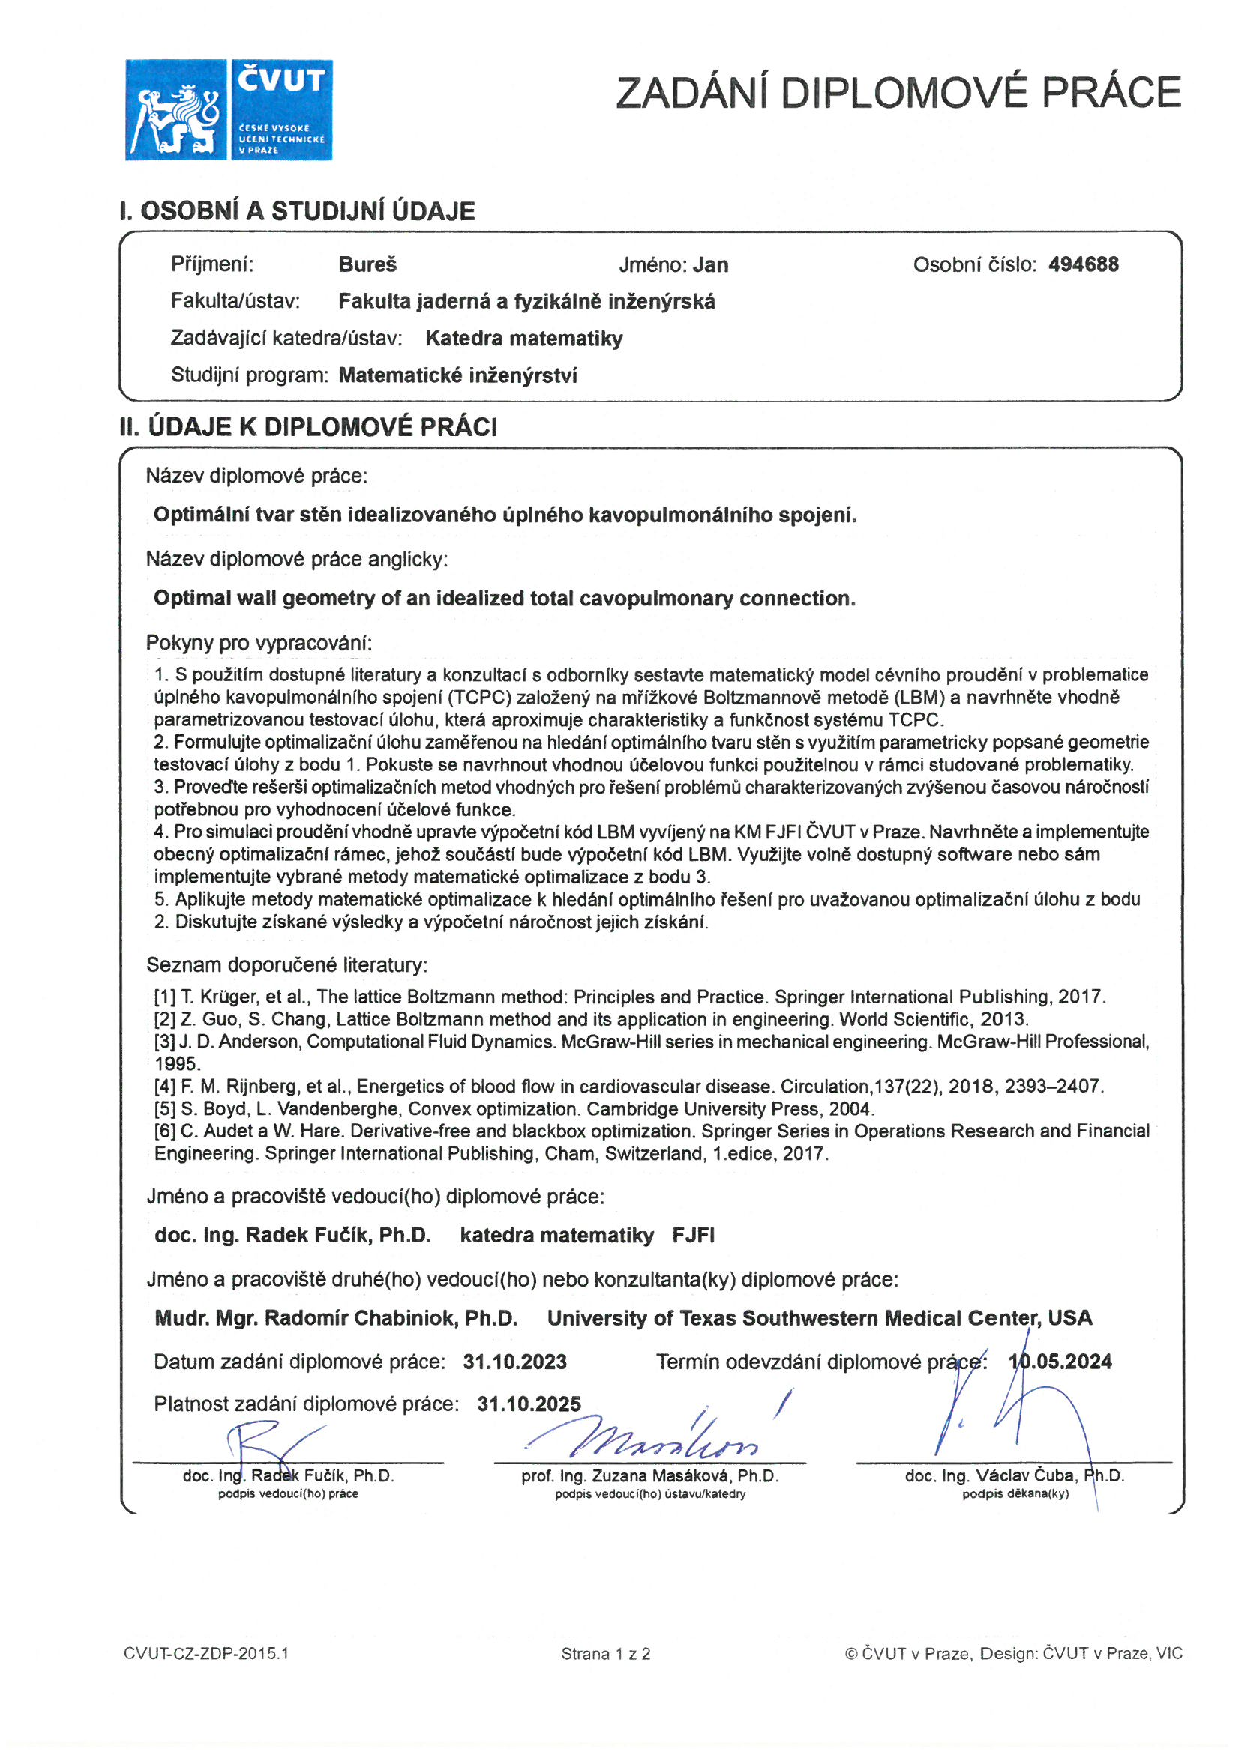
\includepdf[pages=-]{chapters/zadani.pdf}
\noindent \emph{\Large{}Poděkování:}{\Large\par}

\noindent Chtěl bych zde poděkovat především svému školiteli doc. Ing. Radku Fučíkovi, Ph.D.
za nesmírnou pečlivost, ochotu, trpělivost a odborné zázemí při vedení této práce. Dále děkuji svému odbornému konzultantovi Ing. Pavlu Eichlerovi, Ph.D. za rady, cenné poznámky a především za zájem o dané téma. V neposlední řadě mé díky patří MUDr. Mgr. Radomíru Chabiniokovi, Ph.D. za odborné připomínky týkající se medicínské problematiky této práce.

\vfill

\noindent \emph{\Large{}Čestné prohlášení:}{\Large\par}

\noindent Prohlašuji, že jsem tuto práci vypracoval samostatně a uvedl
jsem všechnu použitou literaturu.

\bigskip{}

\noindent V Praze dne 21. května 2023 \hfill{}Jan Bureš

\vspace{2cm}

\newpage{}
%~\newpage{}
\begin{onehalfspace}
\noindent \emph{Název práce:}
\noindent \textbf{Hledání optimálního tvaru stěn matematického modelu proudění krve v problematice úplného kavopulmonálního cévního napojení}
\end{onehalfspace}
\noindent \emph{Autor:} Bc. Jan Bureš\\[2pt]
\noindent \emph{Program:} Matematické inženýrství\\[2pt]
\noindent \emph{Druh práce:} Výzkumný úkol\\[2pt]
\noindent \emph{Vedoucí práce:} doc. Ing. Radek Fučík, Ph.D.,
Katedra matematiky a katedra softwarového inženýrství, FJFI ČVUT v Praze
Trojanova 13, 120 00 Praha\\[2pt]
\noindent \emph{Konzultant:} Ing. Pavel Eichler, Katedra softwarového inženýrství, FJFI ČVUT v Praze
Trojanova 13, 120 00 Praha 2\\[2pt]
\noindent \emph{Abstrakt:} Tato práce se zabývá optimalizací tvaru stěn v rámci modelování proudění nestlačitelné newtonovské tekutiny se zaměřením na modelování proudění krve v cévách. Je představen a implementován optimalizační rámec, který lze následně využít pro řešení optimalizačních úloh týkajících se proudění tekutin okolo rigidních překážek ve 2D. Pro numerické řešení matematického modelu je zvolena mřížková Boltzmannova metoda, která je stručně popsána.
Na hranici obtékaných těles jsou předepsány interpolační okrajové podmínky, které jsou popsány a dále použity. Díky interpolačním okrajovým podmínkám je zohledněn skutečný tvar hranice těles.
V teoretické části jsou pak dále popsány metody matematické optimalizace použité v této práci. Dále je popsán balík využitý k automatickému generování geometrií použitelných v numerických simulací, který byl implementován pro účely této práce. Praktická část demonstruje a analyzuje použití optimalizačního rámce na sérii vhodně navržených testovacích úloh. Na závěr jsou prezentovány výsledky optimalizační úlohy zjednodušeného modelu totálního kavopulmonálního spojení ve 2D, které jsou ve shodě s dostupnou literaturou. Použití optimalizačního rámce lze tedy považovat za úspěšné.

\bigskip{}

\noindent \emph{Klíčová slova:} matematická optimalizace, modelování proudění krve, mřížková Boltzmannova metoda, optimalizace tvarů, úplné kavopulmonární spojení
\vfill{}
~

%Interpolation boundary conditions are prescribed on the boundary of the enveloped bodies, which are described and used below. Due to the interpolation boundary conditions, the actual shape of the boundary of the bodies is taken into account.

\selectlanguage{american}%
\begin{onehalfspace}
\noindent \emph{Title:}
\noindent \textbf{Optimal shape design of walls of blood flow mathematical model focusing on the total cavopulmonary connection}
\end{onehalfspace}
\noindent \emph{Author:} Bc. Jan Bureš\\[2pt]
\noindent \emph{Abstract:} This thesis deals with the optimization of shape of walls and with flow modelling of incompressible Newtonian fluid with a focus on modelling of blood flow in blood vessels. An optimization framework is presented and implemented, which can then be used to solve optimization problems involving fluid flow around rigid objects in 2D. The lattice Boltzmann method is used as the numerical solver and is briefly described. The theoretical section then describes the mathematical optimization methods used in this work. Interpolation boundary conditions, which are described and later used, are prescribed on the boundary of the objects. Thanks to the interpolation boundary conditions, the actual shape of the boundary of the objects is taken into account. Furthermore, the package used to automatically generate geometries used in the numerical simulations, which was implemented for the purpose of this work, is described. The next part demonstrates and analyses the application of the optimization framework on a series of test problems. Finally, the results of the optimization problem of a simplified 2D total cavopulmonary connection model are presented, which are in agreement with the available literature. Thus, the application of the optimization framework can be considered successful.

\bigskip{}

\noindent \emph{Key words:} mathematical optimization, modeling of blood flow, lattice Boltzmann method, shape optimization, total cavopulmonary connection
\selectlanguage{czech}%
\newpage{}

%~\newpage{}

\pagestyle{plain}

\tableofcontents{}

\newpage{}

\chapter*{Úvod}

\addcontentsline{toc}{chapter}{Úvod}

Tato práce se zabývá matematickým modelováním proudění tekutin se zaměřením na hledání optimálního tvaru stěn zejména v problematice úplného kavopulmonálního cévního napojení. V mnoha inženýrských odvětvích jako je např. automobilový nebo letecký průmysl je zapojení procesu optimalizace pro nalezení optimálního tvaru zkoumaného objektu běžnou praxí. V oblasti klinické medicíny však obecně z řady důvodů využití optimalizačních technik stále není tak obvyklé. Pro získání relevantních výsledků je totiž potřeba co nejpřesněji modelovat komplexní proudění krve uvnitř mnohdy složitých geometrií za použití důkladně otestovaných metod. Validace výsledků numerických simulací vůči naměřeným datům je pak také často složitá, jelikož provádění experimentů \textit{in vivo} (v živém organismu) je z~přirozených důvodů velmi obtížné, někdy až nemožné.

Přesto však proces optimalizace tvarů může zejména v kardiochirurgii a cévní chirurgii nacházet velký potenciál \cite{Abraham2005, Weddell2015, Marsden2008}. Vyvinutí optimalizačního procesu použitelného v medicínském prostředí by pro lékaře představovalo \textit{in vitro} (mimo živý organismus) způsob, jak posuzovat chirurgický zákrok v rámci geometrie specifické pro daného pacienta. Navrhování a implantování objektů jako je stent či umělá chlopeň by pak bylo přizpůsobené přímo anatomii pacienta, což může vést ke zlepšeným klinických výsledků, ke snížení rizika pooperačních komplikací a k obecnému zlepšení kvality života pacienta po zákroku \cite{Marsden2008}.

Příkladem konkrétního chirurgického zákroku, kde může proces optimalizace tvaru stěn najít své uplatnění, je tzv. úplné kavopulmonální spojení (anglicky \textit{total cavopulmonary connection}, dále jen TCPC). TCPC se provádí u~dětí, u nichž je diagnostikována tzv. funkčně jediná komora, tj. u~pacientů se závažnou vrozenou srdeční vadou, kvůli které je jejich srdce schopno efektivně využít pouze jednu funkční komoru, a~u~nichž nelze chirurgicky zajistit fungující dvoukomorovou cirkulaci \cite{Chaloup}. Jedná se o~operaci, při které je horní dutá žíla (\textit{vena cava superior}, ozn. \textit{d} na obr. \ref{fig:tcpc}) chirurgicky napojena na plicnici. Také dolní dutá žíla (\textit{vena cava inferior}, ozn. \textit{b} na obr. \ref{fig:tcpc}) je napojena přímo na plicnici (\textit{arteria pulmonalis}, ozn. \textit{a} na obr. \ref{fig:tcpc}) a~to zpravidla pomocí tzv. extrakardiálního konduitu (ozn. \textit{c} na obr. \ref{fig:tcpc}), neboli mimosrdečního kanálu, vytvořeného z cévní protézy \cite{Rubtsova, Delorme}. 

\begin{figure}[h]
	\centering
	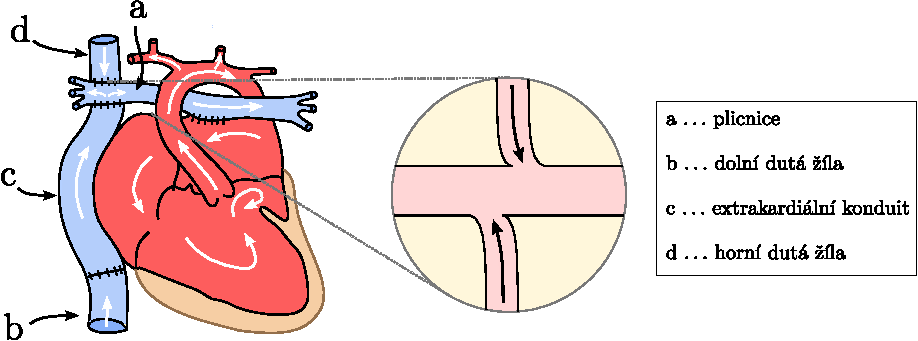
\includegraphics[width=0.84\textwidth]{Images/srdce-zoom.pdf}
	\caption{Schéma úplného kavopulmonálního spojení. Zvětšená část zobrazuje místo napojení mimosrdečního kanálu.}
	\label{fig:tcpc}
	\vspace{-2mm}
\end{figure}

TCPC umožňuje vytvořit funkční oběh krve, vzniklý systém cirkulace je však specifický a je citlivý na vícero faktorů, které nežádoucím způsobem přispívají ke ztrátě energie v systému. To postupně vede k~celkovému selhání systému. Jedná se zejména o vlivy turbulentního proudění a kolize proudů, ke kterým dochází například ve vyústění horní a dolní duté žíly do plicnice. Právě problematika optimálního napojení extrakardiálního konduitu za účelem minimalizace ztráty energie či minimalizace namáhání tkáně může být předmětem procesu optimalizace \cite{Chaloup, vanBake, Wang}. Existuje řada studií zabývající se návrhem optimálního tvaru napojení konduitu, často se však opírají pouze o metodu "pokus-omyl" a~metody optimalizace nepoužívají \cite{Rijnberg2018, Porfiryev2020, Tang2014}.

Pro vytvoření optimalizačního rámce použitelného pro kardiochirurgii při simulování proudění krve je nutné použít k výpočtu hodnot účelové funkce, jež je předmětem minimalizace, efektivní a spolehlivou numerickou metodu. V rámci této práce využijeme k numerickým výpočtům mřížkovou Boltzmannovu metodu (anglicky \textit{lattice Boltzmann method}, dále jen LBM). Poznamenejme, že pro metodu LBM byl použit kód, který je vyvíjený na katedře matematiky FJFI ČVUT v Praze a který byl dle potřeb této práce upraven. Hlavní výhodou LBM je možnost masivní paralelizace na GPU (grafických procesorech), díky čemuž výpočty trvají řádově kratší dobu, než u standardních numerických metod využívaných k~modelování proudění tekutin \cite{PE, Kruger}. Naopak podstatnou nevýhodou LBM z hlediska geometrie hranic je, že pro prostorovou diskretizaci využívá pravidelnou mřížku. To představuje v kontextu této práce výrazný problém, jelikož hranice obtékáných těles nebo hranice cév jsou diskretizovány schodovitě. Proto je část této práce i předchozí bakalářské práce \cite{JB} věnována studiu a implementaci interpolačních okrajových podmínek, které umožňují v rámci diskretizace obtékaných těles zohlednit skutečný tvar jejich hranice. Díky použití těchto okrajových podmínek pak i malá změna tvaru geometrie použité v rámci numerické simulace vede ke změně výsledku získaného pomocí numerické simulace, proto lze v rámci optimalizace využít i např. gradientní optimalizační metody.

Struktura práce je následující. První kapitola se zaměřuje na matematický model proudění tekutin s důrazem na model proudění krve v cévách. Druhá kapitola podrobně rozebírá použitou numerickou metodu LBM. V třetí kapitole je dále rozebrán nástroj vyvinutý pro efektivní parametrizaci a následné automatické generování geometrie. Čtvrtá kapitola obsahuje teorii matematické optimalizace a optimalizační metody použité v této práci, dále je v této kapitole představen navržený použitý optimalizační rámec. Poslední kapitola představuje výsledky provedených numerických simulací. Nejdříve je otestována funkčnost použitého optimalizačního rámce na sérii navržených testovacích úloh s jedním optimalizačním parametrem. Dále je optimalizace testována na složitějších úlohách s více optimalizačními parametry a je mimo jiné zkoumán vliv použité optimalizační metody a volby počátečního odhadu řešení. Jedna ze složitějších úloh zahrnuje zjednodušený 2D model cévní křižovatky vznikající při úplném kavopulmonálním napojení.



\chapter{Matematický model proudění krve}\label{mmodel}
V této kapitole popíšeme základní vztahy týkající se dynamiky kontinua relevantní pro tuto práci. Představíme rovnice popisující proudění ve volném prostředí. Popíšeme turbulentní chování a Reynoldsův rozklad. Dále uvedeme některé z charakteristik důležité pro popis proudění krve v cévách. Na závěr shrneme předpoklady, které jsou dále kladeny na matematický model použitý v této práci.

\section{Dynamika tekutin}
Budeme považovat zkoumanou tekutinu za kontinuum, tedy ji budeme považovat za dokonale spojitou strukturu. Rovnice popisující dynamiku kontinua lze jednoznačně odvodit ze zákonů záchování hmoty, hybnosti a energie. Dále jsou tyto rovnice spjaty s fyzikálními vlastnostmi zkoumaného prostředí a materiálu. 

V izolovaném a izotermálním systému lze vývoj dynamiky tekutiny v čase vyjádřit pomocí soustavy parciálních diferenciálních rovnic ve tvaru
\\
\begin{subequations}\label{NS}
	\begin{gather}
	\label{a}
	\frac{\partial \rho}{\partial t} + \nabla \cdot (\rho \vec{u}) = 0, \\[5pt]
	\label{b}
	\frac{\partial (\rho \vec{u})}{\partial t} + \nabla \cdot (\rho \vec{u} \otimes \vec{u}) = \nabla \cdot \mathbf{T} + \rho \vec{g},
	\end{gather}
\end{subequations}
kde symbol $ \otimes $ značí vnější součin definovaný po složkách jako $ (\vec{u} \otimes \vec{u})_{ij} = u_{i} u_{j}, \: i,j \in \{1,2,3\} $ \cite{Anderson}. Veličiny v \eqref{NS} značí postupně
\begin{itemize}
	\item[]{\makebox[3cm]{$ \rho $ \si{[kg.m^{-3}]}\hfill} hustotu tekutiny,}
	\item[]{\makebox[3cm]{$ \vec{u} $ \si{[m.s^{-1}]}\hfill} vektor makroskopické rychlosti,}
	\item[]{\makebox[3cm]{$ \mathbf{T} $ \si{[kg.m^{-1}.s^{-2}]}\hfill} úplný tenzor napětí,}
	\item[]{\makebox[3cm]{$ \vec{g} $ \si{[m.s^{-2}]}\hfill} vektor zrychlení vnějších sil.}
\end{itemize}
Všechny veličiny v \eqref{NS} jsou obecně funkcemi času $ t $ \si{[s]} a polohy $ \vec{x} $~\si{[m]}.

Izotermální systém lze doplnit o stavovou rovnici ideálního plynu ve tvaru
\begin{equation}\label{pressure}
p = c^{2}_{s} \ \rho,
\end{equation}
kde $ p $ \si{[Pa]} značí tlak a $ c_{s} $ \si{[m.s^{-1}]} je rychlost zvuku v dané tekutině \cite{Latt}. V tomto případě \eqref{NS} společně s \eqref{pressure} tvoří uzavřený systém, který lze řešit bez použití zákona zachování energie.

\subsection{Tenzor napětí a silové působení}

Dynamický tenzor napětí budeme značit $\mathbf{T}_{\mu} = \big(\sigma^{\, \mu}_{ij} \,\big)$ \si{[kg.m^{-1}.s^{-2}]}, kde $ i,j \in \{1,2,3\} $. Pro newtonovské tekutiny platí, že složky dynamického tenzoru napětí jsou lineárně závislé na prostorových derivacích rychlosti. Tekutiny, které tuto lineární závislost nesplňují, se nazývají nenewtonovské. Pro složky dynamického tenzoru napětí newtonovských tekutin platí, že \cite{Schlichting}

\begin{subequations}\label{newton}
	\begin{eqnarray}
	\sigma^{\, \mu}_{ii} = \lambda \nabla \cdot \vec{u} + 2 \mu \frac{\partial u_i}{\partial x_i},&& \hspace{-3mm} i \in \{1,2,3\}, \\[5pt]
	\sigma^{\, \mu}_{ij} = \sigma^{\, \mu}_{ji} = \mu \ \left( \frac{\partial u_i}{\partial x_j} + \frac{\partial u_j}{\partial x_i} \right),&& \hspace{-4mm} \ i,j \in \{1,2,3\}, \: i \neq j,
	\end{eqnarray}
\end{subequations}
kde $ \mu $ \si{[kg.m^{-1}.s^{-1}]} označuje dynamickou viskozitu a $ \lambda $ \si{[kg.m^{-1}.s^{-1}]} je tzv. druhý viskózní koeficient~\cite{Cengel}. Pro newtonovské tekutiny je $ \mathbf{T}_{\mu} $ zjevně symetrický tenzor. Zavedeme-li dále tenzor rychlosti deformace~$ \mathbf{D}~$ \si{[s^{-1}]} vztahem

\begin{equation}\label{eq:D}
\mathbf{D} = \frac{1}{2} \left[ \nabla \vec{u} \ + \ (\nabla \vec{u})^T \right],
\end{equation}
lze dynamický tenzor napětí ekvivalentně přepsat do tvaru

\begin{equation}\label{eq:1}
\mathbf{T}_{\mu} = 2 \mu \mathbf{D} \ + \ \left( \lambda + \frac{2}{3} \mu \right) \ (\nabla \cdot \vec{u}) \  \mathbf{I} \ ,
 \end{equation}
kde $ \mathbf{I} $ je jednotkový tenzor odpovídajícího rozměru. S použitím Stokesovy hypotézy, $ \lambda = -\frac{2}{3} \mu $ \cite{Anderson}, dávající do souvislosti dynamickou viskozitu a druhý viskózní koeficient, přejde vztah \eqref{eq:1} do tvaru

\begin{equation}
\mathbf{T}_{\mu} = 2 \mu \mathbf{D}.
\end{equation}
Pomocí $\mathbf{T}_{\mu}$ můžeme dále úplný tenzor napětí pro newtonovskou tekutinu psát ve tvaru
\begin{equation}\label{eq:T}
\mathbf{T} = -p\mathbf{I} + \mathbf{T}_{\mu},
\end{equation}
kde $ \mathbf{I} $ je opět jednotkový tenzor odpovídajícího rozměru \cite{Cengel}.

Tenzor rychlosti deformace se dále používá pro definici smykové rychlosti $ \dot{\gamma} $~\si{[s^{-1}]} (anglicky \textit{shear rate}) \cite{Cengel} vztahem
\begin{equation}\label{eq:dot gamma}
\dot{\gamma}  = \sqrt{2} \| \mathbf{D} \| _{F},
\end{equation}
kde $ \| \cdot \| _{F} $ značí Frobeniovu maticovou normu definovanou pro obecnou matici $ \mathbf{A} $ s rozměry $ m \times n $ s prvky $ a_{ij} $ jako
\begin{equation}
\| \mathbf{A} \| _{F}  \coloneqq \sqrt{\sum_{i = 1}^{m} \sum_{j = 1}^{n} |a_{ij}|^2}.
\end{equation}

Je-li předmětem zkoumání silové působení tekutiny na hranici objektu $ \partial \Omega $, můžeme s využitím \eqref{eq:T} vyjádřit složky celkové síly působící na $ \partial \Omega $ jako

\begin{equation}\label{eq:stress_int}
{F}_{i} = \int\limits_{\partial\Omega}(\mathbf{T} \vec{n})_{i} \mathrm{d}S, \hspace{2mm} i \in \{1,2,3\},
\end{equation}
kde $ \vec{n} $ značí normálový vektor hranice $ \partial \Omega $. Takto vyjádřená síla představuje součet působení tlakových a~viskózních sil.

Pro popis interakce tekutiny s překážkou se dále často používá smykové napětí působící na stěně (anglicky \textit{wall shear stress}) \cite{WallStress}, které budeme značit $ \tau _w $ \si{[kg.m^{-1}.s^{-2}]} a které je ve 2D definované vztahem
\begin{equation}\label{eq:wall shear stress}
\tau_w = \mathbf{T} \cdot \vec{t},
\end{equation}
kde $ \vec{t} $ značí jednotkový vektor tečný na stěnu v daném bodě.

\subsection{Turbulence a Reynoldsův rozklad}\label{turb}
Turbulentním budeme nazývat takové proudění, které je v čase i prostoru neuspořádané. Směr a velikost rychlosti turbulentního proudění se neustále mění, dochází k obecně nepravidelným fluktuacím. Turbulentní proudění vykazuje náhodný a nestabilní charakter.

Turbulentní proudění je možné pozorovat při vyšších hodnotách Reynoldsova čísla, což je bezrozměrná veličina definovaná jako
\begin{equation}\label{Re}
\mathrm{Re} = \dfrac{l_{0} u_{0}}{\nu} = \dfrac{l^{2}_{0}}{t_{0} \nu},
\end{equation}
kde $ \nu $ je kinematická viskozita \si{[m^2.s^{-1}]}, dále $ l_{0} $~\si{[m]}, $ t_{0} $ \si{[s]} a $ u_{0} $~\si{[m.s^{-1}]} jsou po řadě charakteristická délka, charakteristický čas a charakteristická rychlost specifické pro zkoumanou úlohu \cite{Landau}.

Z popsaných vlastností turbulentního proudění je patrné, že jeho popis je obtížný. Jedním z přístupů, jak turbulentní proudové pole popsat, je pomocí statistického přístupu, Reynoldsova časového průměrování veličin \cite{Sodja2007}, při kterém dochází k dekompozici dané veličiny $ \psi $ na její střední hodnoty $ \overline{\psi} $ a fluktuace $ \psi ' $ jako
\begin{equation}
	\psi = \overline{\psi} + \psi '.
\end{equation}
Fluktuace $ \psi ' $ jsou definovány tak, že střední hodnota $ \overline{\psi '} $ přes jeden časový úsek musí být nulová \cite{Schlichting}.

%Střední hodnotu můžeme získat
%\begin{itemize}
%	\item středováním v čase, tj.
%	$$ \overline{\psi} _T (\vec{x}) = \lim_{T \to +\infty} \frac{1}{T} \int\displaylimits_{t}^{t+T} \psi(\vec{x}, \tau) \, \text{d} \tau, $$
%	\item středováním v prostoru,
%	$$ \Big[ {\psi} _V (t) \Big]= \lim_{|V( \vec{x})| \to +\infty} \frac{1}{|V( \vec{x})|} \int\displaylimits_{|V( \vec{x})|}^{} \psi(\vec{\xi}, t) \, \text{d} \vec{\xi}, $$
%	kde $ \vec{x} \in V(\vec{x})$,
%	\item středováním přes statistický soubor ($ N $ opakováním identického procesu),
%	$$ \Big\{ {\psi} _N (\vec{x}, t) \Big\} = \lim_{N \to +\infty} \frac{1}{N} \sum_{k \in N}^{} \psi(\vec{x}, t) .$$
%\end{itemize}
Zdůrazněme, že $ \psi $ v tomto případě představuje libovolnou skalární veličinu, za kterou můžeme volit např. složky rychlosti $ \vec{u}_i $, tlak $ p $ či hustotu $ \rho $ \cite{Sodja2007}. Dále podotkněme, že v praxi je důležité, aby časový interval pro průměrování
%, resp. kontrolní objem,
měl řádově větší velikost než je tomu u časového
%, resp. prostorového měřítka
turbulentních jevů, které chceme popisovat \cite{Sodja2007}.

Omezíme-li se nyní na Reynoldsův rozklad rychlostního pole $ \vec{u} (\vec{x}, t) $ ve smyslu průměrování v čase, můžeme zavést turbulentní kinetickou energii $ T_{\text{turb}} $~\si{[m^{2}.s^{-2}]} vztahem
\begin{equation}\label{eq:turb kin energy}
	T_{\text{turb}} = \dfrac{1}{2} \left( \overline{(u_1 ')^2} + \overline{(u_2 ')^2} + \overline{(u_3 ')^2} \right) = \dfrac{1}{2} \left( \overline{(u_1 ')^2 + (u_2 ')^2 + (u_3 ')^2} \right),
\end{equation}
kde jsme použili pravidla pro aritmetiku při používání Reynoldsova rozkladu \cite{Sodja2007}.

\section{Popis cévního proudění}\label{cevni proudeni}
Z důvodu přítomnosti řady fyzikálních, chemických a fyziologických procesů představuje cévní proudění velmi komplexní proces. V mnoha případech však postačí k jeho popisu zjednodušený model zanedbávající některé z charakteristik \cite{Saloner2019}. V této sekci krátce popíšeme některé z aspektů, u nichž lze za vhodných předpokladů uvážit zjednodušený model.

\section*{\fontsize{11}{15}\selectfont Elasticita stěn}
Interakce elastického tělesa, tedy tělesa s pohyblivou hranicí, lze při modelování realizovat např. použitím metody vnořené hranice (anglicky \textit{immersed boundary method}) \cite{Peskin}. V mnoha případech však můžeme elasticitu stěn překážky zanedbat a uvažovat pouze rigidní geometrii. Zejména v oblasti menších cév se ukazuje, že zanedbání elasticity cévních stěn nemá významný efekt na výsledek. \cite{DempereMarco2006} To však neplatí vždy, jelikož např. v oblasti aorty byly při uvažování rigidní geometrie pozorovány výraznější nezanedbatelné vlivy na celkovou chybu výsledku. \cite{LANTZ2011}

Poznamenejme, že pro zahrnutí elasticity cévních stěn do uvažovaného modelu je potřebné vhodně stanovit podmínky interakce s tekutinou, což je v rámci cévního proudění obecně obtížný úkol mnohdy závisející na správném vyhodnocení \textit{in vivo} měření. Kromě toho při onemocněních jako je arterioskleróza\footnote{Arterioskleróza je onemocnění, při němž dochází ke zvětšení tloušťky stěn tepen a k jejich následné ztrátě elasticity \cite{Fishbein2015}.} ztrácí cévy u řady pacientů svou pružnost, tedy zahrnutí elasticity do modelu nutně nemusí korektně reflektovat fyziologický stav cév \cite{Saloner2019}.

\section*{\fontsize{11}{15}\selectfont Viskozita krve}

Pro matematický model je důležité správně volit hodnoty viskozity tak, aby v sobě zahrnovaly případné nenewtonovské chování zkoumané tekutiny. Většinou se krev považuje za newtonovskou tekutinu. Nicméně existují situace, kdy je newtonovské chování krve porušeno. Na jednu stranu v případech, kdy je rychlost proudění krve velmi malá, se červené krvinky mohou hromadit a v důsledku toho viskozita krve vzrůstá.
Oblasti s takto pomalým prouděním lze najít např. v oblastech aneurysmatické dilatace\footnote{Aneurysmatickou dilatací se rozumí onemocnění, při kterém dochází k lokálnímu rozšíření cévy \cite{Syed1997}.}. Na druhou stranu viskozita krve výrazně klesá v oblastech, kde krev teče skrz velmi úzké cévy, to zejména skrze cévy na úrovni měřítka arteriol či kapilár \cite{Saloner2019}.
	
Existují modely viskozity, které se snaží přesněji zachytit fyzikální popis a chování viskozity krve~\cite{Saloner2019, Eichler2023, Boyd2007}. Nejjednodušší je tzv. mocninný model (anglicky \textit{Power-Law model}) \cite{Sequeira}. Mocninný model předepisuje pro viskozitu 
\begin{equation}\label{eq:power-law}
\mu _{\text{PL}} (\dot{\gamma}) = K_p  \dot{\gamma} ^{n_1-1} \ ,
\end{equation}
kde $ K_p$ \si{[kg.m^{-1}]} a $ n_1 $ \si{[-]} jsou konstanty. Dalším modelem je Cassonův model  \cite{Boyd2007} splňující
\begin{equation}\label{eq:Casson}
	\mu _{\text{CA}} (\dot{\gamma}) = \frac{1}{\dot{\gamma}} \left[ k_{0} + k_{1} \sqrt{\dot{\gamma}} \right]^2 \ ,
\end{equation}
kde $ k_1$ \si{[kg^{2}.m^{-2}]} a $  k_2 $ \si{[kg^{2}.m^{-2}]} jsou konstantní parametry určené empiricky. Hlavní výhodou těchto základních modelů je to, že v určitých geometriích a za konkrétních daných podmínek jsou pro ně k dispozici exaktní řešení, což např. poskytuje referenční hodnoty pro numerické simulace. Zjevnou nevýhodou těchto modelů je jejich omezená použitelnost, jelikož pro hodnoty smykové rychlosti blížící se nule selhávají \cite{Boyd2007}.

Mezi komplexnější modely lze řadit Crossův model \cite{Sequeira} definovaný vztahem
\begin{equation}\label{eq:cross}
\mu _{\text{CR}} (\dot{\gamma}) = \frac{\mu_{0} - \mu_{\infty}}{1 + (k\dot{\gamma})^{n_2}} + \mu_{\infty}  \ ,
\end{equation}
kde $ k $ \si{[s]} a $ n_2 $ \si{[-]} jsou konstanty a dále platí
\begin{equation}\label{eq:m0 a minf}
\mu _{0}  = \lim_{\dot{\gamma} \rightarrow 0+}\mu (\dot{\gamma})\, , \ \mu_{\infty} = \lim_{\dot{\gamma} \rightarrow \infty}\mu (\dot{\gamma}).
\end{equation}
Posledním zmíněným modelem je Carreaův-Yassudův model \cite{Boyd2007} splňující
\begin{equation}\label{eq:C-Y}
\mu _{\text{CY}} (\dot{\gamma}) = \mu_{\infty} + (\mu_{0} - \mu_{\infty}) \left[ 1 + (\varepsilon \dot{\gamma}) ^{a} \right]^{\frac{n_3-1}{a}} \ ,
\end{equation}
kde $ \varepsilon$ \si{[s]} , $a$ \si{[-]} a $ n_3 $ \si{[-]} jsou opět empiricky určené konstantní parametry, které ovlivňují chování modelu mezi hraničními hodnotami viskozity. Pro $ \mu_{0}$ a $ \mu_{\infty} $ opět platí \eqref{eq:m0 a minf}.


Srovnání všech zmíněných modelů je k nahlédnutí na obr. \ref{fig:vs}, hodnoty parametrů byly převzaty z~\cite{Eichler2023}.

\begin{figure}[H]
	\centering
	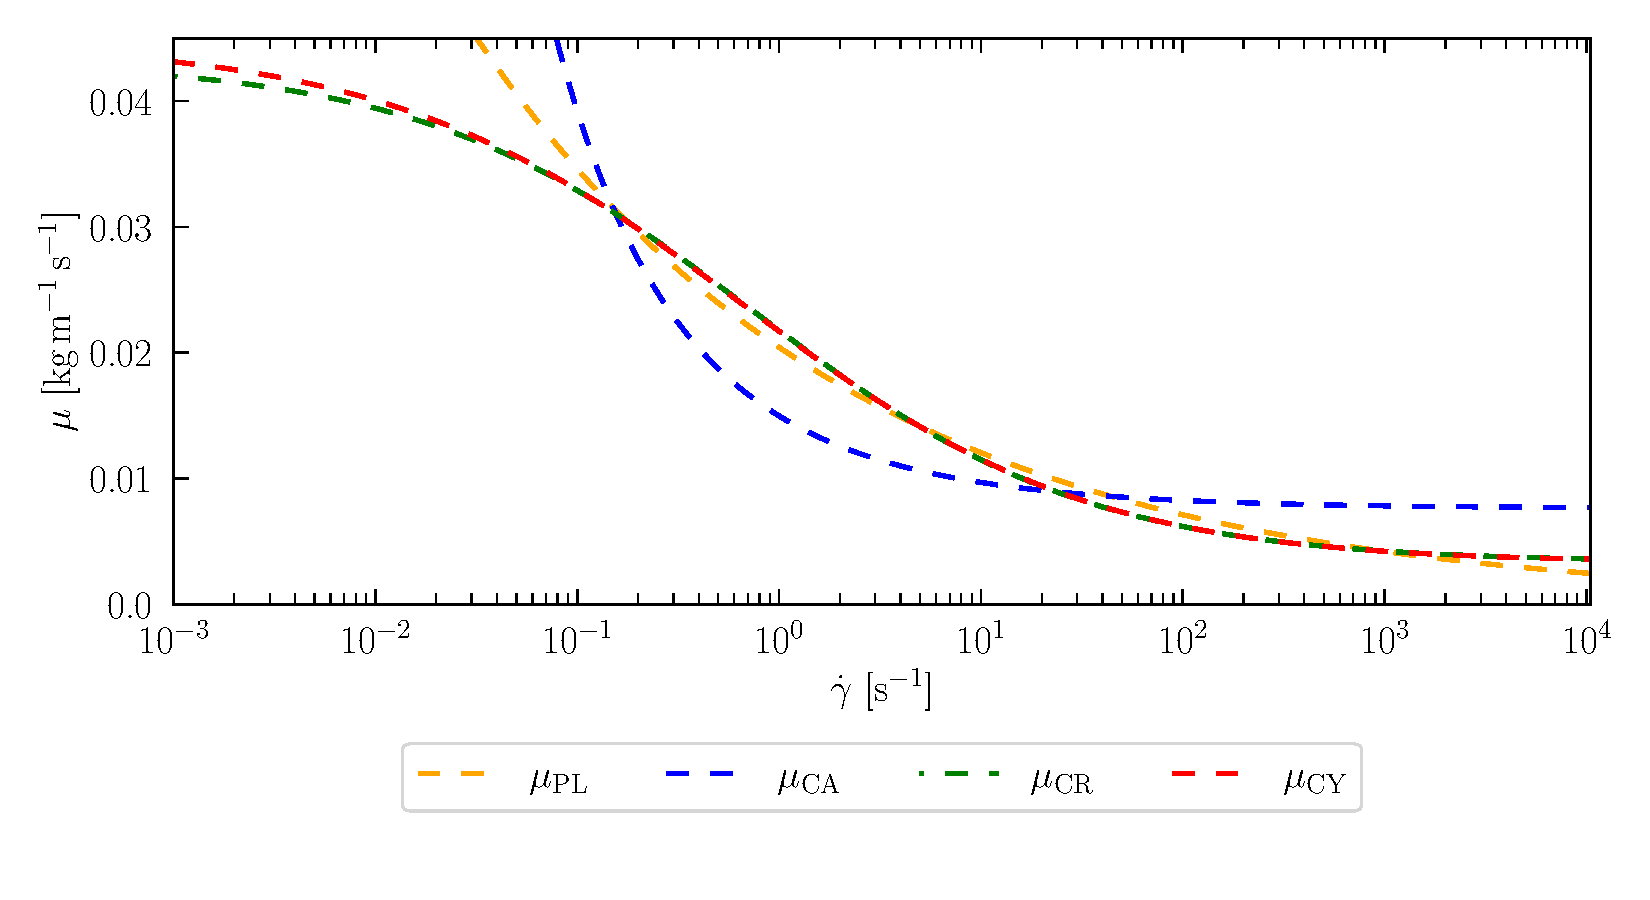
\includegraphics[width=1.0\textwidth]{Images/modely.pdf}
	\vspace{-9mm}
	\caption{Srovnání nenewtonovských modelů viskozity, konkrétní hodnoty parametrů byly převzaty z \cite{Eichler2023}. Popisy jednotlivých modelů odpovídají definujícím vztahům
    \eqref{eq:power-law}, \eqref{eq:Casson}, \eqref{eq:cross} a \eqref{eq:C-Y}}.
	\label{fig:vs}
\end{figure}

Podotkněme, že v rámci této práce budeme dále uvažovat krev výhradně jako newtonovskou tekutinu.

\section*{\fontsize{11}{15}\selectfont Turbulentní proudění}
Proudění krve je ve většině případů aproximovatelné pomocí laminárního proudění \cite{Sequeira}. V některých případech však v cévním proudění dochází k výskytu turbulencí a chaotického chování \cite{Saqr2020}. Jedna z~oblastí, kde lze turbulence pozorovat, je oblast nacházející se za cévní stenózou\footnote{Stenóza cévy je onemocnění, při němž dochází k jejímu lokálnímu zúžení  \cite{Carabello2009}.} \cite{Jain2022}. Rychlost proudění krve ve zúžené oblasti může výrazně vzrůstat, zmenšení průměru cévy však zajistí, že proudění setrvá v této části zúžení laminární \cite{Sequeira}. Avšak bezprostředně za zúžením rychlost proudění zůstavá zvýšená i~v~oblasti s původním průměrem, což může vést ke vzniku vírů a změně režimu proudění \cite{Saloner2019, Varghese2003}.

Výskyt turbulentního proudění je z fyziologického hlediska nežádoucí, jelikož je často doprovázen značnou disipací kinetické energie, kvůli níž můžou být části oběhové soustavy více namáhány. Mimoto cévní oblasti s výskytem turbulencí vykazují zvýšenou námahu na stěny cév, což může vyústit až k~narušení tkáně a k nemocem jako je např. arterioskleróza. Je tedy žádoucí turbulence v proudění krve minimalizovat \cite{Saloner2019, Kameneva2004}. 

\section{Předpoklady matematického modelu v této práci}\label{pred}
Na závěr shrneme, jaké dodatečné předpoklady budeme uvažovat v našem systému. Díky těmto předpokladům se řešení systému \eqref{NS} zjednoduší. Konkrétně budeme v rámci této práce uvažovat pouze izotermální systém (tj. jeho teplota je v čase konstantní), na který nepůsobí žádné vnější síly. Uvažovaná tekutina je dále nestlačitelná, newtonovská a s konstantní dynamickou viskozitou.

Budeme uvažovat obdélníkovou oblast $ \Omega \subset \mathbb{R}^2 $, $ \Omega = (0, L_1) \times (0, L_2) $, kde $ L_1, L_2 $ \si{[m]} jsou velikosti stran obdélníka, a časový interval $ \mathcal{I} = \langle 0, T \rangle,$ kde $ T > 0$. Označíme 

Rovnice \eqref{NS} řešené na $ \Omega \times \mathcal{I} $ se s uvažovanými předpoklady redukují na \cite{Schlichting}

\begin{subequations}\label{NS s predpoklady}
	\begin{gather}
	\label{a s predpoklady}
    \nabla \cdot \vec{u} = 0, \\[5pt]
	\label{b s predpoklady}
	\rho \frac{\text{D} \vec{u}}{\text{D} t} = - \nabla p + \mu \Delta \vec{u},
	\end{gather}
\end{subequations}
kde jsme využili zápisu pomocí operátoru materiálové derivace 
\begin{equation}
	\dfrac{\text{D}}{\text{D} t} \coloneqq \dfrac{\partial}{\partial t} + \vec{u} \cdot \nabla.
\end{equation}

Označíme $ \partial \Omega_{\text{in}} $ část hranice oblasti $ \Omega $, kde předepisujeme okrajovou podmínku na vstupu, dále $ \partial \Omega_{\text{out}} $ část hranice oblasti $ \Omega $, kde předepisujeme okrajovou podmínku na výstupu, a $ \partial \Omega_{\text{w}} $ část hranice, kde se nachází rozhraní mezi tekutinou a tělesem a kde uvažujeme no-slip okrajovou podmínku. Poté rovnice jsou rovnice \eqref{NS s predpoklady} doplněny počátečními a okrajovými podmínkami
\begin{subequations}\label{eq:okrajovky}
	\begin{alignat}{3}
	&\vec{u} = \vec{u}_{\text{ini}},  &p = p_{\text{ini}} \hspace{5mm} &\text{na } \ \Omega \times \mathcal{I}\\[3pt]
    &(\nabla p - \nu \Delta \vec{u}) \cdot \vec{n}  = 0, &\vec{u} = \vec{u}_{\text{in}} \hspace{5mm} &\text{na } \ \partial \Omega_{\text{in}} \times \mathcal{I}\\[3pt]
	&\vec{u} = \vec{0}, \, &\nabla p \cdot \vec{n} = 0 \hspace{5mm} &\text{na } \ \partial \Omega_{\text{w}} \times \mathcal{I}\\[3pt]
    &p = p_{\text{out}}, &\nabla u_i \cdot \vec{n} = 0 \hspace{5mm} &\text{na } \ \partial \Omega_{\text{out}} \times \mathcal{I}, \, i = 1, 2 \ ,
	\end{alignat}
\end{subequations}
kde $ \vec{n} $ je jednotkový vnější normálový vektor hranice uvažované oblasti, $ \vec{u}_{\text{ini}}$ \si{[m.s^{-1}]} resp. $ p_{\text{ini}} $ \si{[kg.m^{-1}.s^{-2}]} je počáteční rychlost, resp. počáteční tlak, dále $ \vec{u}_{\text{in}}$ \si{[m.s^{-1}]} je rychlost předepsaná na vstupu a $ p_{\text{out}} $~\si{[kg.m^{-1}.s^{-2}]} je tlak předepsaný na výstupu. Počáteční a okrajové podmínky jsou dále diskutovány v sekci~\ref{pocatecni a okrajove podminky}.
\chapter{Mřížková Boltzmannova metoda}\label{lbm}
Tekutinu můžeme považovat za kontinuum a využít makroskopického popisu, tedy nahlížet na tekutinu jako na celek a využívat ke stavovému popisu makroskopické veličiny jako je hustota, rychlost proudění nebo tlak, řídícími je rovnicemi je pak \eqref{NS}. Dále naopak můžeme popisovat dynamiku každé z částic v daném objemu a využít tak mikroskopického popisu. Popsat dynamiku částice na mikroskopickém měřítku není obtížné, avšak značným nedostatkem tohoto přístupu je jeho zjevná výpočetní náročnost, která je přímo úměrná počtu zkoumaných částic.

Mezistupněm mezi výše zmíněnými popisy je popis mezoskopický \cite{PE}, který je založen na kinetické teorii. Tekutina je popsána pomocí jednočásticových pravděpododobnostních distribučních funkcí hustoty $ f(\vec{x},\vec{\xi}, t) $ \si{[kg.s^3.m^{-6}]}, popisujících systém v prostoru souřadnic $ \vec{x} $, mikroskopických rychlostí $ \vec{\xi} $ a čase $ t $. Distribuční funkce $ f $ udávají hustotu částic vyskytujících se v okolí~$ \vec{x} $, v čase~$ t $ mající mikroskopickou rychlost~$\vec{\xi}$.

Jednočásticové distribuční funkce v okolí $ \vec{x} $ splňují Boltzmannovu transportní rovnici \cite{Kruger}
\begin{equation}\label{eq:BTR}
\frac{\partial f}{\partial t} + \sum_{i = 1}^{3} \xi _{i} \frac{\partial f}{\partial x_{i}} + \sum_{i = 1}^{3} g_{i} \frac{\partial f}{\partial \xi _{i}} = \mathcal{C}(f), 
\end{equation}
kde $ \vec{g} $ \si{[m.s^{-2}]} je vektor zrychlení působení vnějších sil a $ \mathcal{C}(f)$ \si{[kg.s^2.m^{-6}]} je kolizní operátor, který bude více rozebrán později v sekci \ref{kol}.

Pomocí distribučních funkcí $ f $ lze vyjádřit některé makroskopické veličiny jako statistické momenty \cite{Kruger}, platí např.

\begin{subequations}\label{eq:macroscopic basic}
	\begin{alignat}{1}
		\rho(\vec{x}, t) & =\int\displaylimits_{\mathbb{R}^3} f(\vec{x}, \vec{\xi}, t) \mathrm{~d} \vec{\xi} \label{subeq:rho}, \\
		\rho(\vec{x}, t) \vec{u}(\vec{x}, t) & =\int\displaylimits_{\mathbb{R}^3} f(\vec{x}, \vec{\xi}, t) \, \vec{\xi} \mathrm{~d} \vec{\xi} \label{subeq:momentum}.
	\end{alignat}
\end{subequations}

Mřížková Boltzmannova metoda (LBM) je numerická metoda vyvinutá na konci dvacátého století, která je založená na mezoskopickém popisu tekutiny. Numerické schéma LBM lze odvodit diskretizací~\eqref{eq:BTR}. V rámci LBM je diskretizace prostoru realizována diskrétní ekvidistantní mřížkou (anglicky \textit{lattice}) a diskretizace prostoru rychlostí pomocí konečné množiny mikroskopických rychlostí. Zavádíme rychlostní modely označované D$d$Q$q$, kde $ d$, resp. $q $, značí dimenzi uvažovaného prostoru, resp. počet různých směrů, kterými se můžeme po mřížce z každého uzlového bodu pohybovat.

V rámci této práce uvažujeme rychlostní model D2Q9, schematicky je tento rychlostní model k~nahlédnutí na obr. \ref{fig:d2q9}.

\begin{figure}[h]
	\centering
	\vspace{4mm}
	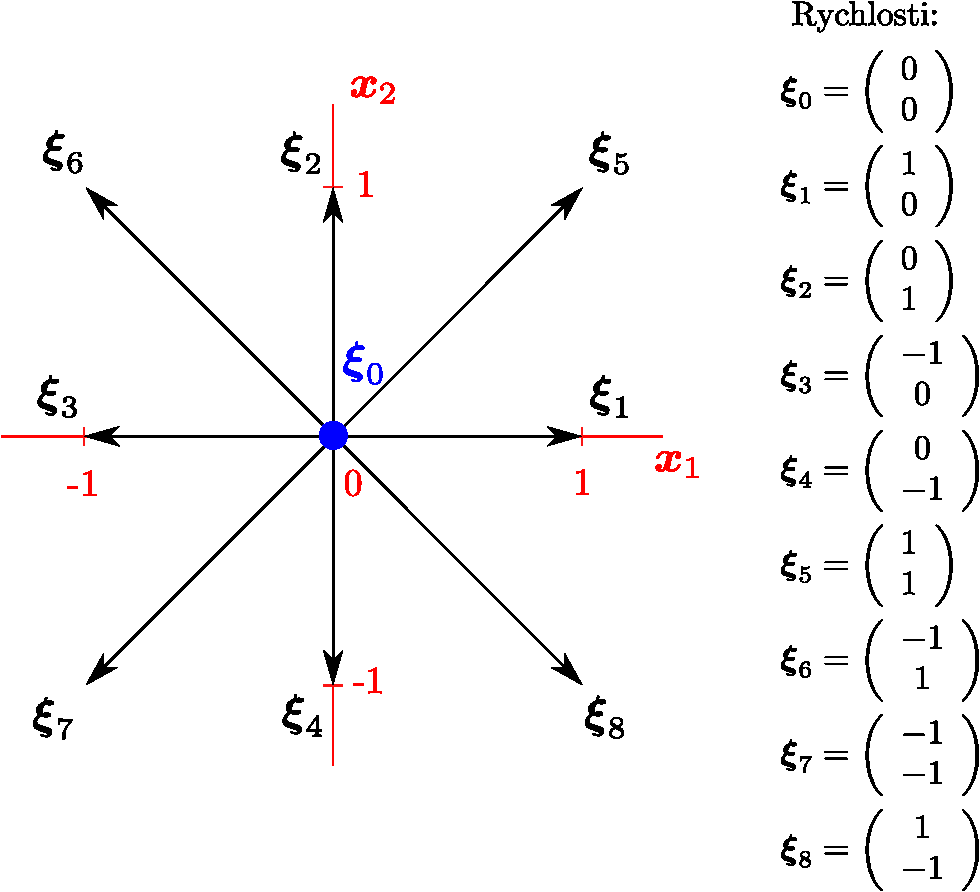
\includegraphics[width=.71\textwidth]{Images/d2q9.pdf}
	\caption{Geometrické znázornění rychlostního modelu D2Q9.}
	\label{fig:d2q9}
\end{figure}

\section{Bezrozměrnost a diskretizace}
Výpočetní oblast $ (0 ; L_1) \times(0 ; L_2)$, kde $ L_1 $ \si{[m]}, $ L_2 $ \si{[m]} jsou její rozměry, diskretizujeme ekvidistantní sítí s prostorovým krokem $ \Delta l $ \si{[m]}. Časový interval pak dělíme rovnoměrně s časovým krokem~$ \Delta t $~\si{[s]}.

V rámci LBM je pak běžné pracovat s bezrozměrnými veličinami namísto původních fyzikálních, důvody jsou diskutovány např. v \cite{Kruger}. Dále proto představíme základní převodní vztahy při přechodu~k berozměrnému systému jednotek. Definujeme také mřížku, použitou k diskretizaci oblasti v rámci LBM a popíšeme diskretizovanou Boltzmannovu transportní rovnici.

\subsection{Přechod k bezrozměrným jednotkám}
Jak bylo zmíněno, v rámci LBM je z hlediska použitelnosti a numerické přesnosti výhodné uvažovat všechny veličiny jako bezrozměrné. Přejdeme od fyzikálních jednotek k bezrozměrným mřížkovým jednotkám. Zdůrazněme, že fyzikální principy zůstavají platné nezávisle na volbě soustavy jednotek. Přechod mezi soustavami jednotek lze provést s použitím zákona podobnosti pro dynamiku tekutin, v~kterém je pro ekvivalenci soustav požadováno, aby hodnota relevantních bezrozměrných veličin zůstala zachována \cite{Kruger}. Takovou bezrozměrnou veličinou, kterou lze při přechodu mezi soustavami využít, je např.~Reynoldsovo číslo \eqref{Re}.

V následujících konverzních vztazích jsou všechny veličiny v mřížkových jednotkách označeny pravým horním indexem $ L $. Lze ukázat \cite{Kruger}, že platí
\begin{eqnarray}
	l^{L}_0 &=& \dfrac{l_{0}}{\Delta l},\\[5pt]
	t^{L}_0 &=& \dfrac{t_{0}}{\Delta t},\\[5pt]
	\nu^L &=& \nu \dfrac{\Delta t}{\Delta l^{2}} 	,\\[5pt]
	u^{L}_{i} &=& \dfrac{\Delta t}{\Delta l} u_{i}, \ i \in \{1, 2, 3\}.
\end{eqnarray}
Hodnoty charakteristické délky, charakteristického času a charakteristické rychlosti volíme v souladu s danou fyzikální úlohou. Jako $ l_{0} $ nejčastěji volíme rozměr výpočetní oblasti nebo překážky. Detaily odvozeních výše uvedných konverzních vztahů lze najít v \cite{Kruger}.

Podotkněme, že z konverzního vztahu pro kinematickou viskozitu můžeme vidět, že pro danou síť s~prostorovým krokem $ \Delta l $ je časový krok $ \Delta t $ svázán s~hodnotou $ \nu^L $.

Pro jednoduchost budeme v rámci této práce pro prostorový krok $ \Delta l ^L $ a časový krok $ \Delta t ^L $ v mřížkových jednotkách uvažovat $ \Delta l ^L  =  \Delta t ^L = 1$. Zdůrazněme, že v této kapitole budeme dále pracovat výhradně s veličinami v mřížkových jednotkách, upustíme tedy od rozlišování pomocí speciálního označení a nebudeme používat horní index $ L $, ačkoliv budeme dále bezrozměrný popis uvažovat.

\subsection{Výpočetní oblast a diskrétní mřížka}
V této části již implicitně předpokládáme, že všechny veličiny jsou uvedené v mřížkovým jednotkách, tedy $ \Delta l $, resp. $ \Delta t $ dále značí bezrozměrný prostorový krok, resp. časový krok. Uvažujeme obdélníkovou výpočetní oblast $ \Omega \subset \mathbb{R}^2$, viz sekce \ref{pred}. Tuto oblast v rámci LBM diskretizujeme pomocí ekvidistantní mřížky

\begin{subequations}\label{eq:oblast}
	\begin{eqnarray}
	\hat{\Omega} &=& \big\{ \vec{x}_{i,j} = (i \Delta l,\,j \Delta l)^T \, \big| \ i \in \{1, \dots, N_{1} - 1\}, j \in \{1, \dots, N_{2} - 1 \} \, \big\},\\[4pt]
	\overline{\hat{\Omega}} &=& \big\{ \vec{x}_{i,j} = (i \Delta l,\,j \Delta l)^T \, \big| \ i \in \{0, \dots, N_{1} \}, j \in \{0, \dots, N_{2} \} \, \big\},
	\end{eqnarray}
\end{subequations}
kde $ N_{1}$ [-] , resp. $ N_{2} $ [-], značí počet uzlových bodů ve směru $ x_1 $, resp. ve směru $x_2$.

Hranici oblasti $ \Omega $ budeme značit $ \partial \Omega $ a budeme ji chápat jako uzávěr disjunktního sjednocení jednotlivých částí 
\begin{equation}\label{eq:border decomposition}
\partial \Omega = \overline{\partial \Omega_{\mathrm{W}} \cup \partial \Omega_{\mathrm{E}} \cup \partial \Omega_{\mathrm{N}} \cup \partial \Omega_{\mathrm{S}}},
\end{equation}
kde významy $ \partial \Omega_{\mathrm{W}} , \partial \Omega_{\mathrm{E}} , \partial \Omega_{\mathrm{N}} $ a $ \partial \Omega_{\mathrm{S}}$ jsou znázorněny na obr. \ref{fig:oblast}. Dále budeme uvažovat diskretizaci hranice výpočetní oblasti jako
\begin{equation}\label{eq:border}
\partial\hat{\Omega} = \overline{\hat{\Omega}} \, \backslash \, \hat{\Omega},
\end{equation}
přičemž odpovídající části diksrétní hranice budeme značit $ \partial \hat{\Omega}_{\mathrm{W}} , \partial \hat{\Omega}_{\mathrm{E}} , \partial \hat{\Omega}_{\mathrm{N}} $ a $ \partial \hat{\Omega}_{\mathrm{S}}$.
\begin{figure}[H]
	\centering
	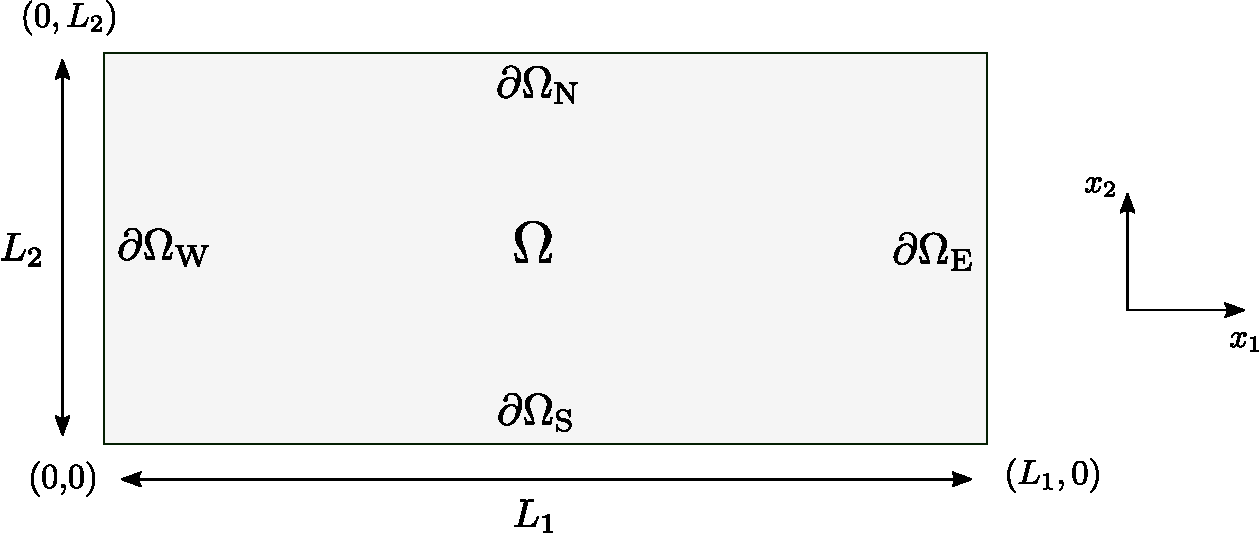
\includegraphics[width=0.85\textwidth]{Images/oblast.pdf}
	\caption{Schematické znázornění výpočetní oblasti $ \Omega $ a její hranice $ \partial \Omega $. Význam disjunktních částí hranice $ \partial \Omega$ je určen přiřazením daných označení k části hranice oblasti tak, jako je tomu na obrázku.}  
	\label{fig:oblast}
	\vspace{1.8mm}
\end{figure}

Časový interval, na kterém budeme danou úlohu vyšetřovat, budeme značit $ \mathcal{I} $ (viz sekce \ref{pred}), přičemž $ \mathcal{I} = \langle 0, T \rangle,$ kde $ T > 0$. Interval $ \mathcal{I} $ diskretizujeme jako
\begin{equation}\label{eq:timediscrete}
\hat{\mathcal{I}} = \left\{ t_{i} =i\dfrac{T}{N_t} \ \Big| \ i \in \big\{0, \dots, N_{t} \big\} \right\},
\end{equation}
kde $ N_t $ představuje počet diskrétních časových kroků určených pro diskretizaci intervalu $ \mathcal{I} $.

\subsection{Diskrétní Boltzmannova transportní rovnice}
Podotkněme, že při použití modelu D2Q9 budeme dále pracovat se sadou distribučních funkcí
\begin{equation}\label{eq:ddfs}
	\left\{ f_k (\vec{x}, t)\, \big| \, k = 0, 1, \dots, 8 \, \right\} , \ \forall \vec{x} \in \hat{\Omega}, \ \forall t \in \hat{\mathcal{I}},
\end{equation}
kde indexy odpovídají označení směrů u mikroskopických rychlostí v obr.~\ref{fig:d2q9}.

Lze ukázat, že diskretizací rovnice \eqref{eq:BTR} dostaneme tvar
\begin{equation}\label{eq:BTRdiscrete}
f_{k}\left(\vec{x}+\Delta t \vec{\xi}_{k}, t+\Delta t \right) =
f_{k}(\vec{x}, t) + \mathcal{C}_{k}(\vec{x}, t) + \mathcal{S}_{k}(\vec{x}, t), \hspace{2.5mm} k \in \{0, \dots, q-1 \}, \ \forall \vec{x} \in \hat{\Omega}, \ \forall t \in \hat{\mathcal{I}},
\end{equation}
kde $ \mathcal{C}_{k} $ představuje diskrétní kolizní operátor a $ \mathcal{S}_{k} $ je diskrétní silový člen, jejichž podoba závisí na zvoleném typu mřížkové Boltzmannovy metody a je dále diskutována v sekci \ref{kol}. Detaily odvození diskrétní formy Boltzmannovy transportní rovnice jsou k nahlédnutí v \cite{Kruger}.

Dále můžeme zavést tzv. postkolizní distribuční funkce $ f^{*}_{k} $ vztahem
\begin{equation}\label{eq:fstar}
f^{*}_{k}(\vec{x}, t) = f_{k}(\vec{x}, t) + \mathcal{C}_{k}(\vec{x}, t) + \mathcal{S}_{k}(\vec{x}, t), \hspace{2.5mm} k \in \{0, \dots, q-1 \}, \ \forall \vec{x} \in \hat{\Omega}, \ \forall t \in \hat{\mathcal{I}}.
\end{equation}
Pomocí $ f^{*}_{k} $ můžeme vyjádřit \eqref{eq:BTRdiscrete} ve tvaru
\begin{equation}\label{eq:collision}
f_{k}\left(\vec{x}+\Delta t \vec{\xi}_{k}, t+\Delta t\right) = f^{*}_{k}(\vec{x}, t), \hspace{2.5mm} k \in \{0, \dots, q-1 \}, \ \forall \vec{x} \in \hat{\Omega}, \ \forall t \in \hat{\mathcal{I}},
\end{equation}
což lze vnímat jako explicitní předpis pro výpočet distribučních funkcí.

\subsection{Makroskopické veličiny}\label{macro}
Na závěr uvedeme vztahy pro výpočet některých makroskopických veličin. Některé z těchto vztahů lze odvodit s pomocí procesu diskretizace z obecných vztahů \ref{eq:macroscopic basic} \cite{Kruger}. Vztah pro výpočet hustoty, hybnosti a tlaku má tvar

\begin{subequations}\label{macroeq}
	\begin{eqnarray}
	\label{rho}
	\rho &=& \sum_{k=0}^{q-1} f_{k},\\[3pt]
	\rho \vec{u} &=& \sum_{k=0}^{q-1} f_{k} \vec{\xi_{k}} + \rho \dfrac{\Delta t}{2} \vec{g},\\[3pt]
	p &=& p_0 + c_{s}^{2} (\rho - \rho_0),
	\end{eqnarray}
\end{subequations}
kde $ p_0 $ \si{[-]} je bezrozměrná referenční hodnota tlaku, $ c_s $ \si{[-]} je bezrozměrná (mřížková) rychlost zvuku a $ \rho_0 $ je bezrozměrná referenční hodnota hustoty. Pro $ c_s $ v použitém modelu D2Q9 platí $ c_s = \frac{1}{\sqrt{3}} $. Dále uvažujeme volbu $ \rho_0 = 1 $. Podrobný popis výpočtu makroskopických veličin je uveden v \cite{Kruger}.

\section{Algoritmus LBM}\label{algoritmus LBM}
Algoritmus LBM lze shrnout do několika bodů:
\begin{enumerate}
	\item \textbf{Inicializace} počátečních podmínek v mřížce, diskutováno v sekci \ref{pocatecni a okrajove podminky}.
	\item \textbf{Cyklus} končící splněním podmínky ukončení, která je zadána uživatelem.
	\begin{enumerate}
		\item \textbf{Šíření} (anglicky \textit{streaming}) postkolizních distribučních funkcí $ f^{*}_{k} $  v příslušných směrech $ \vec{\xi_{k}} $.
		\item \textbf{Výpočet makroskopických veličin} pomocí vztahů \eqref{macroeq}.
		\item \textbf{Kolize} (anglicky \textit{collision}), kdy dochází k výpočtu postkolizního stavu distribuční funkce pomocí \eqref{eq:collision} a \textbf{vyřešení okrajových podmínek} diskutovaných v sekci \ref{pocatecni a okrajove podminky}.
	\end{enumerate}
	\item \textbf{Konec algoritmu.}
\end{enumerate}
Vývojový diagram LBM je k nahlédnutí na obr. \ref{fig:algo}.
\begin{figure}[h]
	\centering
	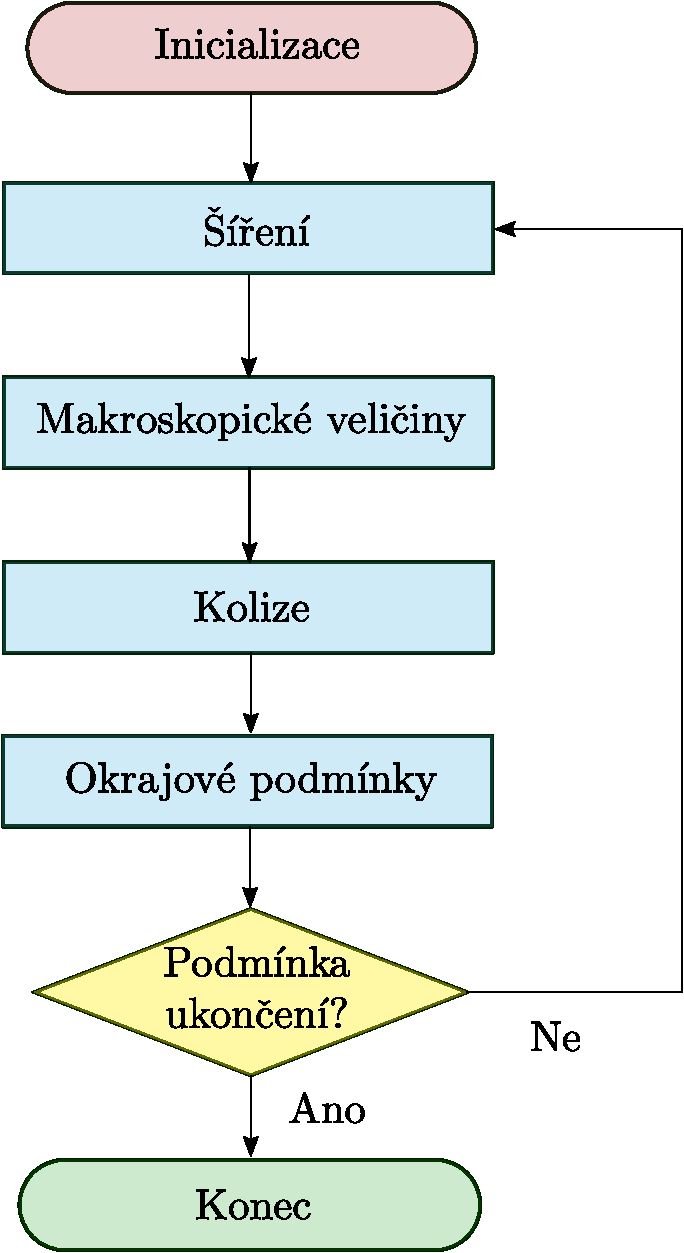
\includegraphics[width=0.3\textwidth]{Images/algoritmus.pdf}
	\caption{Vývojový diagram algoritmu LBM.}
	\label{fig:algo}
\end{figure}


\section{Kolizní operátory}\label{kol}
V diskretizované Boltzmannově transportní \eqref{eq:BTRdiscrete} rovnici vystupuje diskrétní kolizní operátor $ \mathcal{C}_{k} $, jehož zvolená podoba určuje různé typy LBM. Existuje více možností volby  $ \mathcal{C}_{k} $, můžeme pak rozlišit např. varianty SRT-LBM~\cite{GeierCuLBM}, MRT-LBM~\cite{MRT}, CLBM~ \cite{GeierCLBM}, ELBM~\cite{ELBM} nebo CuLBM~\cite{GeierCuLBM}. V této práci se omezíme pouze na využití typu kaskádové LBM (CLBM), který stručně popíšeme v rámci námi uvažovaného rychlostního modelu D2Q9. Detailní odvození metody CLBM lze najít např. v \cite{GeierCLBM}.

Definujme nejdříve diskrétní centrální momenty jako
\begin{equation}\label{eq:centralmoment} 
%\kappa_{(\alpha_{1}, \alpha_{2})} = 
\sum_{k=0}^{8} f_{k} (\xi_{k,1}  - u_{1})^{\alpha_{1}} (\xi_{k,2}  - u_{2})^{\alpha_{2}},
\end{equation}
kde $ \vec{\alpha} = (\alpha_{1}, \alpha_{2}) \in \mathbb{N}^2_{0}$.
%
%Za předpokladu $ \vec{g} = \vec{0}$ zjevně platí
%\begin{subequations}\label{eq:central moments}
%	\begin{eqnarray}
%	k_{(0,0)} &=& \rho,\\[3pt]
%	k_{(1,0)} &=& \sum_{k=0}^{8} f_{k} (\xi_{k,1} - u_{1}) = 0,\\[3pt]
%	k_{(0,1)} &=& \sum_{k=0}^{8} f_{k} (\xi_{k,2} - u_{2}) = 0.
%	\end{eqnarray}
%\end{subequations}

Důležitým aspektem CLBM je, že kolizní krok zmíněný v sekci \ref{algoritmus LBM} je v rámci této metody realizován v prostoru diskrétních centrálních momentů distribučních funkcí, což zlepšuje numerickou stabilitu tohoto schématu \cite{GeierCLBM}. Kolizní operátor CLBM je konstruovaný tak, že každý z centrálních momentů spěje do rovnovážného stavu nezávisle na ostatních centrálních momentech. CLBM využívá při použití rychlostního modelu D2Q9 devět relaxačních parametrů, které označíme jako $ \tau_{0}, \dots, \tau_{8} $ \cite{DP-PE}. 

Matici přechodu z prostoru distribučních funkcí do prostoru momentů označíme $ \mathbf{K} $. Konkrétní tvar báze prostoru momentů distribučních funkcí a matice $ \mathbf{K} $ lze najít např. v \cite{DP-PE}. Podotkněme, že z volby báze toho prostoru se pak odvíjí i tvar transformační matice $ \mathbf{K} $. Jak bylo zmíněno, ke kolizi dochází v rámci schématu CLBM v prostoru centrálních momentů, diskrétní kolizní operátor tedy můžeme psát ve tvaru
\begin{equation}\label{eq:clbm collision}
	\mathcal{C}_k = (\mathbf{K} \vec{v})_k, \ k \in \{0, \dots, 8 \},
\end{equation}
kde pro jednoznačné určení kolize musí být určen tvar $ \vec{v} = (v_0, \dots, v_8)$. Z tvaru matice $ \mathbf{K} $ lze ukázat, že první tři centrální momenty odpovídají hustotě a složkám hybnosti. Hybnost a složky rychlosti se však vlivem kolize nemění, z toho důvodu je tedy pro jednoznačné určení kolize nutné určit pouze složky $ v_3, \dots, v_8 $ a zbylé složky můžeme volit nulové. Odvození tvaru $ v_3, \dots, v_8 $	 lze najít např. v \cite{GeierCLBM, DP-PE}. Dále je nutné určit tvar diskrétního operátoru zdrojových členů $ \mathcal{S}_k, \, k \in \{ 0, \dots, 8\} $ - odvození lze opět najít např. v \cite{GeierCLBM, DP-PE}.


%S pomocí těchto relaxačních časů definujeme diagonální matici 
%\begin{equation}\label{eq:matrixS}
%\mathbf{S} = \mathrm{diag} \, \Bigg( \frac{\Delta t}{\tau_{0}}, \frac{\Delta t}{\tau_{1}}, \dots, \frac{\Delta t}{\tau_{8}} \Bigg)
%\end{equation}
%a vektor $ \vec{f} = \left(f_{0}, f_{1}, \dots, f_{8} \right)^T$  \cite{GeierCLBM}. Kolizní operátor má pak tvar
%\begin{equation}\label{eq:collision operator Ck}
% \mathcal{C}_{k} = \mathbf{K^{-1}}\mathbf{S}(\vec{\kappa}^{\mathrm{eq}} - \vec{\kappa}),
%\end{equation}
%kde $ \mathbf{K} $ je matice přechodu z prostoru distribučních funkcí do prostoru centrálních momentů, $ \vec{\kappa} $ je vektor centrálních momentů splňující $ \vec{\kappa} =  \mathbf{K} \vec{f} $ a $ \vec{\kappa}^{\mathrm{eq}} $ je vektor představující rovnovážné centrální momenty distribučních funkcí \cite{GeierCLBM}. Matici přechodu $ \mathbf{K} $ volíme tak, aby vektor $ \vec{\kappa} $ splňoval
%\begin{equation}\label{eq:kappa}
%\vec{\kappa} = (k_{(0,0)}, k_{(1,0)}, k_{(0,1)}, k_{(1,1)}, k_{(2,0)} + k_{(0,2)}, k_{(2,0)} - k_{(0,2)}, k_{(2,1)}, k_{(1,2)} , k_{(2,2)})^T,
%\end{equation}
%a aby platilo
%\begin{equation}\label{eq:kappaeq}
%\vec{\kappa}^{\mathrm{eq}} = (\rho, 0, 0, 0, 2 \rho c^{2}_{s}, 0, 0, 0, \rho c^{4}_{s})^T.
%\end{equation}
Prozkoumejme dále tvar relaxačních parametů $ \tau_{0}, \dots, \tau_{8}$. Platí, že $ \nu $ je závislá na relaxačních parametrech $ \tau_{4} $ a $ \tau_{5} $. S využitím předpokladu izotropie viskozity \cite{DP-PE} můžeme volit
\begin{equation}
\tau_{4} = \tau_{5} = \tau,
\end{equation}
kde hodnota $ \tau $ splňuje
\begin{equation}\label{eq:tauclbm}
\nu = c^{2}_{s} \, \Bigg( \tau  - \frac{\Delta t}{2} \Bigg).
\end{equation}
Další relaxační parametry lze volit ke zlepšení numerické stability a volíme je dle \cite{GeierCLBM} jako
\begin{equation}
\tau_{3} = \tau_{6} = \tau_{7} = \tau_{8} = 1,
\end{equation}
přičemž na hodnotách $ \tau_{0}, \tau_{1} $ a $ \tau_{2} $ z důvodu tvaru složek vektoru $\vec{v}$ nezáleží.

\section{Počáteční a okrajové podmínky}\label{pocatecni a okrajove podminky}

Vhodná volba počátečních a okrajových podmínek, která je v souladu se zkoumanou úlohou, je nedílnou součástí následné numerické simulace. Z důvodu specifického mezoskopického popisu tekutiny v rámci LBM je volbě počátečních a okrajových podmínek později použitých v praktické části práce nutné věnovat zvýšenou pozoronost, a proto jsou dále použité počáteční a okrajové podmínky podrobněji popsány.

\subsection{Počáteční podmínka}\label{pocatecni podminka}
Uvažujme nyní oblast definovanou vztahy \eqref{eq:oblast}. K nastavení počáteční podmínky využijeme rovnovážnou distribuční funkci $ f^{\mathrm{eq}} $, která má tvar 
\begin{equation}\label{eq:feq}
f^{\mathrm{eq}}_{k} = \rho w_{k} \, \Bigg(1 + \frac{\vec{\xi_{k}} \cdot \vec{u}}{c^{2}_{s}} + \frac{(\vec{\xi_{k}} \cdot \vec{u})^2}{2c^{4}_{s}} - \frac{\vec{u} \cdot \vec{u}}{2c^{2}_{s}} \Bigg)\, , \hspace{2mm} k \in \{0,\dots,q-1\},
\end{equation}
kde $ w_{k} $ představují váhy specifické pro vybraný rychlostní model, přičemž pro použitý model D2Q9 platí~\cite{Kruger}
\begin{align}\label{weighs}
\begin{split}
w_{0} &  = \dfrac{4}{9},\\[4pt]
w_{1} = w_{2} = w_{3} = w_{4} & = \frac{1}{9},\\[4pt]
w_{5} = w_{6} = w_{7} = w_{8} & = \frac{1}{36}.
\end{split}
\end{align}
Počáteční rozložení $ \rho $, resp. $ \vec{u} $, definujeme jako $ \rho _{\mathrm{ini}} $, resp. $ \vec{u} _{\mathrm{ini}} $. Poté pro každý uzel $ \vec{x} \in \hat{\Omega} $ v čase $ t=0 $ bude platit

\begin{equation}\label{eq:initial condition}
f^{}_{k} (\vec{x}, 0) = f^{\mathrm{eq}}_{k} (\rho _{\mathrm{ini}} (\vec{x}), \vec{u} _{\mathrm{ini}} (\vec{x})), \hspace{3mm} k \in \{0, 1, \dots q-1\}.
\end{equation}
V rámci tohoto přístupu nastavení počáteční podmínky předpokládáme, že nerovnovážná část distribučních funkcí $ f^{\mathrm{neq}}_{k} = f_{k} - f^{\mathrm{eq}}_{k}$ může být zanedbána a distribuční funkce mohou tak být aproximovány svou rovnovážnou částí. Značnou výhodou této volby aproximace počáteční podmínky je její následná jednoduchá implementace, a proto je v rámci této práce použita, byť existují i jiné, sofistikovanější, volby, viz např. \cite{PE}.

\subsection{Okrajové podímky}


\subsubsection{Bounce-back okrajová podmínka}\label{bounce-back}
První zmíněnou okrajovou podmínkou je bounce-back okrajová podmínka, konkrétně její varianta \textit{fullway}. Bounce-back okrajová podmínka se typicky používá na rozhraní tekutiny a pevné látky. Její výhoda je, že na rozhraní splňuje neklouzavou (anglicky \textit{no-slip}) okrajovou podmínku a že její implementace je přímočará. Princip bounce-back okrajové podmínky je takový, že na rozhraní dojde k myšlenému odrazu distribučních funkcí odpovídajích částicím s mikroskopickou rychlostí $ \vec{\xi_{k}} $ zpět do směrů, ze kterých se do daného uzlu dostaly s rychlostí $ \vec{\xi_{\bar{k}}} = -\vec{\xi_{k}}$.

Při použití této okrajové podmínky se rozhraní nachází v polovině vzdálenosti mezi uzly tekutiny a tělesa. Tato skutečnost nepůsobí problémy při modelování proudění okolo rovných zdí, které jsou rovnoběžné s použitou mřížkou. Pro zakřivené hranice nerovnoběžné s mřížkou však metoda bounce-back dává za vznik "schodovitému" \ tvaru hranice, a tedy neposkytuje vhodnou aproximaci skutečné pozice rozhraní, viz obr. \ref{fig:staircase}.

\begin{figure}[H]
	\centering
	\vspace{2mm}
	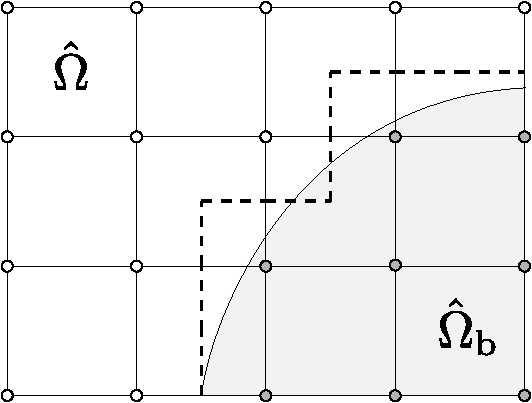
\includegraphics[width=0.37\textwidth]{Images/stairboundary.pdf}
	\vspace{2mm}
	\caption{"Schodovitý" \ tvar hranice vznikající při použití bounce-back okrajové podmínky.}
	\label{fig:staircase}
	\vspace{1.8mm}
\end{figure}


Fullway varianta bounce-back okrajové podmínky vyžaduje ke své realizaci a odražení hypotetických částic dva časové kroky. Během nich doputují částice až do uzlů pevné látky, kde je jejich směr následně v dalším kroku šíření obrácen, jak je schematicky znázorněno na obr. \ref{fig:bb}.

\begin{figure}[h]
	\centering
	\vspace{2mm}
	\hspace{7mm}
	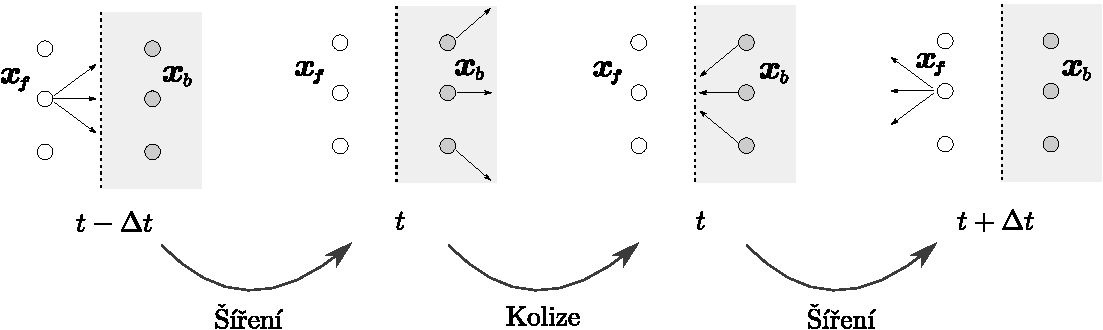
\includegraphics[width=0.9\textwidth]{Images/bb.pdf}
	\vspace{2.8mm}
	\caption{Schématické znázornění fullway bounce-back okrajové podmínky. Šipky představují směr šíření hypotetické částice, oblast s šedou barvou představuje pevné těleso a čárkovaná hranice odpovídá pozici rozhraní.}
	\label{fig:bb}
	\vspace{1.8mm}
\end{figure}


Podotkněme, že dále existuje \textit{halfway} varianta bounce-back okrajové podmínky, která ke své realizaci potřebuje pouze jeden časový krok, detaily lze najít např. v \cite{Kruger}. Nicméně v rámci této práce se omezíme pouze na využití varianty fullway.
 

\subsubsection{Interpolační okrajové podmínky}\label{interpolation bc}
Jak již bylo zmíněno, bounce-back okrajová podmínka nereflektuje správným způsobem zakřivenou hranici tělesa. Vhodnější volbou okrajové podmínky pro rozhraní tekutiny a tělesa se zakřivenou hranicí jsou tzv. interpolační okrajové podmínky.

Obě dále zmíněné interpolační okrajové podmínky využívají k výpočtu distribučních funkcí lineární nebo kvadratickou interpolaci, při níž je použit bezrozměrný parametr $ \Theta $ definovaný vztahem
\begin{equation}\label{eq:q}
\Theta = \frac{\norm{\vec{x}_{f{_A}}-\vec{x}_w}}{\norm{\vec{x}_{f{_A}}-\vec{x}_b}},
\end{equation}
kde $ \vec{x}_{f{_A}} $ je uzel tekutiny na hranici, $ \vec{x}_b =  \vec{x}_{f{_A}} + \Delta t \vec{\xi_{k}}$ je uzel pevné překážky, dále $ \vec{x}_w$ se nachází na skutečné hranici objektu tak, jak je ilustrováno na obr. \ref{fig:bouz}. Pro pozdější využití navíc dále zavádíme body \mbox{$ \vec{x}_{f{_B}} = \vec{x}_{f{_A}} + \Delta t \vec{\xi_{\bar{k}}} \,$} a $\,  \vec{x}_{f{_C}} = \vec{x}_{f{_A}} + 2\Delta t \vec{\xi_{\bar{k}}}  $, kde index $ \bar{k} $ splňuje $ \vec{\xi_{\bar{k}}} = -\vec{\xi_{k}}$. Jejich význam je společně s významem vzdáleností použitých ve výpočtu parametru $ \Theta $ znázorněn na obr. \ref{fig:bouz2}. Podotkněme, že na hranici tělesa dále uvažujeme no-slip podmínku.
\begin{figure}[H]
	\centering
	\begin{subfigure}{0.95\textwidth}
		\centering
		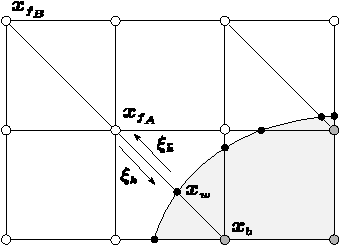
\includegraphics[width=0.45\textwidth]{Images/bouzidi.pdf}
		\caption{Ilustrace významu bodů $ \vec{x}_{f{_A}}, \vec{x}_w, \vec{x}_b$. Černé body na skutečné hranici tělesa představují pozice všech bodů $ \vec{x}_w$, které slouží k výpočtu parametru $ \Theta $ pro různé body tekutiny $ \vec{x}_{f{_A}} $ pro různé směry.}
		\label{fig:bouz}
	\end{subfigure}%
	\\[10pt]
	\begin{subfigure}{0.95\textwidth}
		\centering
		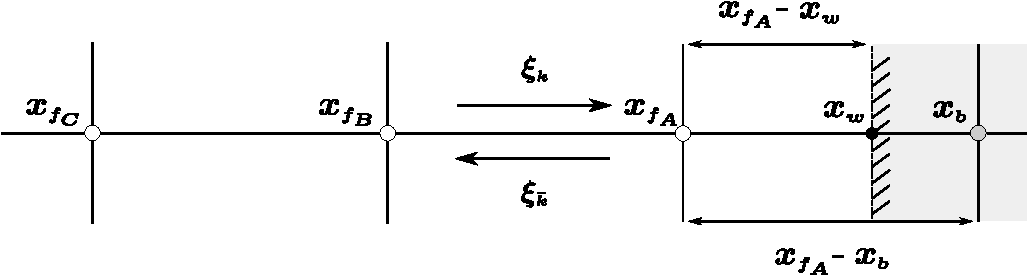
\includegraphics[width=0.85\textwidth]{Images/bouzidi2.pdf}
		\caption{Ilustrace významu bodů $ \vec{x}_{f{_B}} $ a $ \vec{x}_{f{_C}} $ a vzdáleností vyskytujících se ve výpočtu parametru $ \Theta $.}
		\label{fig:bouz2}
	\end{subfigure}
	\vspace{3mm}
	\caption{Schématické znázornění významu členů využitých v rámci interpolačních okrajových podmínek. Šedá oblast představuje oblast tělesa.}
	\label{fig:lattice}
\end{figure}

Jako první představíme interpolační okrajovou podmínku navrženou M. Bouzidim a kol. (dále jen Bouzidiho okrajová podmínka) v \cite{Bouzidi2001}. Popíšeme proces využitý k odvození jejího tvaru při lineární interpolaci.

Uvažujme nejdříve $ \Theta \geq \frac{1}{2} $, tedy případ, kdy se skutečná hranice nachází blíže bodu $ \vec{x}_b $. Myšlená částice v $ \vec{x}_{f{_A}} $ pohybující se s rychlostí $ \vec{\xi_{k}} $ v čase $ t $ se od stěny odrazí v čase $ t + \Theta \Delta t$ v hraničním bodě $ \vec{x}_w $ s opačnou rychlostí $ \vec{\xi_{\bar{k}}} $. Po uplynutí dalšího časového úseku $ (1 - \Theta ) \Delta t $, tj. v čase $ t + \Delta t$ se částice bude nacházet v~bodě $ \vec{x}_t $, pro který platí
\begin{equation}
	\vec{x}_t = \vec{x}_f + (2\Theta - 1)\Delta t \vec{\xi}_{k}.
\end{equation}
Platí tedy $ f_{\bar{k}} (\vec{x}_t, t + \Delta t) = f^{*}_k ( \vec{x}_{f{_A}}, t)$. Schéma tohoto odrazu je k nahlédnutí na obr. \ref{fig:interp1}. Hodnota $ f_{\bar{k}} (\vec{x}_t, t + \Delta t)$ společně se známou hodnotou $ f_{\bar{k}} ( \vec{x}_{f{_B}}, t) = f^{*}_{\bar{k}} ( \vec{x}_{f{_A}}, t)$ je pak lineárně interpolována a tím je získána hodnota $ f_{\bar{k}}\left(\vec{x}_{f{_A}}, t+\Delta t\right) $.

Dále uvažejme $ \Theta < \frac{1}{2} $, tedy případ, kdy se skutečná hranice nachází blíže bodu $ \vec{x}_{f_A} $. Pro interpolaci využijeme bod
\begin{equation}
\vec{x}_t = \vec{x}_f + (1 - 2\Theta)\Delta t \vec{\xi}_{\bar{k}}.
\end{equation}
Myšlená částice v $ \vec{x}_{t} $ pohybující se s rychlostí $ \vec{\xi_{k}} $ v čase $ t $ se od stěny odrazí v čase $ t + (1 - \Theta) \Delta t$ v bodě $ \vec{x}_w $ s opačnou rychlostí $ \vec{\xi_{\bar{k}}} $. Za další časový úsek $ \Theta \Delta t $ se bude vyskytovat v bodě $ \vec{x}_{f{_A}} $. Platí tedy $ f^{*}_{k} (\vec{x}_t, t) = f_{\bar{k}} (\vec{x}_{f{_A}}, t + \Delta t)$. Schéma tohoto odrazu je k nahlédnutí na obr. \ref{fig:interp2}. Hodnotu $ f^{*}_{k} (\vec{x}_t, t) $ získáme lineární interpolací hodnot $ f^{*}_{k} (\vec{x}_{f_A}, t) $ a $ f^{*}_{k} (\vec{x}_{f_B}, t) $.
\begin{figure}[H]
	\centering
	\begin{subfigure}{0.5\textwidth}
		\centering
		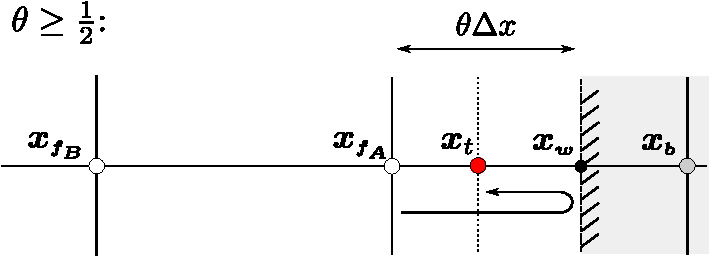
\includegraphics[width=0.95\textwidth]{Images/interpolace1.pdf}
		\vspace{2mm}
		\caption{Ilustrace odrazu částice při hodnotě $ \Theta \geq \frac{1}{2} $.}
		\label{fig:interp1}
	\end{subfigure}%
	\begin{subfigure}{0.5\textwidth}
		\centering
		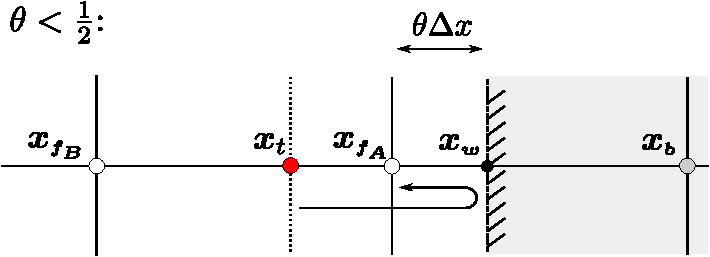
\includegraphics[width=0.95\textwidth]{Images/interpolace2.pdf}
		\vspace{2mm}
		\caption{Ilustrace odrazu částice při hodnotě $ \Theta < \frac{1}{2} $.}
		\label{fig:interp2}
	\end{subfigure}
	\caption{Schématické znázornění konstrukce použité při odvození Bouzidiho okrajové podmínky za použití lineární interpolace.}
	\label{fig:interp}
\end{figure}

Shrneme-li výsledky lineární interpolace pro oba zmínené případy hodnoty parametru $ \Theta $, má Bouzidiho okrajová podmínka tvar
\begin{align}\label{eq:lbouz}
\begin{split}
\Theta &< \dfrac{1}{2}: \hspace{7mm} 
f_{\bar{k}}\left(\vec{x}_{f{_A}}, t+\Delta t\right) = 2 \Theta f_{k}^{*}\left(\vec{x}_{f{_A}}, t\right)+(1-2 \Theta) f_{k}^{*}\left(\vec{x}_{f{_B}}, t\right),\\[6pt]
\Theta &\geq \dfrac{1}{2}: \hspace{7mm} f_{\bar{k}}\left(\vec{x}_{f{_A}}, t+\Delta t\right) = \frac{1}{2 \Theta} f_{k}^{*}\left(\vec{x}_{f{_A}}, t\right)+\frac{2 \Theta-1}{2 \Theta} f_{\bar{k}}^{*}\left(\vec{x}_{f{_A}}, t\right).
\end{split}
\end{align}

Jak bylo zmíněno, k odvození lze použít i kvadratickou interpolaci. Při použití kvadratické interpolace má Bouzidiho okrajová podmínka tvar
\begin{align}\label{eq:qbouz}
\begin{split}
\Theta &< \dfrac{1}{2}: \hspace{3mm} 
f_{\bar{k}}\left(\vec{x}_{f{_A}}, t+\Delta t\right) =
\Theta \left( 1 + 2\Theta \right) f_{k}^{*}\left(\vec{x}_{f{_A}}, t\right)+
(1-4 \Theta^2) f_{k}^{*}\left(\vec{x}_{f{_B}}, t\right)-
\Theta \left( 1 - 2\Theta \right) f_{k}^{*}\left(\vec{x}_{f{_C}}, t\right),\\[6pt]
\Theta &\geq \dfrac{1}{2}: \hspace{3mm}
f_{\bar{k}}\left(\vec{x}_{f{_A}}, t+\Delta t\right) =
\frac{1}{\Theta \left(2 \Theta + 1\right)} f_{k}^{*}\left(\vec{x}_{f{_A}}, t\right) +
\frac{2\Theta - 1}{\Theta} f_{\bar{k}}^{*}\left(\vec{x}_{f{_A}}, t\right) -
\frac{2\Theta - 1}{2 \Theta + 1} f_{\bar{k}}^{*}\left(\vec{x}_{f{_B}}, t\right).
\end{split}
\end{align}

Bouzidiho interpolační schéma používá dva různé vzorce na základě hodnoty parametru $ \Theta $. V~\cite{Yu2003}~však bylo odvozeno interpolační schéma, které oba případy sjednocuje v jeden společný tvar pro všechny hodnoty~$ \Theta $. Okrajovou podmínku využívající toto schéma nazýváme sjednocená okrajová podmínka (anglicky \textit{unified interpolation scheme}). Opět lze pro její odvození využít lineární nebo kvadratickou interpolaci.
Při použití lineární interpolace má sjednocená okrajová podmínka tvar
\begin{equation}\label{eq:luni}
f_{\bar{k}}\left(\vec{x}_{f{_A}}, t+\Delta t\right)= \frac{1}{1+\Theta} \, \Big[ \Theta f_{k}\left(\vec{x}_{f{_A}}, t\right)+(1-\Theta) {f}_{k}\left(\vec{x}_{f{_B}}, t\right) +\Theta {f}_{\bar{k}}\left(\vec{x}_{f{_A}}, t\right) \Big].
\end{equation}
Použitím kvadratické interpolace získáme pro sjednocenou okrajovou podmínku tvar
\begin{align}\label{eq:quni}
\begin{split}
f_{\bar{k}}\left(\vec{x}_{f_A}, t+\Delta t\right)=& \,
\frac{1}{(1+\Theta)(2+\Theta)} \, \Big[\Theta(1+\Theta) {f}_{k}\left(\vec{x}_{f{_A}}, t\right)+2\left(1-\Theta^{2}\right) {f}_{k}\left(\vec{x}_{f{_B}}, t\right)
\\&-\Theta(1-\Theta) {f}_{k}\left(\vec{x}_{f{_C}}, t\right)+2 \Theta(2+\Theta) {f}_{\bar{k}}\left(\vec{x}_{f{_A}}, t\right) 
-\Theta(1+\Theta) {f}_{\bar{k}}\left(\vec{x}_{f{_B}}, t\right) \Big].
\end{split}\end{align}

\subsubsection{Rovnovážná okrajová podmínka}\label{equilibrium bc}
Jednou z možností jak aproximovat neznáme hodnoty distribučních funkcí v krajních uzlových bodech oblasti je pomocí rovnovážné distribuční funkce jako \cite{PE}

\begin{equation}
	f_i(\vec{x}, t)=f_{i}^{\text{(eq)}}(\rho(\vec{x}, t), \vec{u}(\vec{x}, t)), \hspace{2mm}  \forall k \in \{0,\dots,q-1\}, \forall t \in \hat{\mathcal{I}}.
\end{equation}

Výhodou této aproximace je její snadná implementace, nevýhodou je zanedbání nerovnovážné části distribuční funkce \cite{PE}.

\subsubsection{Momentová okrajová podmínka}\label{moment based bc}

Momentová okrajová podmínka (anglicky \textit{moment-based boundary condition}) představuje způsob, jak na hranicích oblasti předepsat okrajovou podmínku na základě znalosti příslušných makroskopických momentů, s pomocí nichž a známých hodnot distribučních funkcí jsou zbylé, neznámé, distribuční funkce jednoznačně vyjádřitelné. Detaily odvození této okrajové podmínky lze najít v \cite{PE}.

Při použití momentové okrajové podmínky je předpokládána znalost diskrétních obecných momentů definovaných jako
\begin{equation}\label{eq:raw moments}
m_{(\alpha_{1}, \alpha_{2})} = \sum_{k=0}^{q-1} f_{k} \xi^{\alpha_{1}}_{k,1} \xi^{\alpha_{2}}_{k,2},
\end{equation}
kde $ \vec{\alpha} = (\alpha_{1}, \alpha_{2}) \in \mathbb{N}^2_{0}$.

Podobně jako tomu bylo pro centrální momenty v sekci \ref{kol}, lze zavést matici přechodu z prostoru distribučních funkcí do prostoru obecných momentů. Tuto matici budeme značit $ \mathbf{M} $, její konkrétní podobu lze najít např. v \cite{LBMAT}. Jelikož je $ \mathbf{M} $ regulární, lze na základě obecných momentů a známých hodnot distribučních funkcí vyjádřit libovolný počet neznámých distribučních funkcí. Pro výpočet hustoty lze využít hodnot známých distribučních funkcí a zadané rychlosti, naopak pro výpočet rychlosti použijeme známe distribuční funkce a zadanou hustotu.

Podotkněme, že z charakteru momentové okrajové podmínky vyplývá, že vztahy pro výpočet neznámých distribučních funkcí musí být odvozeny zvlášť pro každou požadovanou množinu těchto neznámých - v rámci modelu D2Q9 to znamená odvození pro 4 různé strany obdélníkové oblasti a 4 zbývající navzájem různé rohy této oblasti. Konkrétní vztahy pro každou tuto neznámou množinu distribučních funkcí 
%jsou k nahlédnutí v \cite{PE}.
jsou pro úplnost k nahlédnutí v příloze~\ref{priloha A}.


\section{Výpočet síly v LBM}\label{vypocet sily v LBM}

Existují dva standardní způsoby výpočtu síly v rámci LBM - metoda výměny hybnosti a metoda integrace tenzoru napětí, viz \cite{NASA}. Zde popíšeme pouze metodu integrace tenzoru napětí, detaily ohledně metody výměny hybnosti lze najít např. v \cite{NASA}. Dále uvažujme oblast~$ \Omega $, těleso $ \Omega_{\mathrm{b}} \subset \Omega $ a zkoumejme sílu, kterou tekutina v oblasti působí na těleso.

Metoda integrace tenzoru napětí (anglicky \textit{stress integration method}) je přímo založena na vztahu~\eqref{eq:stress_int}. Zapíšeme-li tento vztah v diskrétním tvaru, integrál přejde v sumu přes konečný počet bodů a~pro $ i $-tou složku síly $ \vec{F} $ dostaneme vztah ve tvaru
\begin{equation}\label{eq:sim}
{F}_{i}(t) = \sum_{\vec{x} \in  \partial \hat{\Omega}_{\mathrm{b}}}^{} \Delta s(\vec{x}) \sum_{j=1}^{2}  \sigma_{ij} (\vec{x}, t) \, n_{j} (\vec{x})  , \hspace{2mm} i \in \{ 1, 2 \},
\end{equation}
kde $ \Delta s(\vec{x}) $ \si{[-]} představuje bezrozměrnou náhradu diferenciálu $ \mathrm{d}S $ (viz~\eqref{eq:stress_int}) v bodě $ \vec{x}$, $ \sigma_{ij} (\vec{x}, t)$ představuje složky diskrétního úplného tenzoru napětí v bodě $ \vec{x} $ a v čase $ t $, dále pak $ \vec{n}(\vec{x}) $ představuje jednotkový vnější normálový vektor hranice tělesa v bodě $ \vec{x} \in \partial \hat{\Omega}_{\mathrm{b}}$. Upozorněme, že body z $ \partial \hat{\Omega}_{\mathrm{b}} $, tj. body diskretizující hranici obtékaného tělesa, se nemusí obecně nacházet na diskrétní mřížce $ \hat{\Omega} $, a tedy musí být hodnota tenzoru napětí v těchto bodech extrapolována z okolních bodů mřížky. Obecně totiž hranici obtékaného tělesa parametrizujeme množinou lagrangeovských bodů, které, jak bylo zmíněno, nemusí nutně ležet v $ \hat{\Omega} $. Vztah bodů diskretizujících hranici obtékaného tělesa a uzlů mřížky je schematicky znázorněn na obr. \ref{fig:body hranice sim}. Popis hranice objektů je podrobněji rozebrán v kapitole \ref{geometrie}.

K výpočtu hodnoty $ \sigma_{ij} $ v bodech mřížky lze využít aproximace pomocí konečných diferencí nebo explicitní vztahy pro lokální výpočet, jak bylo zkoumáno v předchozí bakalářské práci \cite{JB}.

\begin{figure}[H]
	\centering
	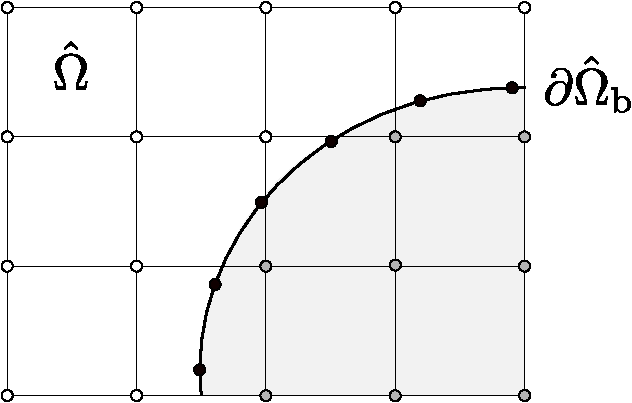
\includegraphics[width=0.32\textwidth]{Images/stressintegration.pdf}
	\caption{Schématické znázornění rozdílu mezi uzly mřížky a body diskretizujícími hranici obtékaného tělesa, které jsou vyznačeny černou barvou.}
	\label{fig:body hranice sim}
\end{figure}


\section{Poznámky k implementaci LBM}\label{poznamky k implementaci LBM}
Jak již bylo zmíněno v úvodu práce, pro numerické řešení pomocí LBM byl využit kód vyvíjený na katedře matematiky (dále jen KM) FJFI ČVUT v Praze, který slouží k řešení Navierových-Stokesových rovnic pro newtonovskou nestlačitelnou tekutinu. Program je implementovaný v jazyce C++ a využívá paralelizace na GPU s využitím platformy CUDA. V kódu je pro model D2Q9 implementována použitá varianta mřížkové Boltzmannovy metody CLBM.

Pro účely této práce byl rozšířen kód vzniklý v rámci předchozí bakalářské práce \cite{JB}, v kterém byla oproti vyvíjenému kódu na KM FJFI  provedena řada úprav, zejména:
\begin{itemize}
	\item implementace metody integrace tenzoru napětí pro výpočet síly pomocí diference,
	\item implementace různých způsobů lokálního výpočtu tenzoru napětí,
	\item implementace interpolačních okrajových podmínek,
	\item výpočet sledovaných veličin a jejich následný výpis do souborů.
\end{itemize}
V kódu byl pak v rámci této práce implementován výpočet zkoumaných účelových funkcí a také momentová okrajová podmínka. Pro implementaci momentové okrajové podmínky pro model D2Q9 byl využit generátor vytvořený Ing. Pavlem Eichlerem implementovaný v C++ využívající knihovnu GiNaC \cite{Ginac}, umožňující provádět symbolické matematické operace.

\chapter{Generování geometrie}\label{geometrie}
V této práci budeme v rámci všech numerických simulací předpokládat rigidní geometrii. To umožní před spuštěním numerické simulace vygenerovat všechny potřebné objekty, které lze během numerické simulace použít. Konkrétně je mimo jiné možné před začátkem numerických výpočtů určit, v jakých bodech diskrétní mřížky se bude nacházet překážka, vypočítat hodnoty parametru $ \Theta $ ze sekce \ref{interpolation bc} a určit tvary normálových vektorů v bodech, které jsou použity pro výpočet síly, jak bylo popsáno v~sekci~\ref{vypocet sily v LBM}.

V této sekci popíšeme použitý proces generování geometrie použitý v rámci této práce. Jelikož k numerickým simulacím využita mřížková Boltzmannovu metoda (viz kapitola \ref{lbm}), je tomu proces generování geometrie uzpůsoben a jeho cílem je připravit data tak, aby pak mohla být vhodně využita v rámci diskrétní ekvidistantní mřížky použité v LBM. 

\section{Struktura generovaných dat}\label{struktura dat}
Výsledná vygenerovaná geometrie je na závěr exportována jako datový soubor, který lze v rámci numerické simulaci načíst. Nejdříve tedy popíšeme strukturu exportovaného souboru. Jak již bylo zmíněno, hlavním cílem generátoru je popsat jednotlivé body mřížky použité v LBM.

U každého bodu mřížky lze jednoznačně určit jeho souřadnice na mřížce a zda se v něm nachází překážka. Dále můžeme v každém bodu určit hodnoty interpolačních parametrů $ \Theta $ pomocí \eqref{eq:q} - pokud se v okolí bodu v daném směru nenachází hranice žádného objektu, definujeme z implementačních důvodů hodnotu přílušného interpolačního parametru jako $ -1$. Výpočet interpolačního parametru bude podrobněji rozebrán později.

V každém z bodů můžeme tedy určit souřadnice $ x $ a $ y $, informaci o přítomnosti překážky a dále celkem 8 různých hodnot interpolačního parametru. Při použití diskrétní mřížky ve tvaru \eqref{eq:oblast} exportovaný soubor tedy obsahuje matici rozměru $ c \times 11$, kde $ c $  označuje kardinalitu množiny $ \hat{\Omega} $ z \eqref{eq:oblast}.

Podotkněme, že pokud je předmětem zkoumání síla působící na obtékaný objekt, je nutné mimo právě popsaný exportovaný soubor předat dále také pole obsahující informaci o normálových vektorech v lagrangeovských bodech, které diskretizují hranici objektu. Výpočet normálových vektorů na hranici je podorobněji popsán dále. Jelikož v této práci není zkoumáno silové působení, uvažujeme pouze export souboru popsaného výše.

\section{Výpočet normálového vektoru}
V případě, kdy je přímo zadán analytický předpis hranice diskretizovaného objektu, lze hodnoty normálového vektoru v každém z bodů diskretizujících hranici jednoduše nalézt pomocí metod matematické analýzy. Pokud nemáme k dispozici analytický popis hranice, můžeme hranici po částech lineárně aproximovat spojením sousedních lagrangeovských bodů úsečkou. Normálové vektory v jednotlivých bodech pak můžeme aproximovat průměrem normálových vektorů ze sousedních bodů. Schematicky je tato konstrukce vyobrazena na obr. \ref{fig:aproximace hranice}.


\begin{figure}[H]
	\centering
	\vspace{2.8mm}
	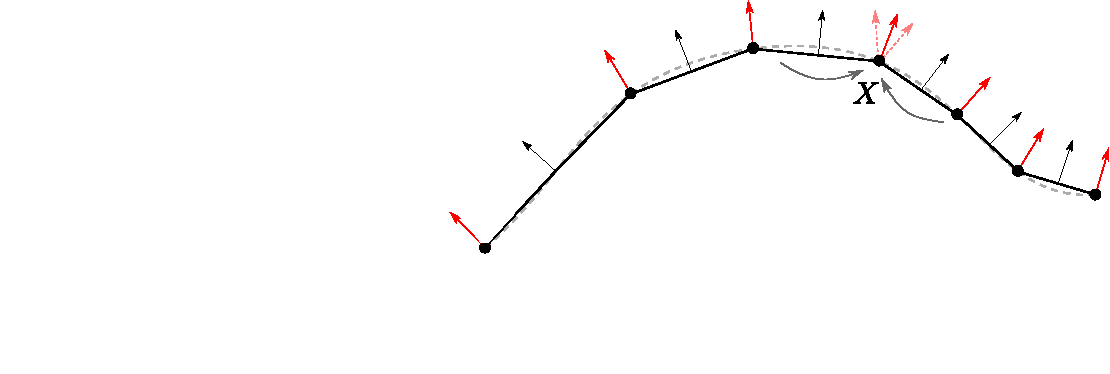
\includegraphics[width=0.7\textwidth, trim={7.9cm 1.6cm 0cm 0cm}]{Images/lincurve.pdf}
	\vspace{1.8mm}
	\caption{Ilustrace konstrukce normálových vektorů u obecné křivky bez zadaného analytického předpisu. $ \boldsymbol{X} $ představuje jeden z lagrangeovských bodů diskretizujících hranici. Tvar hranice, která je po částech lineárně nahrazena, je znázorněn čárkovaně.}
	\label{fig:aproximace hranice}
	\vspace{0mm}
\end{figure}


\section{Výpočet interpolačního parametru}
Pro výpočet interpolačního parametru $ \Theta $ nyní opět předpokládejme, že máme k dispozici analytický popis křivky popisující hranici nebo využijeme již zmíněné po částech lineární aproximace. To jednoznačně určuje vazbu $ \phi = 0$ určující tvar spojité hranice objektu.

Parametr $ \Theta $ je nutné vypočítat pro každý ze směrů možného šíření kromě směru odpovídajícímu $ \vec{\xi}_0 $. V rámci modelu D2Q9 tedy celkem určujeme 8 hodnot pro každý bod hranice, označme je $ \Theta_1, \Theta_2, \dots, \Theta_8$, kde číslo indexu odpovídá příslušnému směru, viz obr. \ref{fig:d2q9}. Použijeme-li značení z obr. \ref{fig:bouz}, tak lze nahlédnout, že průsečík $ \vec{x}_w $ s hranicí nemůže existovat pro každý ze směrů. Jak již bylo zmíněno, z implementačních důvodů pro směry, ve kterých nenajdeme průsečík s hranicí, pokládáme  $ \Theta_i = -1$, přičemž Bouzidiho interpolační podmínka popsaná v sekci \ref{interpolation bc} v těchto směrech není použita.

Interpolační parametr získáme vypočtením průsečíku hranice a úsečky ve směru $ \vec{\xi}_i $. Opět s použitím značení z obr. \ref{fig:bouz} parametrizujme úsečku spojující body $ \vec{x}_{f{_A}} = (x_{f{_A}}, y_{f{_A}})$ a $ \vec{x}_b  = (x_b, y_b)$ jako
\begin{align}\label{eq:parametrizace usecky}
\begin{split}
x=& s \, x_{f{_A}} + (1 - s) \, x_b,
\\
y=& s \, y_{f{_A}} + (1 - s) \, y_b ,
\end{split}
\end{align}
kde $ s \in \langle 0, 1 \rangle $. Dále dosazením \eqref{eq:parametrizace usecky} do rovnice vazby $ \phi $ získáme obecně nelineární rovnici pro $ s $. Tuto rovnici řešíme v rámci generátoru pomocí Powellovy hybridní metody \cite{Powell}, která je dostupná v rámci knihovny SciPy implementované v jazyce Python. Je snadné nahlédnout, že získaná hodnota $ s $ pak odpovídá hledané hodnotě parametru $ \Theta_i $, a není tedy nutné explicitně počítat souřadnice bodu  $ \vec{x}_w $ a používat vztah \eqref{eq:q}. Podotkněme, že v rámci tohoto kroku předpokládáme, že řešení výše zmíněné nelineární rovnice bude nejvýše jedno, což však nepředstavuje výrazné omezení pro tvary objektů, které můžeme použít.

\section{Struktura kódu a poznámky k implementaci}\label{meshgenenator}
Generátor 2D geometrie použitý v rámci této práce byl objektově implementovaný v programovacím jazyce Python s využitím volně dostupných knihoven. Celý generátor tvoří samostatný balík jménem \texttt{meshgenerator}. V této sekci krátce popíšeme strukturu a fungování tohoto balíku sestávajícího ze tří hlavních částí. Struktura a propojení tříd v rámci balíku \texttt{meshgenerator} je znázorněna na obr. \ref{fig:uml meshgenerator}.

První část obsahuje pomocné funkce a pomocnou třídu \texttt{Point}, která rezprezentuje jeden bod na mřížce, tedy mezi její atributy patří souřadnice, informace o přítomnosti překážky a hodnoty interpolačních parametrů.

Druhá část se skládá z jednotlivých modulů, které obsahují třídy a podtřídy reprezentující jednotlivé objekty, které lze v rámci simulace použít. Potomkem rodičovské třídy \texttt{GeneralObject}, která zastřešuje veškeré použitelné objekty, je třída \texttt{ClosedObject}, resp. \texttt{OpenObject},  reprezentující objekty s definovaným vnitřkem, resp. objekty bez jednoznačně definovaného vnitřku. Třída \texttt{OpenObject} tedy navíc obsahuje atribut nesoucí informaci o orientaci objektu v oblasti, díky němuž lze pak jednoznačně objekt vymezit. Ze třídy \texttt{ClosedObject} jsou pak dále odvozené třídy \texttt{Polygon} (reprezentuje objekty ve tvaru mnohoúhelníka) a \texttt{Implicit} (reprezentuje objekty, které jsou definovány pomocí implicitního vztahu). Pro následné zjednodušení práce s konkrétními implicitně zadanými objekty byly definovány třídy \texttt{Circle} (reprezentuje objekty ve tvaru kružnice), \texttt{Ellipse} (reprezentuje objekty ve tvaru elipsy) a \texttt{CassiniOval} (reprezentuje objekty ve tvaru Cassiniho oválu\footnote{Cassiniho ovál je křivka pojmenovaná po Giovannim Cassinim. Jsou-li $ P_1 $ a $ P_2 $ dva pevné body v rovině a $ b > 0$, pak je Cassiniho ovál formálně definován jako množina $$ \left\{ \, P \: \big| \: |PP_1|\cdot|PP_2| = b^2 \, \right\} ,$$ tedy množinou bodů, jejichž součin vzdáleností od $ P_1 $ a $ P_2 $ je konstantní.}) Ze třídy \texttt{OpenObject} jsou odvozené třídy \texttt{FunctionCurve} (reprezentuje objekty zadané pomocí explicitního funkčního předpisu) a \texttt{SVGCurve} (reprezentuje křivku, která byla vytvořena ve formátu $\mathtt{SVG} $ \cite{Eisenberg2002}). Pro případné jednodušší generování zúžených cév pak byla implementována třída \texttt{Exponential}, která je potomkem třídy \texttt{FunctionCurve}. Model stenózy cévy vzniklý použitím instancí třídy \texttt{Exponential} je prezentován na obr. \ref{fig:vessel exponential}. Podotkněme, že všechny implementované objekty byly vybrány tak, aby byly lehce popsatelné pomocí několika parametrů a byly tak vhodné pro využití v rámci optimalizace, která je předmětem této práce. Výjimku tvoří třída \texttt{SVGCurve}, která vznikla v rámci předchozí bakalářské práce a která nevyužívá k vytvoření objektu žádného parametru a nelze ji tak v rámci optimalizace použít.


\begin{figure}[h]
	\centering
	\vspace{8mm}
	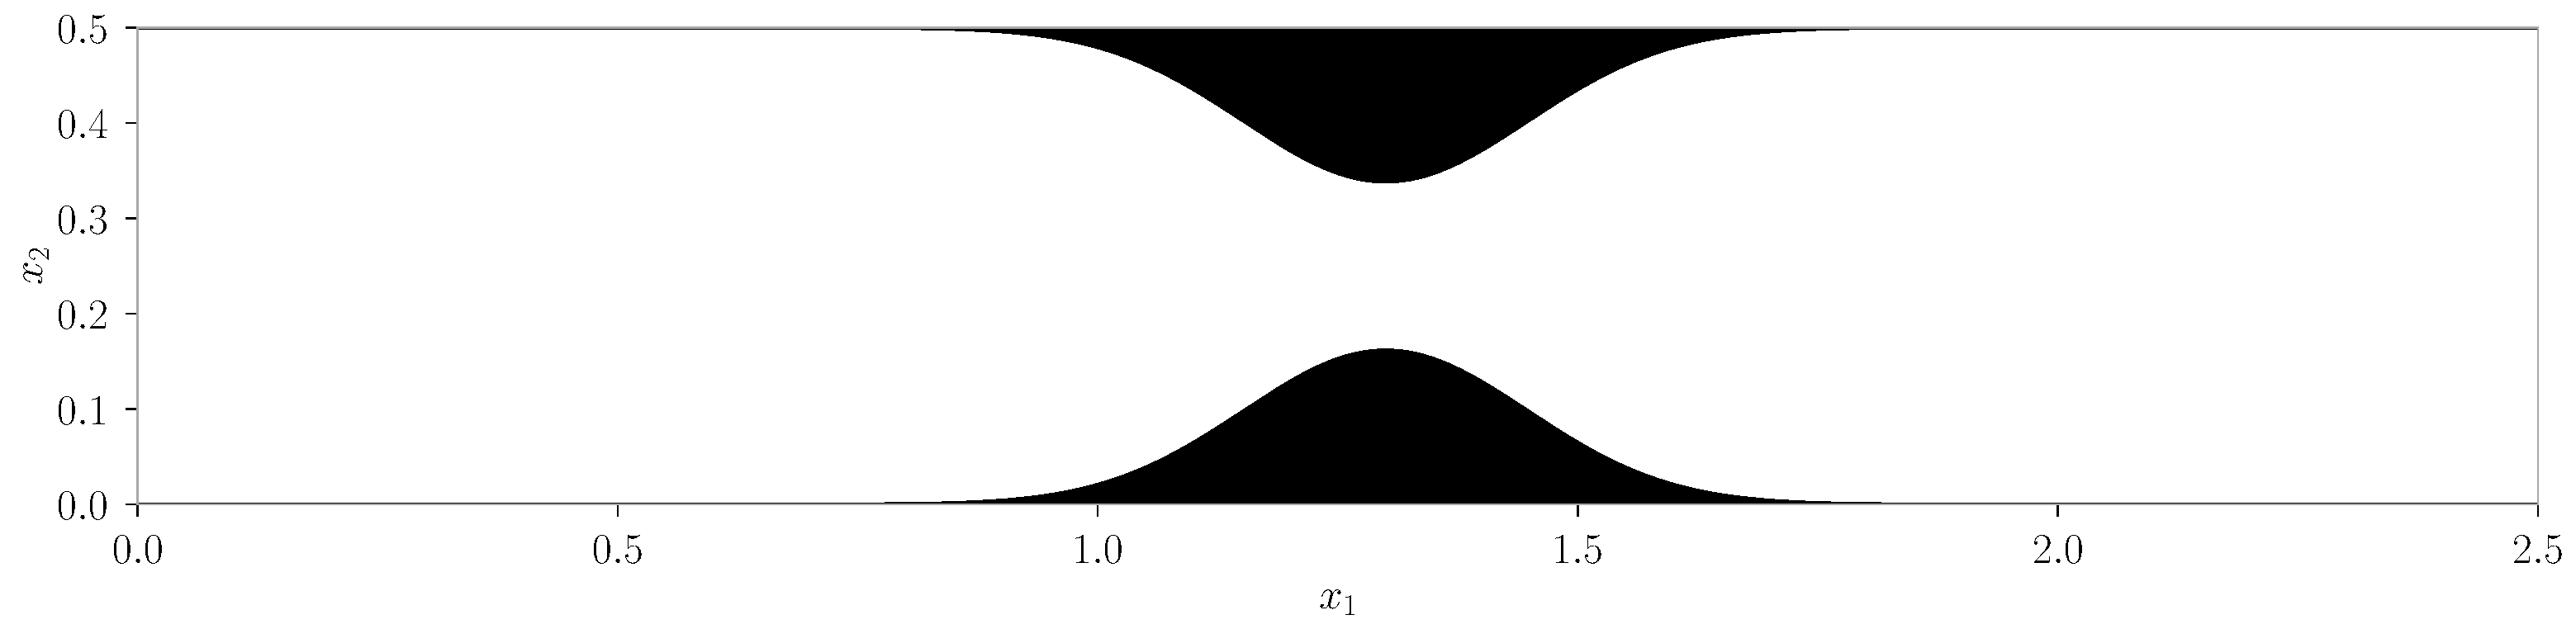
\includegraphics[width=0.95	\textwidth]{Images/figvessel.pdf}
	\vspace{2mm}
	\caption{Model stenózy cévy vzniklý použitím instancí třídy \texttt{Exponential}.}
	
	\label{fig:vessel exponential}
	\vspace{1.8mm}
\end{figure}

Třetí část balíku \texttt{meshgenerator} pak definuje třídu \texttt{NumSimProblem}, která souhrnně definuje celou úlohu, jež je dále numericky řešena. Pomocí konfiguračního souboru, v kterém jsou definovány uživatelem požadované parametry výpočetní oblasti, je inicializována datová struktura popsaná v sekci \ref{struktura dat} obsahující veškeré body diskrétní mřížky použité v LBM. Konstruktoru třídy \texttt{NumSimProblem} jsou dále předány všechny instance podtříd třídy \texttt{GeneralObject}, které tvoří celkovou požadovanou geometrii a které jsou dále využity pro aktualizaci informací o jednotlivých bodech mřížky. Vygenerovaná datová struktura je pak exportována a dále využita v rámci numerické simulace.

\begin{figure}[h]
	\centering
	\vspace{8mm}
	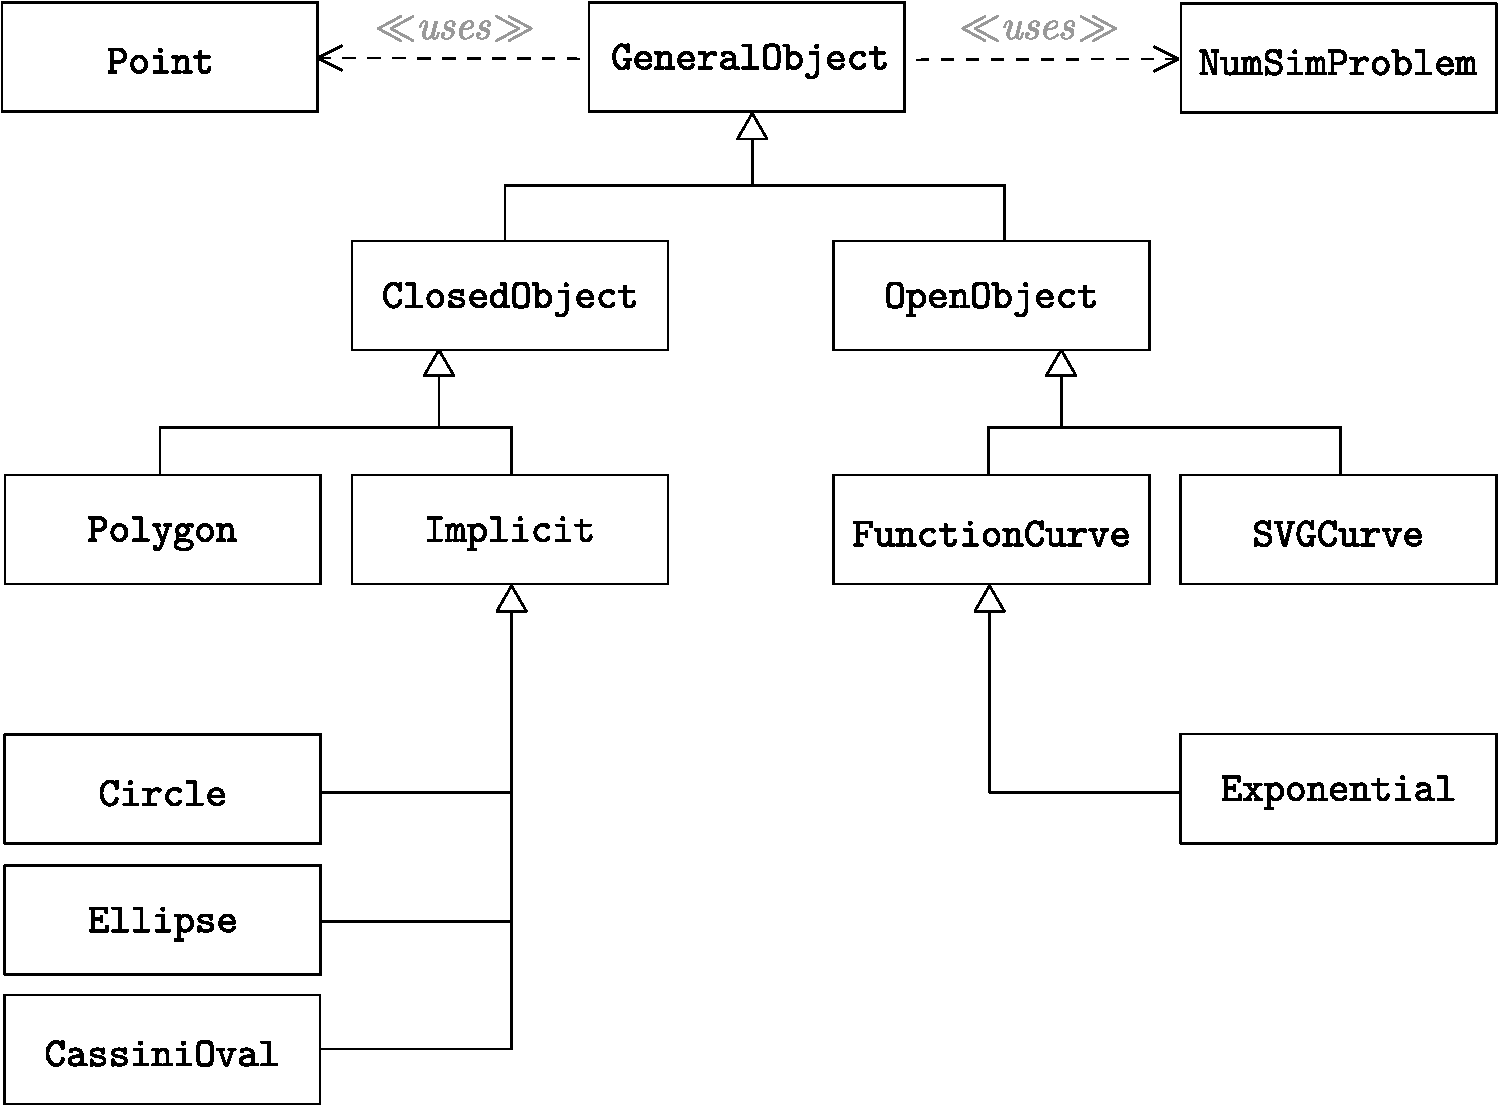
\includegraphics[width=0.9	\textwidth]{Images/umldiagram.pdf}
	\vspace{2mm}
	\caption{Diagram znázorňující strukturu a využití tříd v rámci balíku \texttt{meshgenerator}.}
	\label{fig:uml meshgenerator}
	\vspace{1.8mm}
\end{figure}
\chapter{Matematická optimalizace}\label{optimalizace}

Matematická optimalizace (jinak také matematické programování) je rozsáhlý obor zahrnující řadu disciplín, mezi které patří např. lineární a nelineární optimalizace, konvexní programování, celočíselné programování a jiné \cite{Bert}. Cílem této kapitoly je shrnout základní koncepty a techniky relevantní pro tuto práci. Nejprve představíme základní úlohu zkoumanou v rámci optimalizace, dále popíšeme některé z technik řešení úloh bez vazeb a s vazbami. Poté rozebereme optimalizaci úloh, v nichž obecně není známý předpis účelové funkce. Na závěr popíšeme celkový optimalizační rámec aplikovaný na optimalizaci úloh v této práci.

\section{Základní optimalizační úloha}

Buďte $ m, n, q \in \mathbb{N}$. Dále nechť jsou definovány spojité funkce $ f: \mathbf{D} \rightarrow \mathbb{R}$, $ \vec{g} : \mathbf{D} \rightarrow \mathbb{R}^m $, $ \vec{h} : \mathbf{D} \rightarrow \mathbb{R}^q $, kde $ \mathbf{D} = \mathrm{Dom} \, (f) \cap \mathrm{Dom} \, (g) \cap \mathrm{Dom} \, (h)$, tj. $ \mathbf{D} $ je průnik definičních oborů daných funkcí. Definujme množinu

\begin{equation}\label{eq:pripustna reseni}
\mathbf{X} = \big\{ \vec{x} \in \mathbf{D} \subseteq \mathbb{R}^n \ | \ \vec{g} (\vec{x}) \leq \vec{0} \wedge \vec{h} (\vec{x}) = \vec{0} \, \big\},
\end{equation}
kde nerovnost $ \vec{g} \leq \vec{0} $ a rovnost $ \vec{h} = \vec{0} $  jsou chápány po složkách. Obecně je pak cílem matematické optimalizace řešit úlohu

\begin{equation}\label{eq:zakladni uloha}
	\min_{\vec{x} \in \mathbf{X}} f(\vec{x}).
\end{equation}
Minimalizovanou funkci $ f $ nazýváme účelová funkce, množinu $ \mathbf{D} $ nazýváme definiční obor úlohy, $ \mathbf{X} $~se nazývá množina přípustných řešení \cite{Bert}. Upozorněme, že dále $ f $ bude značit pouze účelovou funkci, nikoliv distribuční funkce z kapitoly \ref{lbm}.

Při klasifikaci optimalizačních problémů hovoříme o tzv. vazbách. Ty jsou určeny definicí množiny~$ \mathbf{X} $, tj. rovnostními a nerovnostními podmínkami pro funkce $ \vec{g} $ a $ \vec{h} $, a tvarem množiny $ \mathbf{D} $. V případě podmínek definovaných $ \vec{g} (\vec{x}) \leq \vec{0} \wedge \vec{h} (\vec{x}) = \vec{0} $ hovoříme o explicitních vazbách, omezení definovaná definičním oborem úlohy $ \mathbf{D} $ nazýváme implicitní.

Prvek $ \vec{x}^{\star} \in  \mathbf{X} $ budeme nazývat optimálním řešením úlohy \eqref{eq:zakladni uloha} za předpokladu, že
\begin{equation}
	\vec{x}^{\star} = \operatorname*{argmin}_{\vec{x} \in \mathbf{X}} \, f(\vec{x}).
\end{equation}
Podotkněme, že optimální řešení nemusí být dáno jednoznačně a množinu všech optimálních řešení úlohy nazveme optimální množina. Je důležité zmínit, že hledání optimálního řešení lze ekvivalentně formulovat také jako hledání maxima z funkce $ -f $ přes stejnou množinu $ \mathbf{X}$, což umožnuje řešit problémy maximalizace pomocí stejných technik, které budou představeny dále \cite{Bert, non-linear-textbook}.

\section{Řešení úlohy bez vazeb}\label{unconstrained}

V této sekci rozebere řešení úlohy bez vazeb, tj. v úloze \eqref{eq:zakladni uloha} budeme předpokládat 
$ \mathbf{X} = \mathbb{R}^n $. Popíšeme pouze část metod, které lze pro řešení optimalizačních úloh bez vazeb použít. Konkrétně se zaměříme na tzv. kvazinewtonovské metody. Detailní popis metod pro řešení úloh bez vazeb lze najít např. v \cite{non-linear-textbook}.

Kvazinewtonovské metody jsou třídou gradientních metod. Mezi gradientní metody dále patří např.~metoda největšího spádu nebo metoda konjugovaných gradientů. Dále popsané algoritmy slouží k~nalezení~stacionárního bodu účelové funkce $ f $, tedy bodu $ \tilde{x} $ takového, že $ \nabla f(\tilde{x}) = 0 $. Za dodatečného předpokladu splnění vhodných podmínek lze pak usoudit, zda se jedná o hledaný globální extrém účelové funkce~\cite{Bert, non-linear-textbook}.

Kvazinewtonovské metody jsou iterativní a jejich hlavní myšlenkou je, že v každé iteraci používají k~určení směru spádu zlepšující se aproximace inverze Hessovy matice $ (\nabla ^2 f(\vec{x}))^{-1} $ založeném na algoritmu pro výpočet inverzní matice. K této aproximaci je v každé iteraci potřeba znalost gradientu účelové funkce. Výpočetní složitost kvazinewtonovských metod je obecně $ O(n^2) $, což poskytuje vylepšení ve srovnání s Newtonovou metodou, jejíž výpočetní složitost je $ O(n^3) $ \cite{non-linear-textbook}. Dále se zaměříme na dva konkrétní používané kvazinewtonovské algoritmy.

\subsection{Davidonův-Fletcherův-Powellův algoritmus}\label{DFP}
První představenou kvazinewtonovskou metodou je Davidonův-Fletcherův-Powellův (dále jen DFP) algoritmus \cite{Fletcher1963}. Dále budeme značit $ H_k $ aproximaci inverze Hessovy matice v $ k $-té iteraci, na začátku incializujeme $ H_0 = I $. Algoritmus DFP lze pak shrnout v následujících krocích:

\begin{enumerate}
	\item \textbf{Inicializace:} Volba $ \vec{x}_0 \in \mathbf{X}$ a následné vypočtení $ \vec{g}_0 = \nabla f (\vec{x}_0) $. Nastavení hodnot $ k=0 $ a $ H_0 = I $.
	\item \textbf{Cyklus} končící splněním podmínky ukončení, která je zadána uživatelem. Z důvodu konečné strojové přesnosti typicky požadujeme, aby vypočtená hodnota gradientu byla menší než požadovaný parametr $ \varepsilon > 0$.
	\begin{enumerate}
		\item \textbf{Vypočtení směru hledání} jako $ \vec{d}_k = -H_k \vec{g}_k $.
		\item \textbf{Jednorozměrná minimalizace}, při které najdeme $ \alpha_k = \operatorname*{argmin}_{\alpha \geq 0} f (\vec{x}_k + \alpha \vec{d}_k)$.
		\item \textbf{Vypočtení a nastavení hodnot:}
		\begin{subequations}
			\begin{eqnarray}
			\vec{x}_{k+1} &=& \vec{x}_k + \alpha_k \vec{d}_k,\\[3pt]
			\vec{g}_{k+1} &=& \nabla f({\vec{x}_{k+1}}).
			\end{eqnarray}
		\end{subequations}
		\item \textbf{Aproximace inverze Hessovy matice:} 
		\begin{subequations}
			\begin{eqnarray}
			\vec{p}_{k} &=& \vec{x}_{k+1} - \vec{x}_{k},\\[3pt]
			\vec{q}_{k} &=& \vec{g}_{k+1} - \vec{g}_{k},\\[3pt]\label{eq:hessian}
			H_{k+1} &=& H_k - \frac{1}{\vec{q}^T_k H_k \vec{q}^{}_k} (H_k \vec{q}^{}_k)(H_k \vec{q}^{}_k)^T + \frac{1}{\vec{p}^T_k \vec{q}^{}_k} (\vec{p}^{}_k \vec{p}^{T}_k).
			\end{eqnarray}
		\end{subequations}
		\item \textbf{Nastavení} $ k = k + 1 $.
	\end{enumerate}
	\item \textbf{Konec algoritmu.}
\end{enumerate}
Posloupnost vektorů $ \vec{x}_k $ v algoritmu konverguje k řešení úlohy. Jedním z teoretických výsledků týkajích se DFP algoritmu je fakt, že pro $ f $ konvexní konverguje ke stacionárnímu bodu pro libovolnou volbu počátečního vektoru $ \vec{x}_0 $ \cite{non-linear-textbook}.

\subsection{Broydenův-Fletcherův-Goldfarbův-Shannoův algoritmus}\label{BFGS}
Druhou kvazinewtonovskou metodou, kterou popíšeme, je Broydenův-Fletcherův-Goldfarbův-Shannoův (dále jen BFGS) algoritmus \cite{broyden1970}. BFGS algoritmus je modifikací DFP algoritmu, s kterým sdílí všechny jeho kroky, jedinou jeho odlišností je využití jiné aproximace inverze Hessovy matice. BFGS algoritmus nahrazuje rovnici \eqref{eq:hessian} vztahem
\begin{equation}
	H_{k+1} = H_k - \frac{1}{\vec{p}^{T}_{k} \vec{q}^{}_k} \left[ \vec{p}^{}_{k} (H_k \vec{q}^{}_k)^T + (H_k \vec{q}^{}_k) \vec{p}^T_k - \left( 1 + \frac{\vec{q}^T_k H_k \vec{q}^{}_k}{\vec{p}^T_k \vec{q}^{}_k} \right) (\vec{p}^{}_k \vec{p}^{T}_k) \right].
\end{equation}
Z hlediska konvergence se dá BFGS algoritmus považovat za lepší než DFP. Za zmínění stojí modifikace BFGS algoritmu jménem L-BFGS (nebo LM-BFGS, z anglického \textit{limited-memory BFGS}), která pracuje pouze s omezeným množstvím počítačové paměti, a proto je její využití vhodné pro úlohy s vyšší dimenzí~\cite{Byrd1995}.

\section{Řešení úlohy s vazbami}\label{constrained}
Budeme nyní uvažovat úlohu \ref{eq:zakladni uloha} z úvodu kapitoly, kde množina přípustných řešení má tvar \ref{eq:pripustna reseni}. V~této sekci popíšeme, jak tuto úlohu řešit převedením na posloupnost optimalizačních úloh bez vazeb, jejichž řešení bylo diskutováno v sekci \ref{unconstrained}. Opět existuje více způsobů, jak úlohy s vazbami řešit, zde však popíšeme pouze řešení pomocí penalizačních a bariérových metod.

\subsection{Penalizační metody}\label{penalty method}
Jak již bylo řečeno, penalizační metody převádí řešení omezených úloh na úlohy bez omezení. Základním principem penalizačních metod je zohlednění podmínek vymezujících množinu přípustných řešení tak, že k účelové funkci přidáme penalizační člen, který reflektuje míru překročení daných podmínek \cite{Bert}. Jako penalizační funkci budeme označovat spojitou skalární funkci na $ \mathbb{R}^n $ splňující

\begin{align}
\begin{split}
p(\vec{x}) &=0, \ \ \forall \vec{x} \in \mathbf{X},\\[6pt]
p(\vec{x}) &>0, \ \ \text { jinak. }
\end{split}
\end{align}
Typickou volbou penalizační funkce je např.
\begin{equation}\label{eq:penalty function}
p (\vec{x}) = \sum_{j=1}^{m} \left( \, \max  \left\{ \,  g_j (\vec{x}), 0 \,  \right\} \, \right)^2 + \sum_{j=1}^{q} h_j (\vec{x})^2.
\end{equation}


Pomocí penalizační funkce $ p $ dále sestrojíme modifikovanou účelovou funkci 
\begin{equation}\label{eq:cost function with penalty}
	\phi (\vec{x}, r) = f (\vec{x}) + r p(\vec{x}),
\end{equation}
kde $ r > 0 $ nazýváme penalizační parametr \cite{Bert}. Z definice penalizační funkce můžeme vidět, že hodnoty modifikované účelové funkce $ \phi (\vec{x}, r)$ jsou různé od původní funkce $ f $ pouze pro taková $ \vec{x} $, kdy je porušena zadaná zohledněná podmínka.

Pro řešení úlohy s vazbami budeme v každé iteraci konstruovat nový člen ostře rostoucí posloupnosti penalizačních parametrů $ r_1, r_2, \dots$, pro který budeme řešit optimalizační úlohu bez vazeb pro modifikovanou funkci $ \phi (\vec{x}, r_k)$. Optimální řešení $ \vec{x}_k $ této úlohy bez vazeb (nalezené např. technikami popsanými v sekci \ref{unconstrained}) využijeme jako počáteční bod pro další iteraci. Toto opakujeme dokud není splněna podmínka $ r_k p(\vec{x}_k) < \varepsilon$ pro zvolené $  \varepsilon > 0$, při splnění této podmínky lze $ \vec{x}_k $ považovat za postačující aproximaci řešené úlohy s vazbami. Podotkněme, že penalizační metody umožňují hledat optimální řešení během jednotlivých iterací mimo množinu přípustných řešení \cite{non-linear-textbook}, proto jsou řazeny mezi tzv. metody vnějšího bodu. Důležitým předpokladem penalizačních metod je, aby definiční obor úlohy splňoval $ \mathbf{D} = \mathbb{R}^n $.

Konstrukce posloupnosti penalizačních parametrů a princip penalizační metody je znázorněn na obr.~\ref{fig:penalty} na triviálním příkladu minimalizace funkce $ f(x) = 0,5x $ s podmínkou $ g(x) = 4 - x \leq 0 $. Modifikovaná účelová funkce má v tomto případě tvar 
\begin{equation}
	 \phi (x, r) = 0,5x + r \left(\max  \left\{ \,  4-x, 0 \right\}\right)^2.
\end{equation}

\begin{figure}[H]
	\centering
	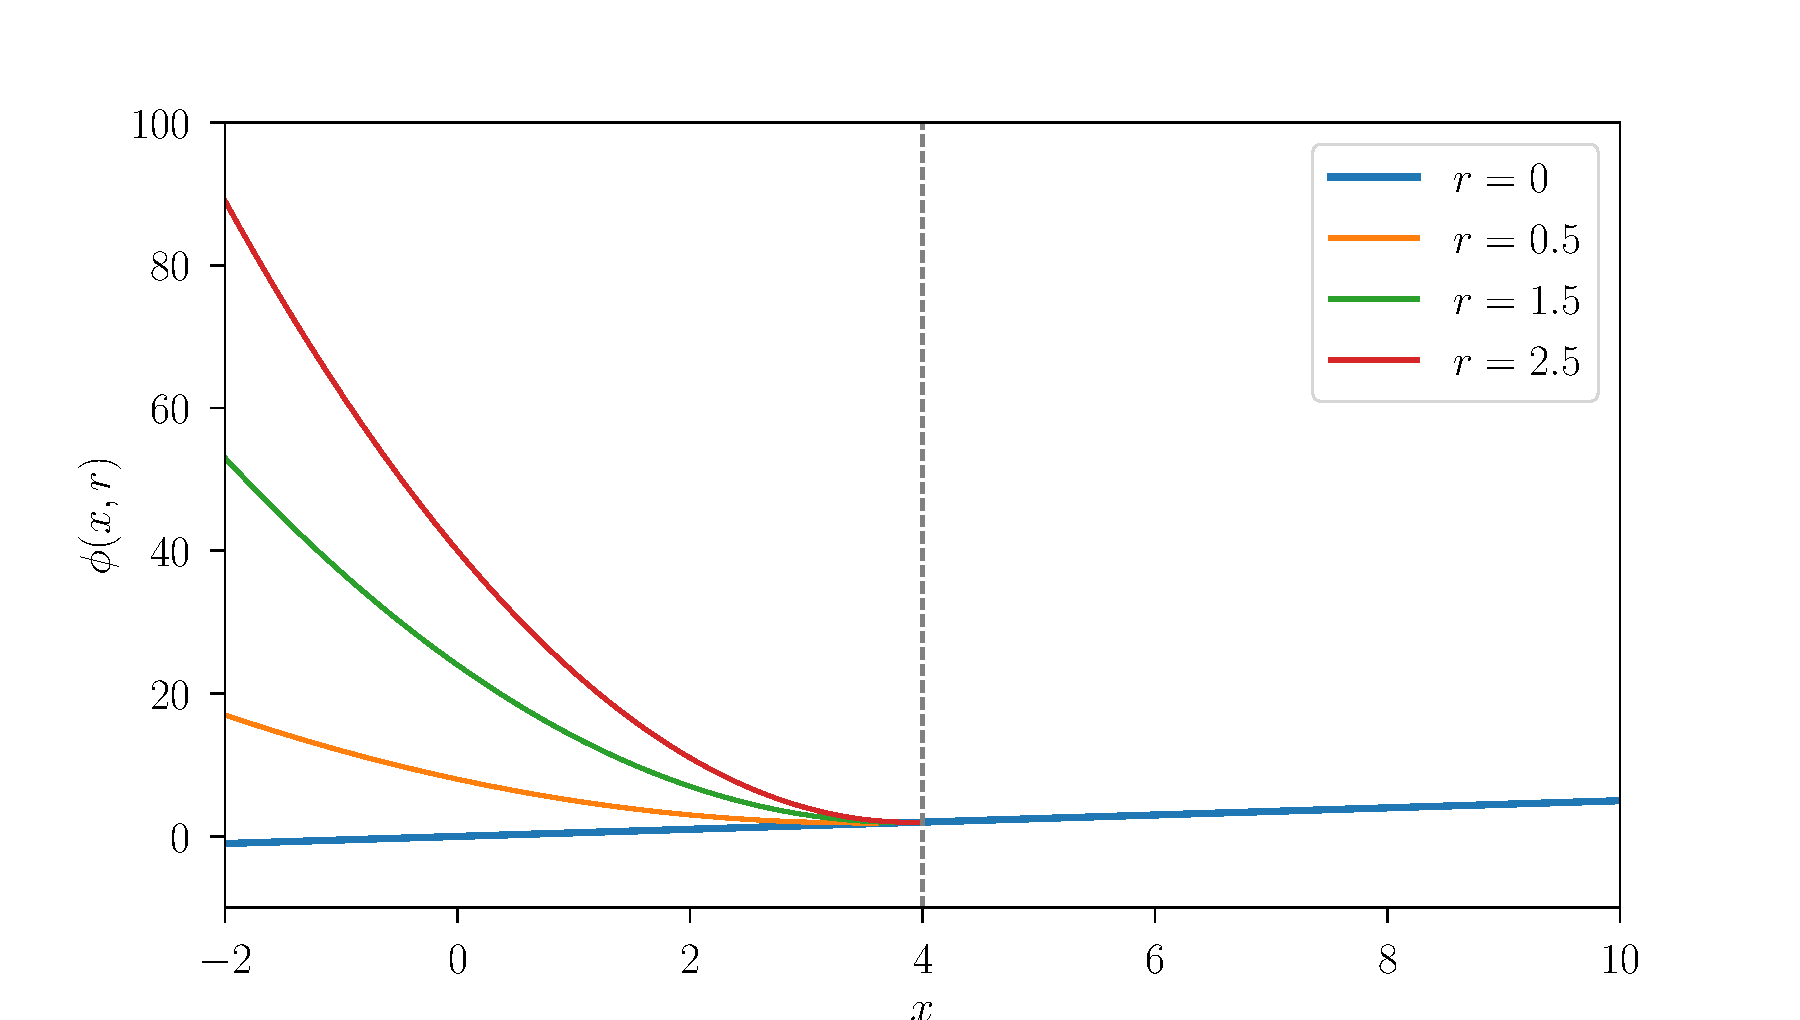
\includegraphics[width=1.0\textwidth]{Images/penalty.pdf}
	\vspace{0.25cm}
	\caption{Ilustrace penalizační metody použité pro minimalizaci funkce $ f(x) = 0,5x $ s podmínkou $ g(x) = 4 - x \leq 0 $. Barevně jsou odlišeny různé tvary modifikované účelové funkce $\phi (x, r)  $ v závislosti na hodnotě penalizačního parametru $ r $. Podmínka vymezující množinu přípustných řešení je vyznačena šedě čárkovaně. Množina přípustných řešení se nachází v polorovině napravo od této šedé čárkované osy.}
	\label{fig:penalty}
\end{figure}

\subsection{Bariérová metoda}\label{barrier method}
Bariérová metoda využívá podobného principu jako penalizační metody, jejím hlavním rozdílem však je, že při iterativním hledání optimálního řešení úlohy s vazbami je garantováno, že odhady řešení vždy budou prvky vnitřku přípustné množiny, který má tvar
\begin{equation}
\mathbf{X}^{\mathrm{o}} = \big\{ \vec{x} \in \mathbf{D} \subseteq \mathbb{R}^n \ | \ \vec{g} (\vec{x}) < \vec{0} \, \big\}.
\end{equation}
Metody splňující tuto podmínku se obecně nazývají metody vnitřního bodu \cite{non-linear-textbook}.

Opět zohledníme podmínky vymezující množinu přípustných řešení tak, že k účelové funkci přidáme nový člen, který reflektuje míru jejich překročení. Jako bariérovou funkci $ B $ budeme chápat spojitou skalární funkci na $ \mathbf{X}^{\mathrm{o}} $ splňující podmínku
\begin{equation}
	(\exists j \in \{1,2,\dots,m\})(\lim\limits_{\substack{\vec{x} \to \vec{y} \\ \mathbf{X}^{\mathrm{o}}}} g_j (\vec{x}) = 0) \Rightarrow \lim\limits_{\substack{\vec{x} \to \vec{y} \\ \mathbf{X}^{\mathrm{o}}}} B (\vec{x}) = + \infty.
\end{equation}
Typickou volbou bariérové funkce je např. logaritmická bariérová funkce
\begin{equation}\label{eq:log barrier function}
B (\vec{x}) = -\sum_{j=1}^{m} \ln \left( \, - g_j (\vec{x}) \right),
\end{equation}
nebo dále např. reciproká bariérová funkce
\begin{equation}\label{eq:reciprocal barrier function}
B (\vec{x}) = -\sum_{j=1}^{m} \frac{1}{g_j (\vec{x})}.
\end{equation}
Pomocí barierové funkce $ B $, podobně jako u penalizačních metod, sestrojíme modifikovanou účelovou funkci 
\begin{equation}\label{eq:cost function with barrier}
\phi (\vec{x}, r) = f (\vec{x}) + r B(\vec{x}),
\end{equation}
kde $ r > 0 $ je volený parametr \cite{non-linear-textbook}.

Pro řešení úlohy s vazbami pomocí bariérové metody budeme v každé iteraci konstruovat nový člen kladné ostře klesající posloupnosti parametrů $ r_1, r_2, \dots$, pro který budeme řešit optimalizační úlohu bez vazeb pro modifikovanou funkci $ \phi (\vec{x}, r_k)$. Vektor $ \vec{x}_k  = \operatorname*{argmin}_{\vec{x} \in \mathbf{X}^\mathrm{o}} (f (\vec{x}) + r_k B(\vec{x}))$ určený optimalizací úlohy bez vazeb využijeme jako počáteční bod pro další iteraci. Toto opakujeme dokud není splněna podmínka $ r_k < \varepsilon$ pro zvolené $  \varepsilon > 0$, při splnění této podmínky $ \vec{x}_k $ považujeme za postačující aproximaci řešené úlohy s vazbami \cite{non-linear-textbook}.

Dále zmíníme volbu bariérové funkce $ B_{\infty} $ využívané k definici tzv. extrémní bariérové funkce (anglicky \textit{extreme barrier function}), jak se nazývá modifikovaná účelová funkce při této volbě \cite{BBO-textbook}. Tato bariérová funkce kopíruje asymptotické chování výše zmíněných bariérových funkcí a má tvar
\begin{align}
\begin{split}
B_{\infty}(\vec{x}) &=0, \ \ \forall \vec{x} \in \mathbf{X},\\[6pt]
B_{\infty}(\vec{x}) &=+\infty, \ \ \text { jinak. }
\end{split}
\end{align}
Modifikovaná účelová funkce (extrémní bariérová funkce) má pak tvar
\begin{align}\label{eq:extreme barrier}
\begin{split}
f_{\infty}(\vec{x}) &=f(\vec{x}) , \ \ \forall \vec{x} \in \mathbf{X},\\[6pt]
f_{\infty}(\vec{x}) &=+\infty, \ \ \text { jinak. }
\end{split}
\end{align}

Konstrukce posloupnosti parametrů $ (r_k)_{k \in \mathbb{N}} $ a princip bariérové metody je znázorněn na obr.~\ref{fig:barrier} opět na příkladu minimalizace funkce $ f(x) = 0,5x $ s podmínkou $ g(x) = 4 - x \leq 0 $ a volbou reciproké bariérové funkce. Modifikovaná účelová funkce má tvar 
\begin{equation}
\phi (x, r) = 0,5x - \frac{r}{4-x}.
\end{equation}

\begin{figure}[H]
	\centering
	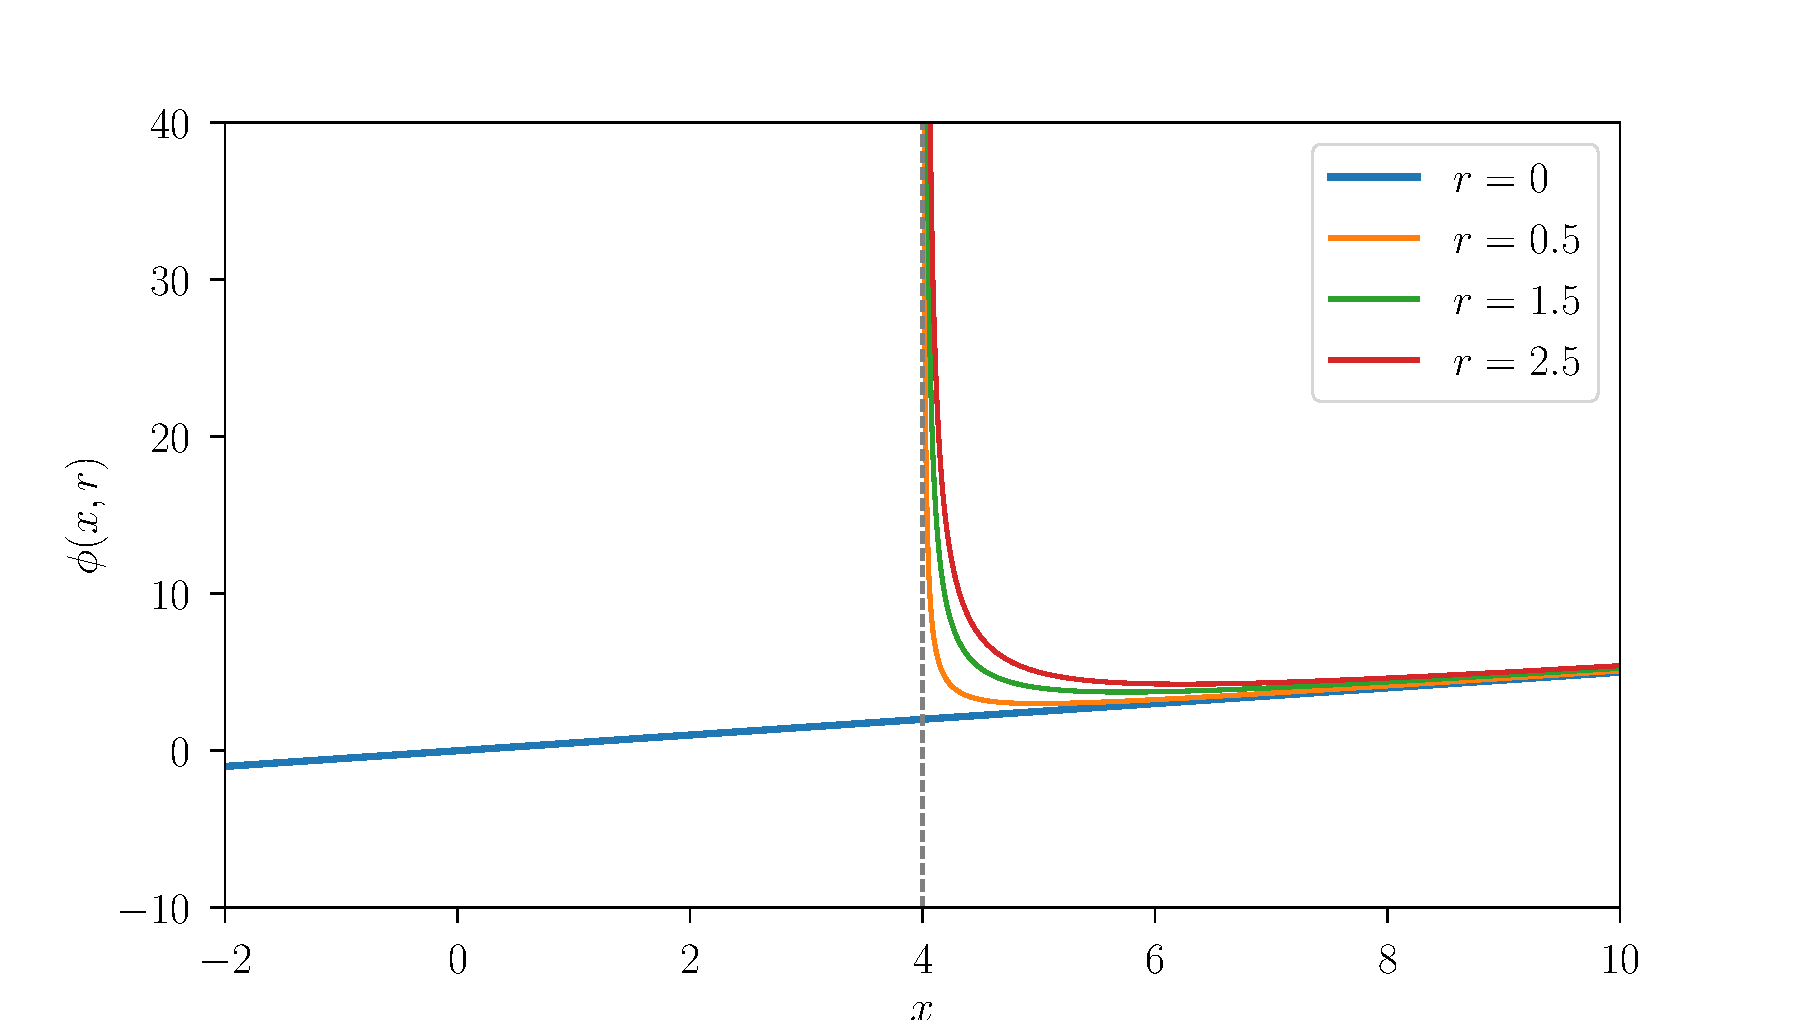
\includegraphics[width=1.0\textwidth]{Images/barrier.pdf}
	\caption{Ilustrace bariérové metody použité pro minimalizaci funkce $ f(x) = 0,5x $ s podmínkou $ g(x) = 4 - x \leq 0 $. Barevně jsou odlišeny různé tvary modifikované účelové funkce $\phi (x, r)  $ v závislosti na hodnotě penalizačního parametru $ r $. Podmínka vymezující množinu přípustných řešení je vyznačena šedě čárkovaně. Množina přípustných řešení se nachází v polorovině napravo od této šedé čárkované osy.}
	\label{fig:barrier}
\end{figure}

\section{Black-box optimalizace}\label{black-box}
V praxi je běžné setkat se s případy, kdy je nutné v rámci řešení úlohy optimalizovat účelovou funkci~$ f $, jejíž analytický předpis stejně jako předpis pro výpočet derivace není známý. Tento problém je typický např. pro výsledky numerických simulací, kdy účelovou funkci dokážeme pouze vyčíslit v konkrétním bodě a získat tak požadovanou funkční hodnotu. Často pak v praxi také samotné vyčíslení funkce v bodě může představovat problém a může být např. velmi časově nebo výpočetně náročné. Zjevně pro řešení problémů tohoto charakteru není vhodné použít výše zmíněné standardní optimalizační algoritmy.

Řešením úloh, v kterých je účelová funkce (popř. i zadané vazby) dána pomocí tzv. black-boxu\footnote{Jako black-box se v programování označuje systém, jehož vnitřní mechanismy nejsou uživateli známy. To znamená, že uživateli je přístupný obecně pouze vstup a výstup daného systému \cite{BBO-textbook}.}, se zabývá disciplína jménem black-box optimalizace (dále jen BBO). V rámci BBO typicky není předpokládáno, že by účelová funkce byla spojitá nebo diferencovatelná \cite{BBO-textbook, derivative-free-review, two-decades}.

Podotkněme, že v literatuře se často black-box optimalizace zaměňuje s bezgradientní optimalizací (anglicky \textit{derivative-free optimization}, dále jen DFO), která zahrnuje metody a techniky pro účelové funkce, jejichž derivace není známa či je obtížné ji vypočítat \cite{BBO-textbook, derivative-free-review, Kramer2011}. Tyto dvě disciplíny sdílí řadu společných vlastností, liší se však zejména v tom, že v rámci DFO může být předpis pro výpočet derivace účelové funkce známý. Dále BBO v sobě zarhnuje i heuristické metody, zatímco DFO se zaměřuje zejména na metody, které mohou být spolehlivě matematicky analyzovány z hlediska konvergence a stanovení zastavovací podmínky, což pro metody BBO mnohdy není možné \cite{BBO-textbook}. Proto ačkoliv, jak bylo zmíněno, se pojmy BBO a DFO často zaměňují, v rámci této práce je budeme chápat jako dvě rozdílné disciplíny \cite{BBO-textbook}.

Dále podotkněme, že v literatuře lze najít různé klasifikace metod v rámci BBO. V rámci této práce se budeme držet klasifikace uvedené v \cite{BBO-textbook} a budeme tedy odlišovat heuristické metody, metody přímého vyhledávání a metody založené na využití náhradního modelu. Každou z těchto tříd v této sekci krátce popíšeme.

\subsection{Heuristické metody}\label{heuristic}
Mezi heuristické optimalizační metody patří mimo jiné třída genetických algoritmů, která je blíže popsána v \cite{BBO-textbook} společně s dalšími různými heuristickými metodami. V této sekci popíšeme jinou používanou heuristickou metodu, a to Nelderovu-Meadovu metodu (v textu dále někdy označována zkratkou NM), také někdy označovanou jako simplexová\footnote{Simplexem v $ \mathbb{R}^n $ nazýváme omezený konvexní polytop (zobecnění mnohostěnu v libovolné dimenzi) s neprázdným vnitřkem a právě $ n+1 $ vrcholy \cite{BBO-textbook}.} metoda\footnote{Jako simplexová metoda je v rámci optimalizace častěji označovaný algoritmus sloužící pro nalezení optimálního řešení lineárního programování. Autorem tohoto algoritmu je George Dantzig \cite{Dantzig1990}.}\cite{Nelder1965}.

Nelderova-Meadova metoda, využívá k optimalizaci iterativní konstrukci simplexů. Na jejím začátku je zvolen počáteční simplex a účelová funkce je vyčíslena v každém z vrcholů tohoto simplexu. V každé další iteraci algoritmu je daný simplex transformován tak, aby lépe odpovídal pozici hledaného stacionárního bodu účelové funkce. Transformace simplexu probíhá v každé iteraci manipulací jeho bodů pomocí operací prodloužení, zrcadlení, zmenšení a kontrakce (vnitřní a vnější), které jsou schematicky zobrazeny na obr.~\ref{fig:NM operations}. Operace, které se provedou během iterace, jsou určeny porovnáním hodnot funkce ve vrcholech simplexu. Nově vzniklý simplex sdílí se simplexem z předchozí iterace buď právě jeden, nebo právě $ n $ vrcholů. Algoritmus pokračuje v iterativní transformaci simplexu, dokud není splněna podmínka ukončení, která musí být blíže specifikována uživatelem \cite{BBO-textbook}. Detaily ohledně Nelderovy-Meadovy metody zahrnující popis algoritmu a volby podmínky ukončení jsou rozebrány např. v \cite{BBO-textbook, derivative-free-review, Nelder1965}.

\begin{figure}[H]
	\vspace{5mm}
	\centering
	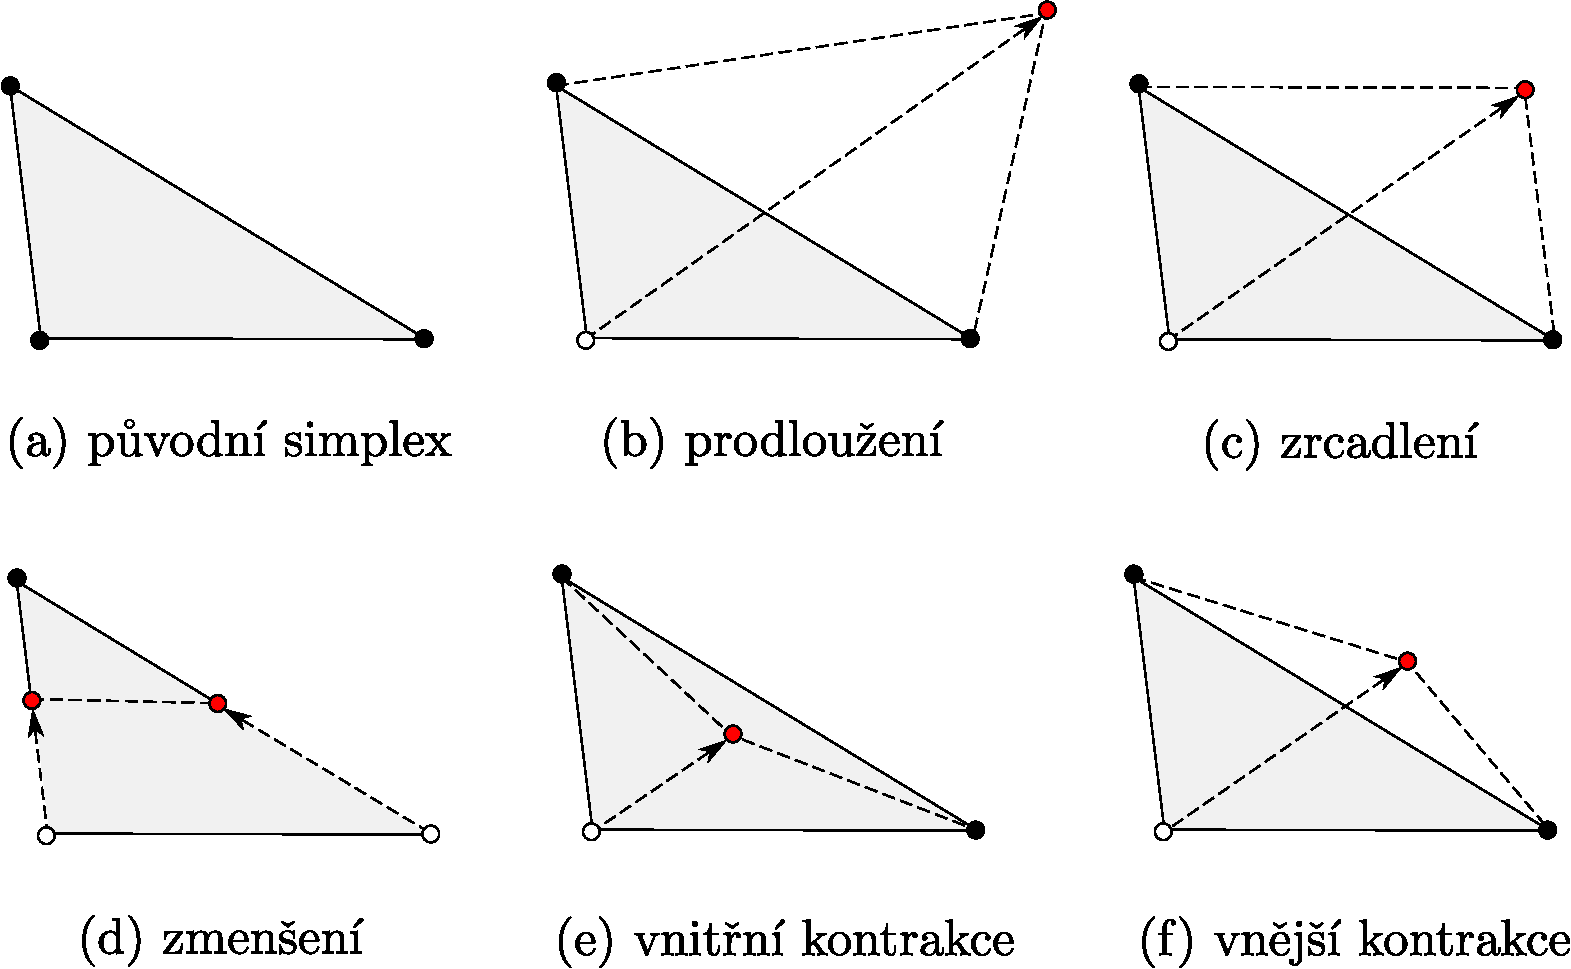
\includegraphics[width=0.76\textwidth]{Images/neldermead.pdf}
	\vspace{2mm}
	\caption{Schéma operací používaných k transformaci simplexů v rámci Nelderovy-Meadovy metody. Vrcholy vzniklé aplikací dané operace jsou vyznačeny červeně. Pro názornost jsou operace vyobrazeny v $ \mathbb{R}^2 $.}
	\vspace{2mm}
	\label{fig:NM operations}
\end{figure}


Heuristický charakter Nelderovy-Meadovy metody vyplývá z toho, že její princip je postaven na do jisté míry náhodném prohledávání prostoru pomocí předem definovaných pravidel. Několik iterací prohledávání prostoru pomocí simplexů je pro konkrétní volbu počátečního simplexu a konkrétní funkci znázorněno na obr. \ref{fig:NM}. Je dokázána konvergence této metody, není však zaručeno, že metoda vždy nutně konverguje ke stacionárnímu bodu \cite{BBO-textbook}. Podotkněme, že Nelderova-Meadova metoda je primárně odvozena pro optimalizaci úloh bez vazeb, lze však použít techniky popsané v sekci \ref{unconstrained} a použít ji pro optimalizaci úloh s vazbami.

%\begin{figure}[H]
%	\centering
%	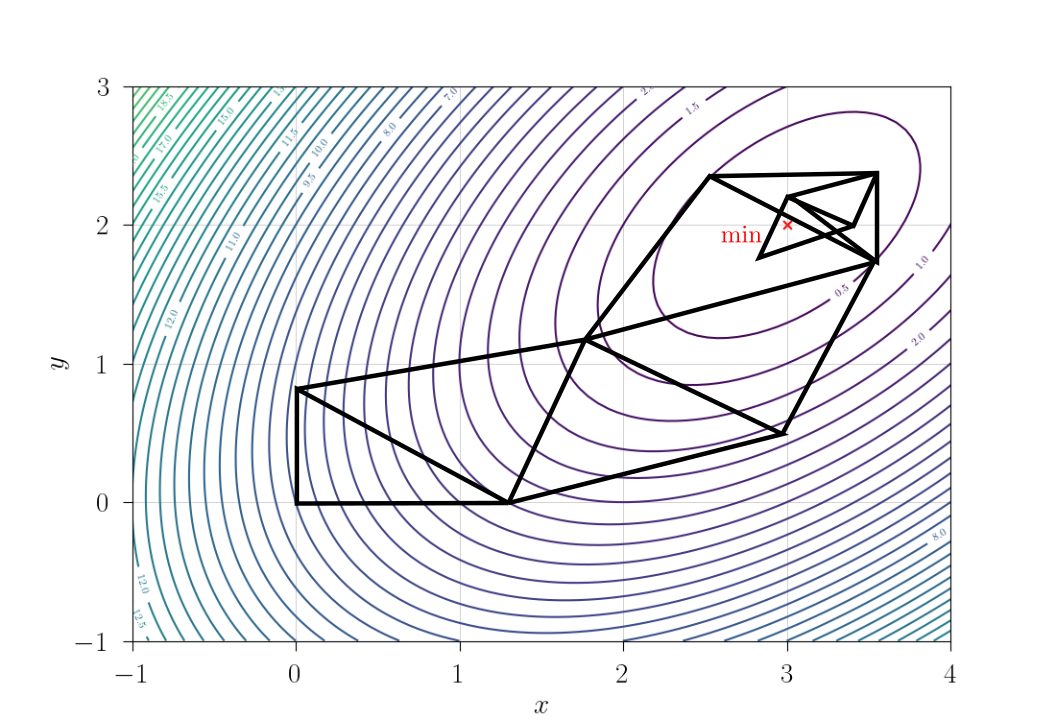
\includegraphics[width=0.99\textwidth]{Images/nelder.png}
%	\vspace{2mm}
%	\caption{Několik iterací Nelderovy-Meadovy metody pro konkrétní volbu počátečního simplexu při minimalizaci funkce $ x^2 - 4x + y^2 - y - xy + 7 $ s minimem v bodě (3,2) znázorněným červeným křížkem.}
%	\vspace{2mm}
%	\label{fig:NM}
%\end{figure}

\begin{figure}[H]
	\vspace{-2mm}
	\begin{subfigure}[b]{0.32\textwidth}
		\centering
%		trim={<left> <lower> <right> <upper>}
		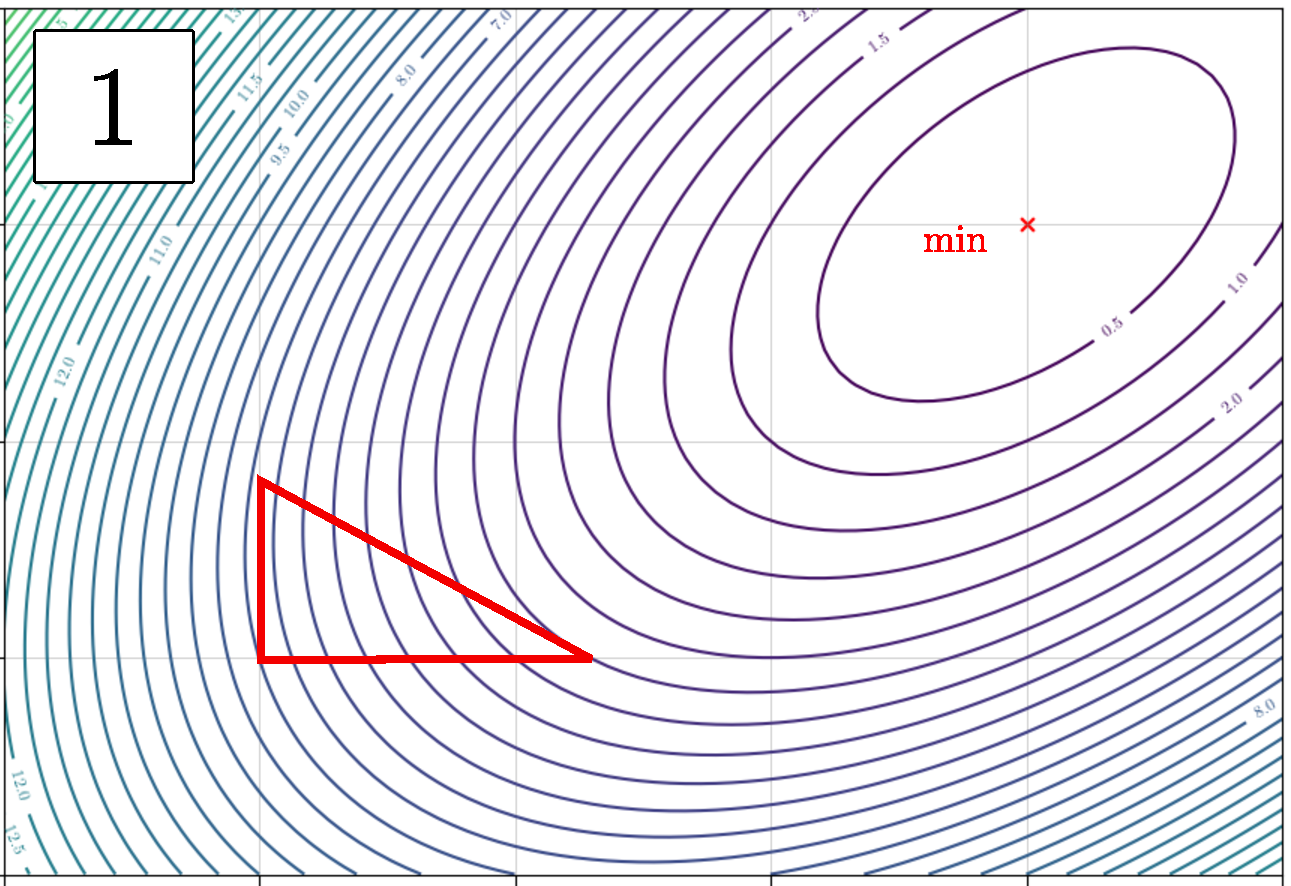
\includegraphics[width=0.96\textwidth, trim={0 0 0 0}, clip]{Images/nelder1.pdf}
	\end{subfigure}
	\begin{subfigure}[b]{0.32\textwidth}
		\centering
		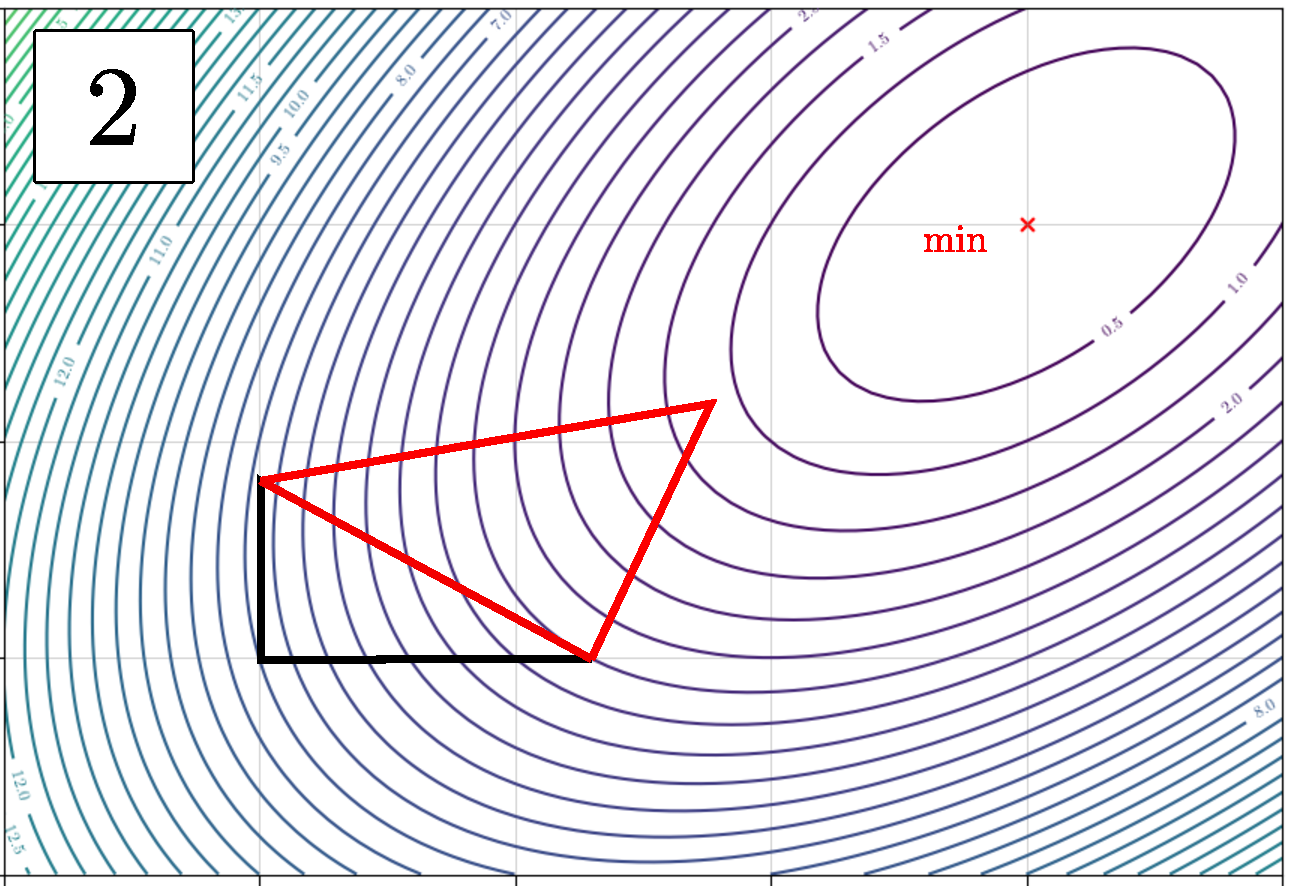
\includegraphics[width=0.96\textwidth, trim={0 0 0 0}]{Images/nelder2.pdf}
	\end{subfigure}
	\vspace{1mm}
	\begin{subfigure}[b]{0.32\textwidth}
		\centering
		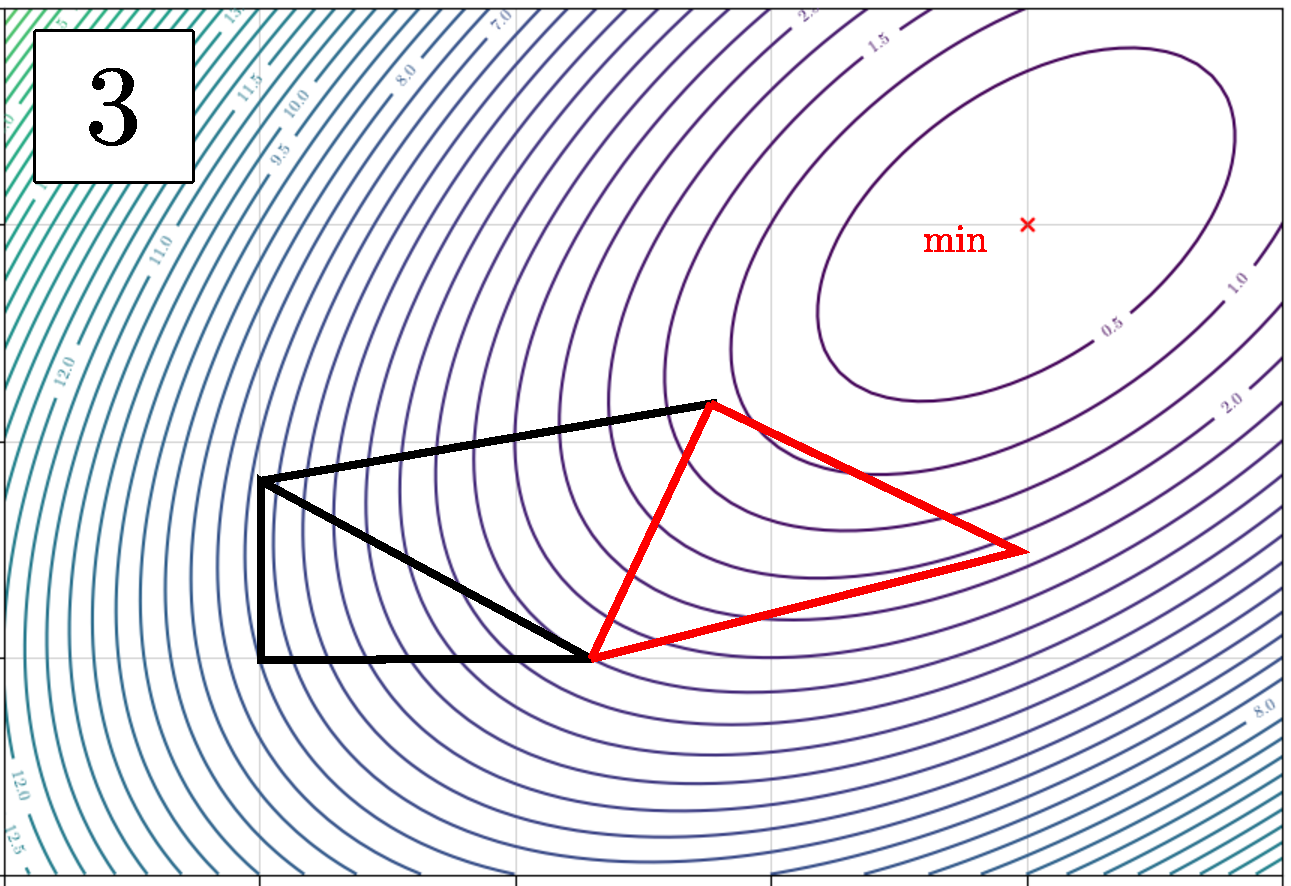
\includegraphics[width=0.96\textwidth, trim={0 0 0 0}]{Images/nelder3.pdf}
	\end{subfigure}
	\vspace{1mm}
	\begin{subfigure}[b]{0.32\textwidth}
		\centering
		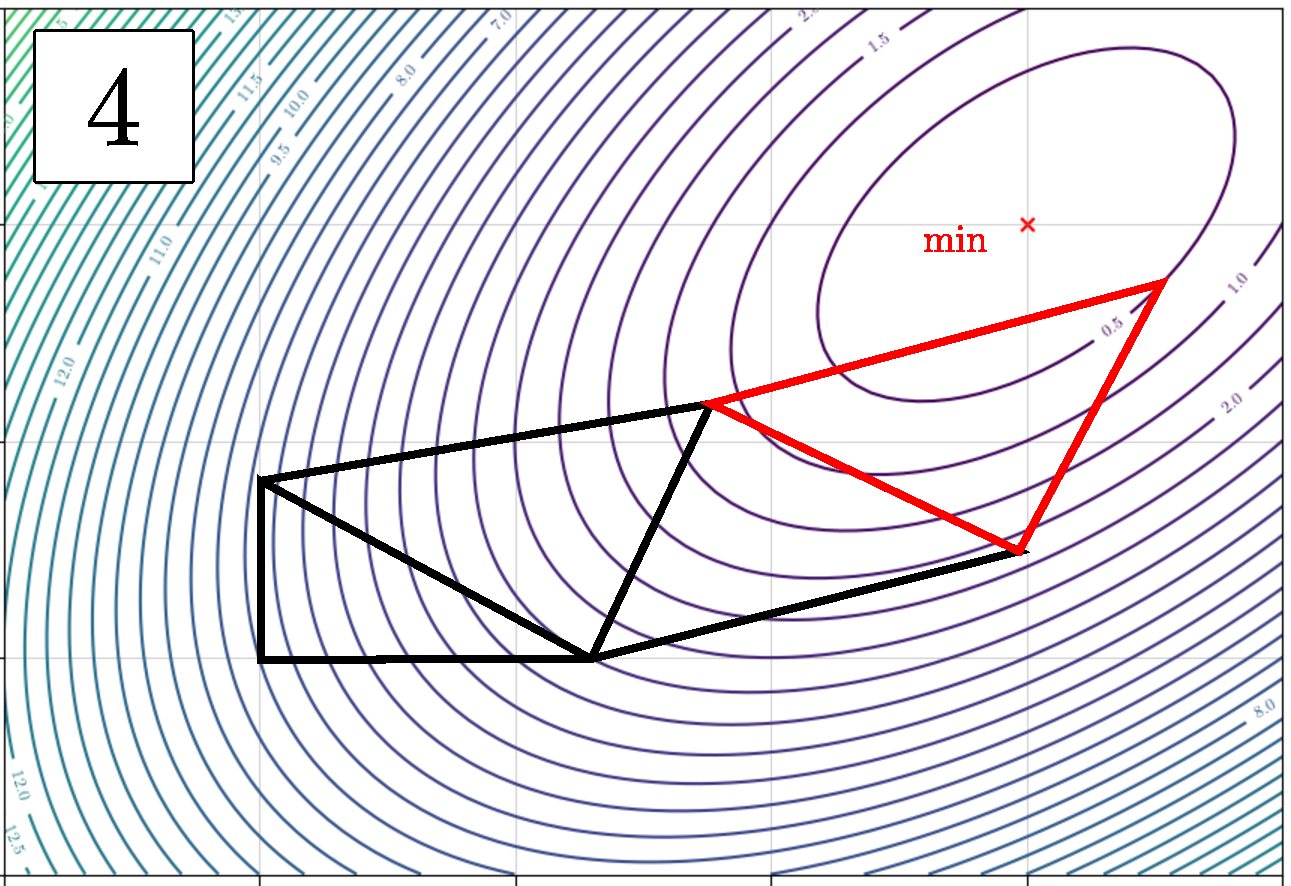
\includegraphics[width=0.96\textwidth, trim={0 0 0 0}]{Images/nelder4.pdf}
	\end{subfigure}
	\begin{subfigure}[b]{0.32\textwidth}
		\centering
		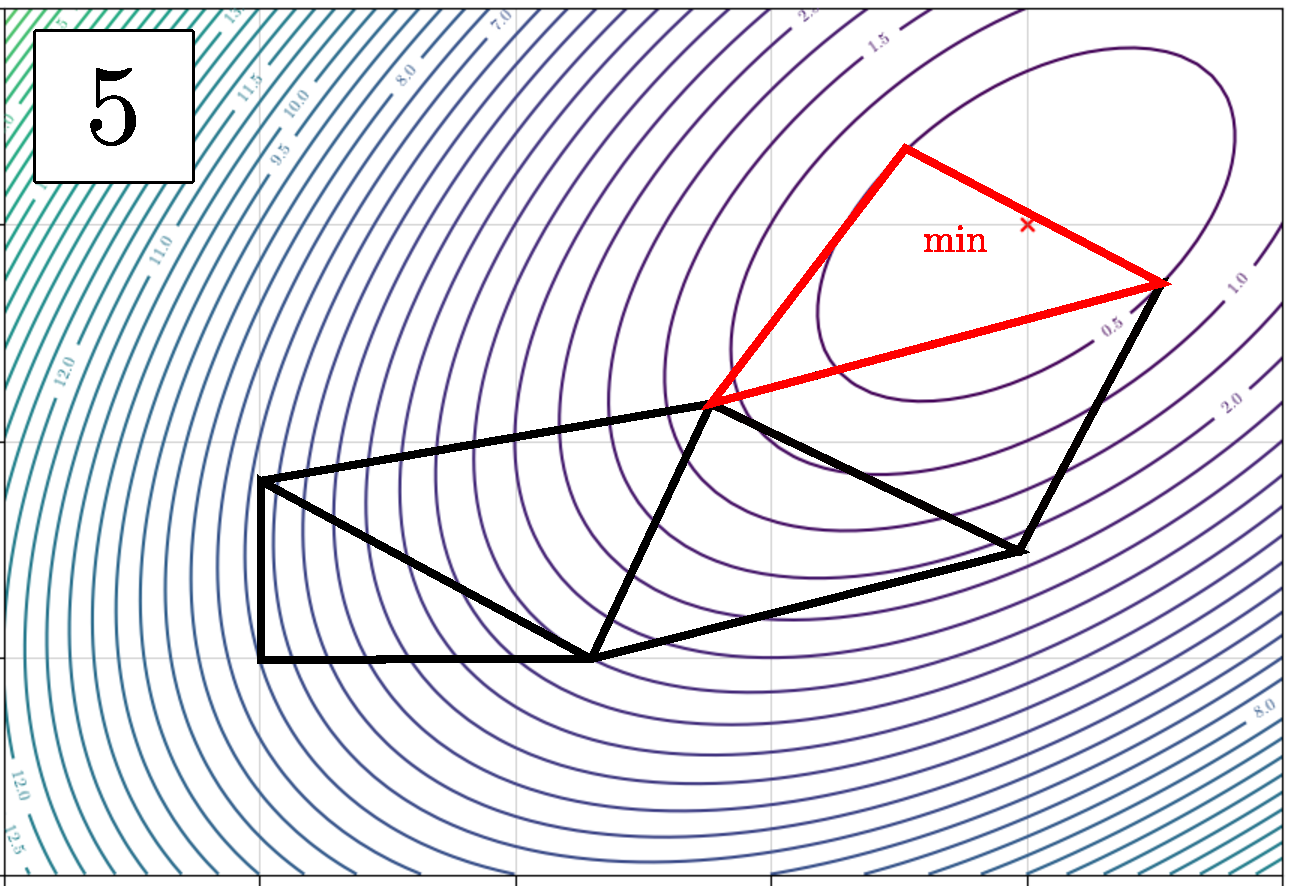
\includegraphics[width=0.96\textwidth, trim={0 0 0 0}]{Images/nelder5.pdf}
	\end{subfigure}
	\begin{subfigure}[b]{0.32\textwidth}
		\centering
		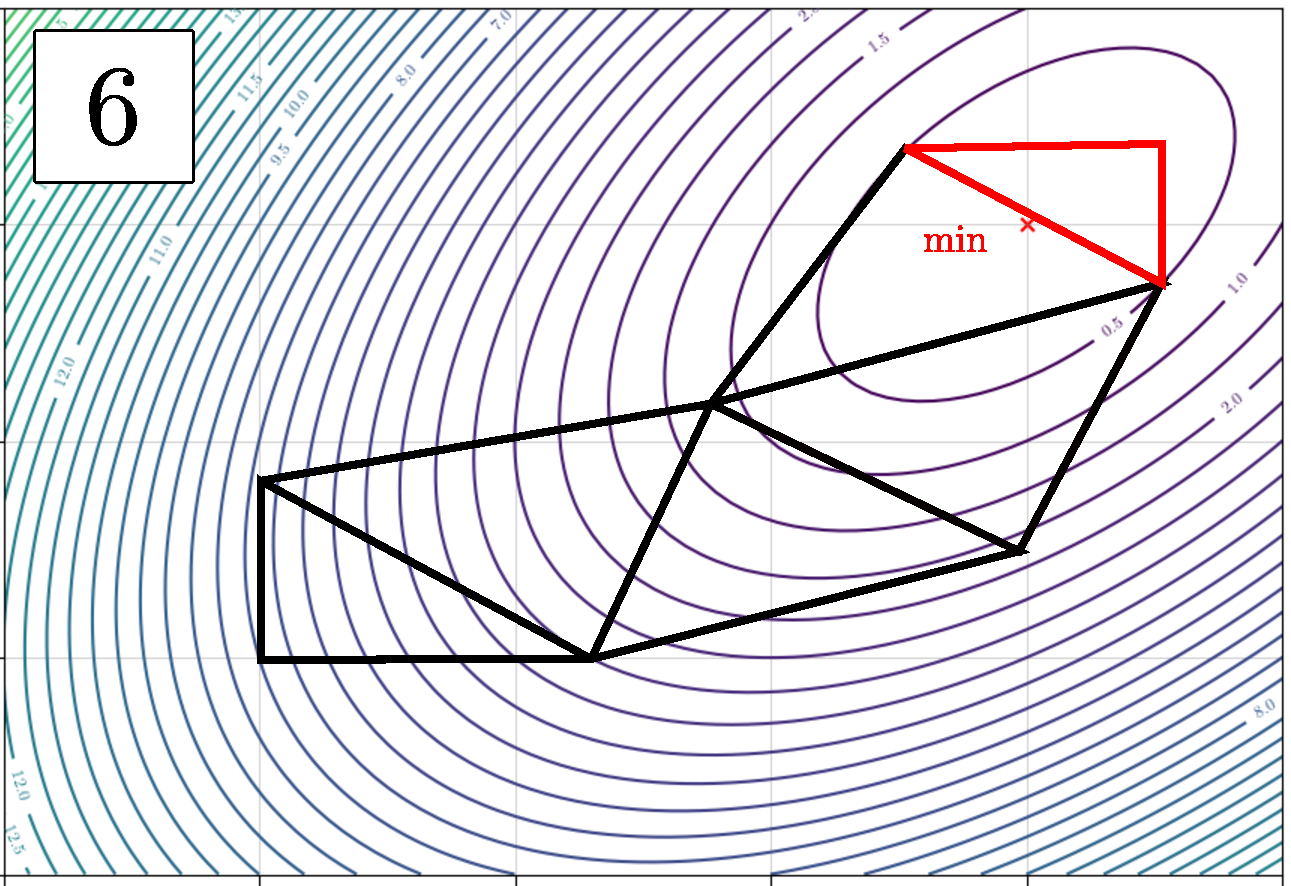
\includegraphics[width=0.96\textwidth, trim={0 0 0 0}]{Images/nelder6.pdf}
	\end{subfigure}
	\centering
	\begin{subfigure}[b]{0.32\textwidth}
		\centering
		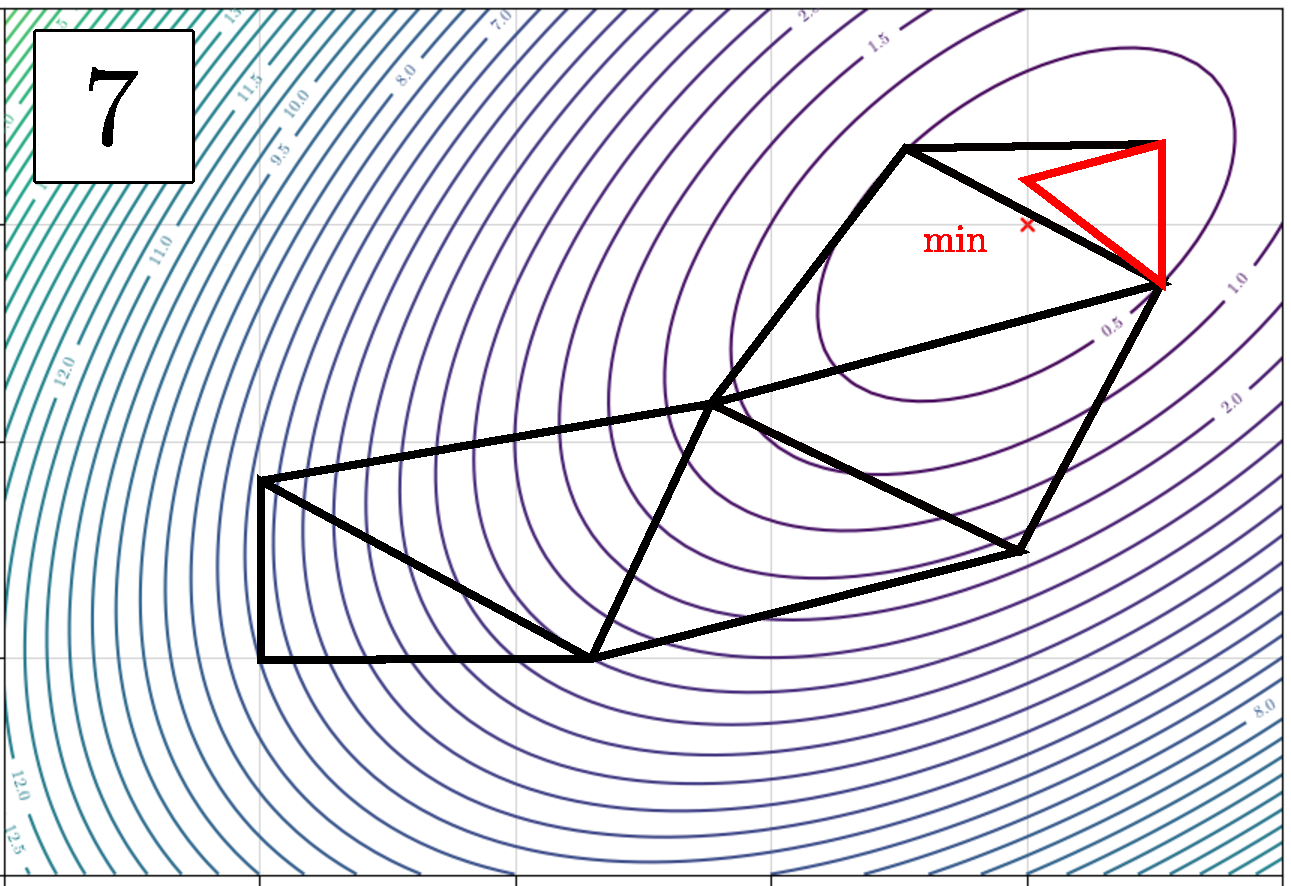
\includegraphics[width=0.96\textwidth, trim={0 0 0 0}]{Images/nelder7.pdf}
	\end{subfigure}
	\begin{subfigure}[b]{0.32\textwidth}
		\centering
		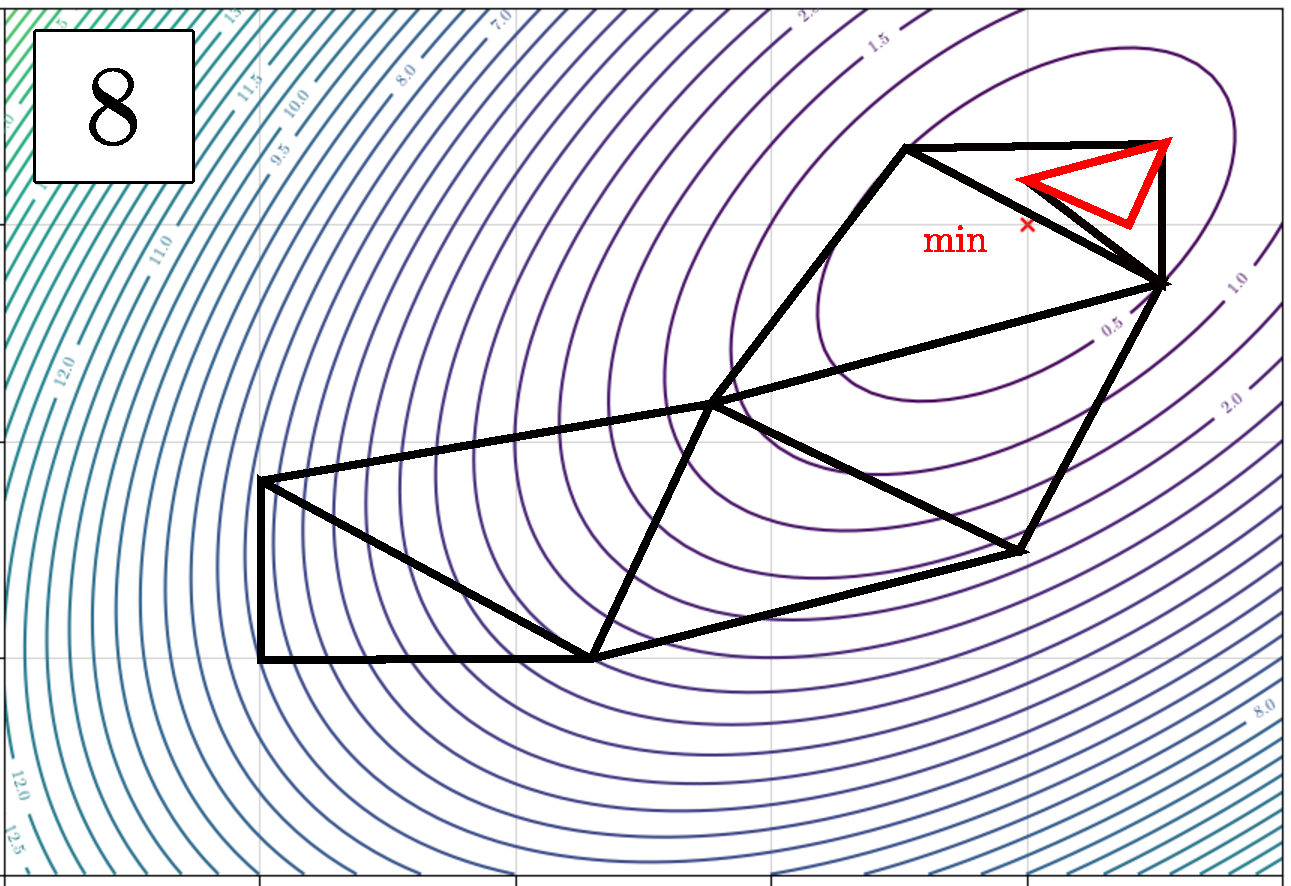
\includegraphics[width=0.96\textwidth, trim={0 0 0 0}]{Images/nelder8.pdf}
	\end{subfigure}
	\begin{subfigure}[b]{0.32\textwidth}
		\centering
		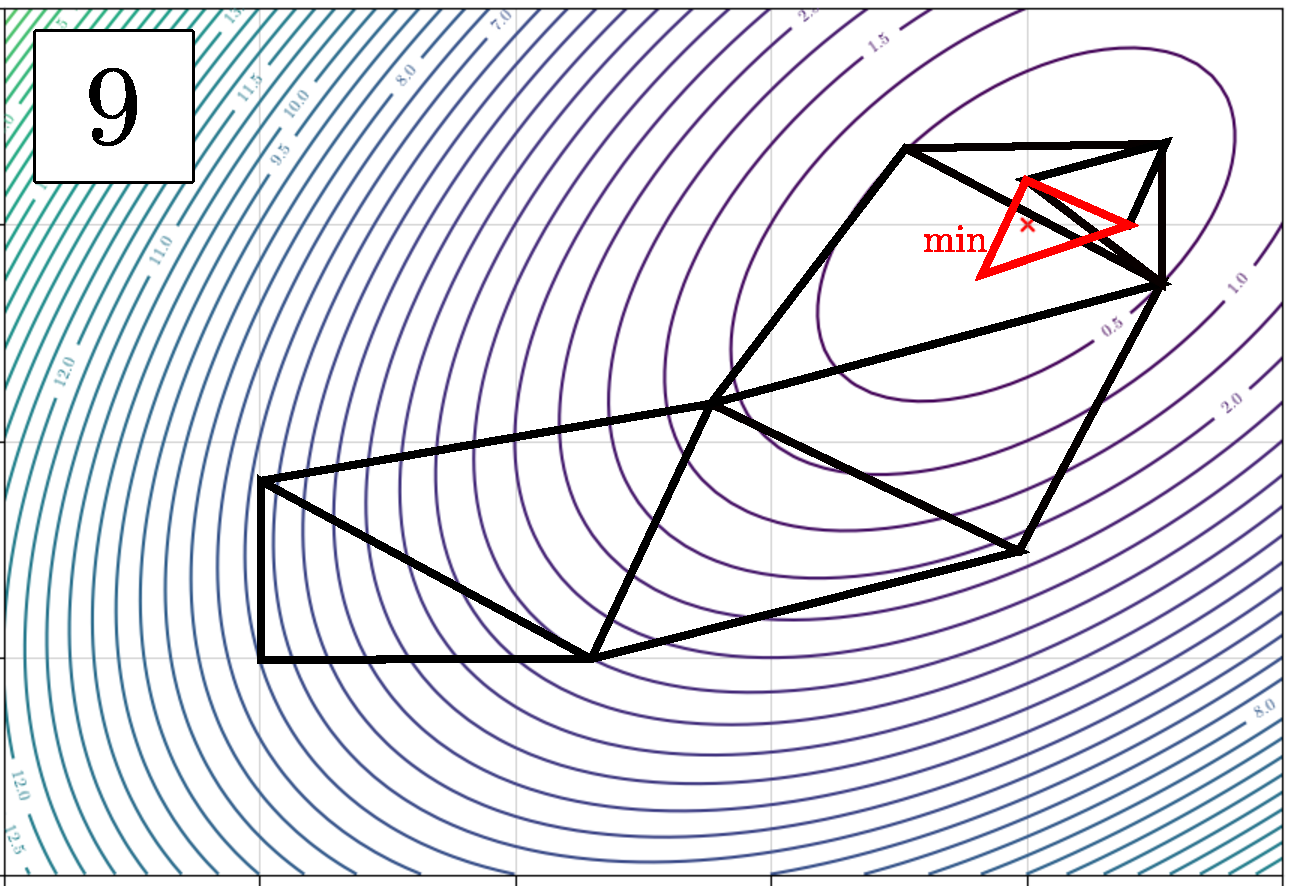
\includegraphics[width=0.96\textwidth, trim={0 0 0 0}]{Images/nelder9.pdf}
	\end{subfigure}
	\begin{center}
		\begin{subfigure}[b]{0.66\textwidth}
			\centering
			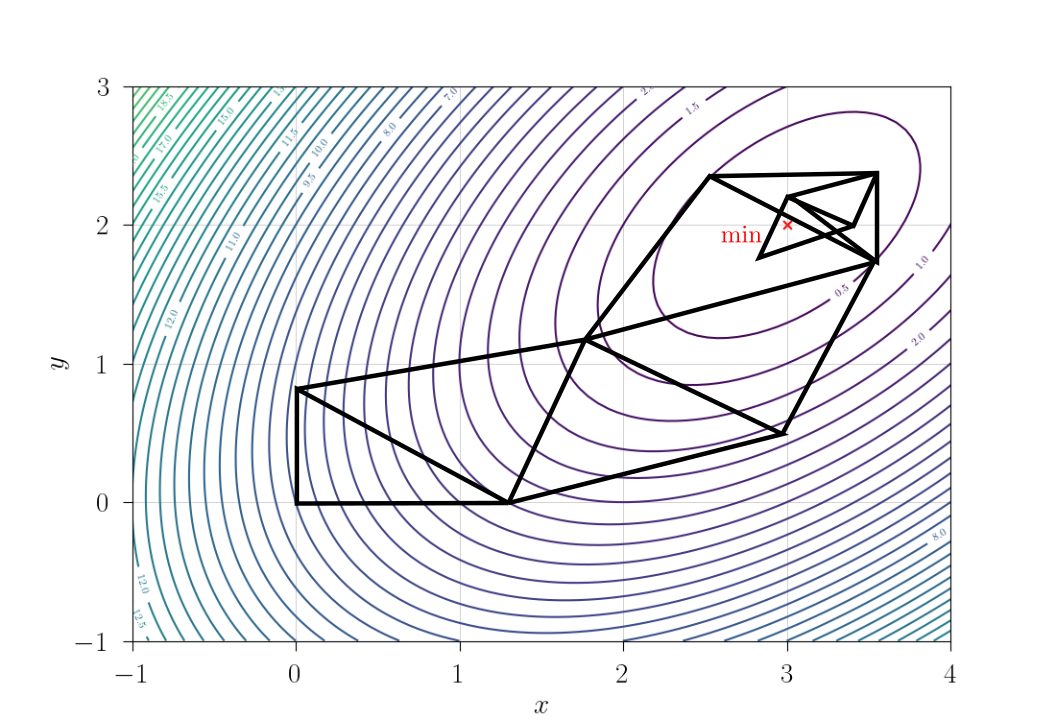
\includegraphics[width=0.985\textwidth, trim={0 6mm 0 9mm}]{Images/nelder.png}
		\end{subfigure}
	\end{center}

	\caption{Několik iterací Nelderovy-Meadovy metody pro konkrétní volbu počátečního simplexu při minimalizaci funkce $ x^2 - 4x + y^2 - y - xy + 7 $ s minimem v bodě (3,2) znázorněným červeným křížkem.}
	\label{fig:NM}
\end{figure}


\subsection{Metody přímého vyhledávání}\label{direct-search}
Z metod přímého vyhledávání popíšeme \textit{generalised pattern search} (dále jen GPS) metodu \cite{Audet2002} a~krátce zmíníme také \textit{mesh adaptive direct search} (dále jen MADS) metodu \cite{Audet2006}.

Pro popis algoritmu GPS je nutné definovat síť, pomocí níž je pak popsáno prohledávání prostoru v~rámci GPS. Buďte $ \mathbf{G} \in \mathbb{R}^{n \times n} $ a $ \mathbf{Z} \in \mathbb{Z}^{n \times p} $. Nechť  každý vektor z $ \mathbb{R}^{n} $ lze vyjádřit jako lineární kombinaci sloupců matice $ \mathbf{Z} $ (vnímaných jako vektory) tak, že všechny koeficienty v této lineární kombinaci jsou nezáporné. Dále označme $ \mathbf{S} = \mathbf{G} \mathbf{Z}$. Síť $ \mathbf{M} $ generovanou pomocí $ \mathbf{S} $ středovanou v bodě $ \vec{x} $ definujeme jako
\begin{equation}
	\mathbf{M} = \left\{ \vec{x} + \delta \, \mathbf{S} y \, | \, y \in \mathbb{N}^p \right\},
\end{equation}
kde $ \delta $ je parametr, jenž budeme nazývat síťový krok \cite{BBO-textbook, Audet2002}. V jednotlivých iteracích algoritmu GPS se obecně mění tvar sítě, jelikož je vždy středována v bodě představující nejlepší odhad v dané iteraci, dále se také mění velikost síťového kroku. Označíme-li $ \vec{x}_k $, resp. $ \delta_k $ jako odhad řešení, resp. síťový krok  v $ k $-té iteraci, můžeme definovat síť v $ k $-té iteraci označenou $ \mathbf{M} _k$, tj.
\begin{equation}
\mathbf{M} _k = \left\{ \vec{x}_k + \delta_k \, \mathbf{S} y \, | \, y \in \mathbb{N}^p \right\}.
\end{equation}
Poznamenejme, že sloupce výše definované matice $ \mathbf{S} $ lze chápat jako možné směry, kterými lze v rámci GPS prohledávat prostor hodnot optimalizačních parametrů \cite{BBO-textbook, Audet2002}.

Po inicializaci nutných počátečních parametrů je samotný algoritmus GPS v každé iteraci rozdělen do dvou hlavních kroků. Prvním krokem je tzv. hledání (anglicky \textit{search step}). Během kroku hledání je pomocí strategie blíže specifikované uživatelem vybrána konečná množina kandidátních síťových bodů, v nichž je vyčíslena účelová fukce. Pokud žádná z vypočtených hodnot nepředstavuje zlepšení oproti hodnotě $ f(\vec{x}_k) $, nastává krok průzkumu (anglicky \textit{poll step}). V kroku průzkumu je účelová funkce vyčíslena ve všech sousedních síťových bodech bodu $ \vec{x}_k $. V případě, že ani pak žádná z vypočtených hodnot nepředstavuje zlepšení oproti hodnotě $ f(\vec{x}_k) $, nastavíme $ \vec{x}_{k+1} = \vec{x}_k $ a snížíme hodnotu síťového kroku, tedy  $ \delta_{k+1} < \delta_k $. Pokud však v kroku hledání nebo v kroku průzkumu najdeme takový bod, pro který dojde k vylepšení odhadu řešení, označíme tento bod jako $ \vec{x}_{k+1} $ a zvýšíme hodnotu síťového kroku, tedy  $ \delta_{k+1} > \delta_k $ \cite{BBO-textbook, Audet2002}.

Výše popsané změny v každé iteraci vždy definují novou síť $ \mathbf{M} _k$, která se během algoritmu GPS obecně mění. Algoritmus je ukončen, když je splněno $ \delta_{k+1} < \varepsilon $ pro uživatelem specifikované $ \varepsilon > 0 $. Lze ukázat, že během GPS algoritmu konverguje krok sítě limitně k nule a za splnění vhodných předpokladů odhady řešení konvergují ke stacionárnímu bodu účelové funkce, detaily lze najít v \cite{BBO-textbook}. Podotkněme, že konvergence GPS je dokázána pro úlohy bez vazeb \cite{BBO-textbook}.

Dále krátce zmíníme metodu MADS, která představuje vylepšení metody GPS. Narozdíl od metody GPS, algoritmus MADS umožní během kroku průzkumu obecně zkoumat hodnoty účelové funkce ve směrech, které tvoří hustou podmnožinu v $ \mathbb{R}^{n} $ \cite{BBO-textbook, derivative-free-review}. Toto zobecnění vylepšuje konvergenci algoritmu a umožňuje dokázat konvergenci MADS i pro úlohy s vazbami, kdy je účelová funkce modifikována na extrémní bariérovou funkci \ref{eq:extreme barrier}. Detaily týkající se algoritmu a fungování metody MADS lze najít např.~v~\cite{BBO-textbook}.

\subsection{Optimalizace s využitím náhradního modelu}\label{model-based}
V případech, kdy je vyčíslení účelové funkce v konkrétním bodě časově nebo výpočetně  náročné, je užitečné během optimalizace v nějaké formě využít náhradu účelové funkce. Definujeme náhradní model (anglicky \textit{surrogate model}) zkoumané úlohy jako úlohu
\begin{equation}
	\min_{\vec{x} \in \mathbf{\tilde{X}}} \tilde{f}(\vec{x}),
\end{equation}
kde
\begin{equation}
\mathbf{\tilde{X}} = \big\{ \vec{x} \in \mathbf{D} \subseteq \mathbb{R}^n \ | \ \vec{\tilde{g}} (\vec{x}) \leq \vec{0} \wedge \vec{\tilde{h}} (\vec{x}) = \vec{0} \, \big\},
\end{equation}
přičemž funkce $ \tilde{f}, \vec{\tilde{g}}$ a $ \vec{\tilde{h}} $ mají podobný charakter, jako funkce $ f, \vec{g} $ a $ \vec{h}$ z původní úlohy. Charakter funkcí $ \tilde{f}, \vec{\tilde{g}}$ a $ \vec{\tilde{h}} $ je záměrně vymezen neurčitě - tento způsob definice odpovídá tomu, že po náhradním modelu nutně nepožadujeme, aby byl vhodným aproximativním modelem původní úlohy \cite{two-decades, BBO-textbook, Kramer2011}. Dobrý aproximativní model totiž nemusí být z hlediska optimalizace vhodnou náhradou, tato situace je znázorněna na obr. \ref{fig:surrogate}.

\begin{figure}[H]
	\centering
	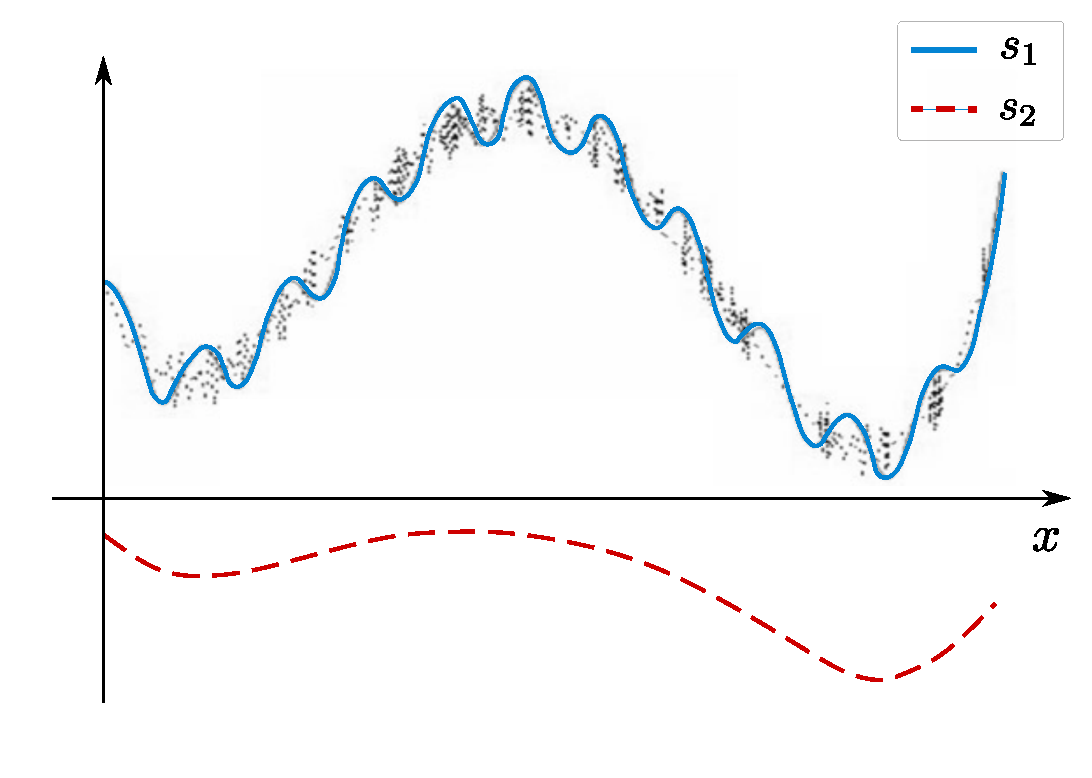
\includegraphics[width=0.6\textwidth]{Images/surrogate.pdf}
	\caption{Ilustrace dvou náhradních modelů $ s_1 $ a $ s_2 $. Černě jsou vyznačeny hodnoty účelové funkce vykazující šum. Použití náhradního modelu $ s_1 $ představuje volbu lepší z hlediska aproximace funkce, pro optimalizaci však tato volba vhodná není, jelikož $ s_1 $ obsahuje mnoho nežádoucích stacionárních bodů, které původní účelová funkce nemá. Na druhou stranu náhradní model $ s_1$ vhodně neaproximuje účelovou funkci ve smyslu funkčních hodnot, z hlediska optimalizace jde však o lepší volbu, jelikož stacionární body $ s_2$ se nacházejí na téměř shodných pozicích, jako je tomu u optimalizované účelové funkce.}
	\label{fig:surrogate}
\end{figure}

Využití náhradního modelu v rámci optimalizace je většinou dílčí částí jiné obecné optimalizační metody. Náhradní modely lze např. použít v rámci metod GPS a MADS popsaných v sekci \ref{direct-search}, kdy při vyčíslování účelové funkce v kroku průzkumu nejdříve vyčíslíme v těch samých bodech náhradní funkci $ \tilde{f} $, tyto hodnoty pak seřadíme, a již seřazenou množinu bodů použijeme k vyčíslení původní funkce $ f $. To nám umožní potenciálně výrazně zkrátit čas, který je potřebný k provedení kroku průzkumu, jelikož seřazením bodů zvýšíme pravděpodobnost, že úspěšně najdeme lepší odhad řešení již pro jeden z prvních zkoumaných bodů \cite{BBO-textbook}. Náhradní modely lze použít i v rámci jiných metod a urychlit tak jejich průběh, detailně je jejich použití rozebráno např. v \cite{two-decades, BBO-textbook}.


\section{Popis optimalizačního rámce}\label{ramec}
Pro použití popsaných optimalizačních metod v rámci problematiky dynamiky tekutin a numerických simulací je potřeba vytvořit plně automatizovaný optimalizační rámec. Je vhodné navrhnout takový rámec, jehož jednotlivé části budou dostatečně modulární, tedy v případě potřeby může být pro vykonání specifického úkonu v rámci procesu optimalizace snadno použita jiná metoda. Celkový navržený rámec zahrnuje několik částí, které dále popíšeme:

\begin{enumerate}
	\item \textit{Optimalizace}: První část zahrnuje samotnou použitou optimalizační metodu, která řídí celý další proces. V této části je definována řešená úloha společně s případnými požadovanými vazbami. Jak již bylo zmíněno, je vhodné, aby tato část byla co nejvíce nezávislá na ostaních částech popisovaného optimalizačního rámce. To nám dovolí použít různé metody implementované v jiných programovacích jazycích bez narušení chodu celkového procesu.
	
	V této práci budeme pracovat s metodami L-BFGS (viz sekce \ref{BFGS}) a Nelderovou-Meadovou metodou (viz sekce \ref{heuristic}). Pro implementeci obou těchto metod použijeme volně dostupný balík \texttt{Optim.jl} \cite{Optim.jl} implementovaný v programovacím jazyce Julia. Pro zahrnutí vazeb použijeme v obou případech metodu transformující účelovou funkci na extrémní bariérovou funkci, která byla pro účely této práce implementována nad rámec použitého balíku. Pro výpočet gradientu v rámci metody L-BFGS použijeme automatickou diferenciaci, která je dostupná v rámci balíku \texttt{Optim.jl} a jejíž detaily jsou popsány v \cite{Optim.jl}. Metodu L-BFGS s toutou volbou výpočtu gradientu budeme dále značit L-BFGS(A).
	
	Dále v rámci optimalizačního rámce zařazujeme metodu přímého vyhledávání MADS (viz sekce \ref{direct-search}) implementovanou v programovacím jazyce C++ ve volně dostupné knihovně \texttt{NOMAD} \cite{nomad}. Pro zarhnutí vazeb rovněž použijeme extrémní bariérovou funkci, která je v případě knihovny \texttt{NOMAD} její součástí. Podotkněme, že v rámci této práce metoda MADS není využita.
	
	\item \textit{Generování geometrie}: Optimalizační parametry, jejichž hodnota se v každé iteraci optimalizace mění, jsou předány do generátoru geometrie. Pro generování geometrie, která je dále využita v numerické simulaci, byl použit balík \texttt{meshgenerator} implementovaný v jazyce Python. Zmíněný balík vznikl pro účely této práce a je blíže popsán v kapitole \ref{geometrie}.
	
	\item \textit{Numerická simulace}: Poslední částí optimalizačního rámce je řešič umožňující vyčíslení optimalizované účelové funkce. V rámci této práce se zabýváme pouze problémy týkajícími se dynamiky tekutin. Pro numerickou simulaci proudění byla použita metoda LBM, která je společně s implementačními poznámkami popsána v kapitole \ref{lbm}.
	
\end{enumerate}
Schématicky je propojení jednotlivých částí optimalizačního rámce zobrazeno na obr. \ref{fig:framework}.

\begin{figure}[H]
	\vspace{8mm}
	\centering
	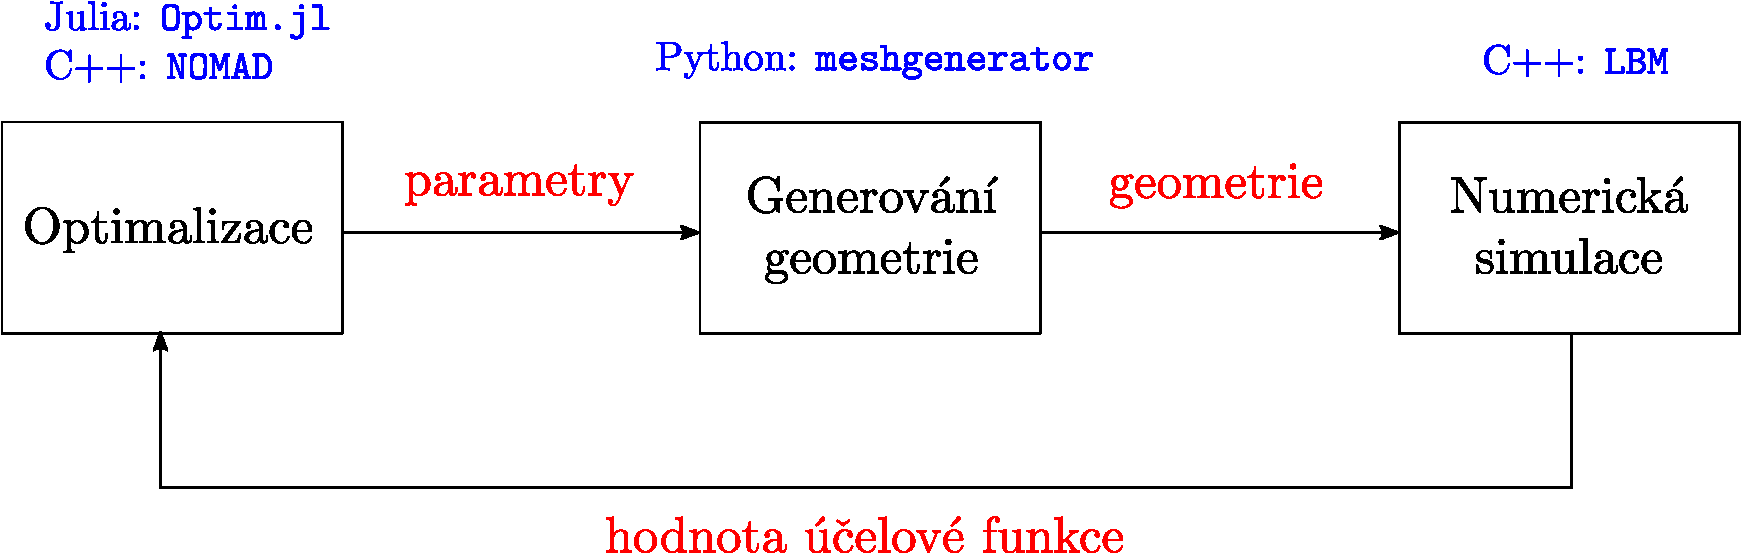
\includegraphics[width=0.85\textwidth]{Images/framework.pdf}
	\vspace{7mm}
	\caption{Schématické znázornění navrženého optimalizačního rámce. Šipkami je znázorněno propojení jednotlivých částí, nad šipkou je pak zdůrazněno, co jednotlivé části předávají v procesu dále.}
	\label{fig:framework}
\end{figure}

%\section{Poznámky k implementaci}\label{implementacni poznamky}
 
\chapter{Numerické výsledky}\label{vysledky}
V této kapitole uvedeme výsledky  provedených numerických simulací. Bude k nim využita mřížková Boltzmannova metoda popsaná v kapitole \ref{lbm} a bude uvažován matematický model pro nestlačitelnou tekutinu popsaný v kapitole~\ref{mmodel}. Hlavním cílem numerických simulací bude postupně ověřit fungování optimalizačního rámce popsaného v sekci \ref{ramec} a prozkoumat fungování možných optimalizačních metod. Po ověření funkčnosti optimalizačního rámce je dále cílem demonstrovat možnost formulovat netriviální optimalizační úlohy a následně je řešit. Postupně budeme řešit úlohy s jedním, dvěma a třemi optimalizačními parametry vždy s různou uvažovanou geometrií, což bude demonstrovat možná použití balíku \texttt{meshegenerator}.


\section{Úlohy s jedním optimalizačním parametrem}
\subsection{Definice parametrů úlohy}
Uvažujeme dvourozměrnou oblast $ \Omega $ s rozměry $ \left(0; 5H\right) \times \left(0; H\right)$, kde $ H = 0{,}5 \, \mathrm{m} $. Tuto oblast dále rozdělíme na pět částí stejného rozměru - prostřední tři části označíme postupně A, B a C. V části B bude v rámci úloh vždy umístěn objekt, jehož geometrie se během procesu optimalizace mění. V části A bude dle potřeby umístěn objekt neměnný během procesu optimalizace, který bude sloužit k případnému vytvoření netriviálního rychlostního profilu v rámci oblasti. V části C pak bude vyhodnocována zvolená optimalizovaná účelová funkce. Definice a rozdělení výpočetní oblasti na části je znázorněno na obr. \ref{fig:oblast uloha 1}.
\begin{figure}[H]
	\vspace{2mm}
	\centering
	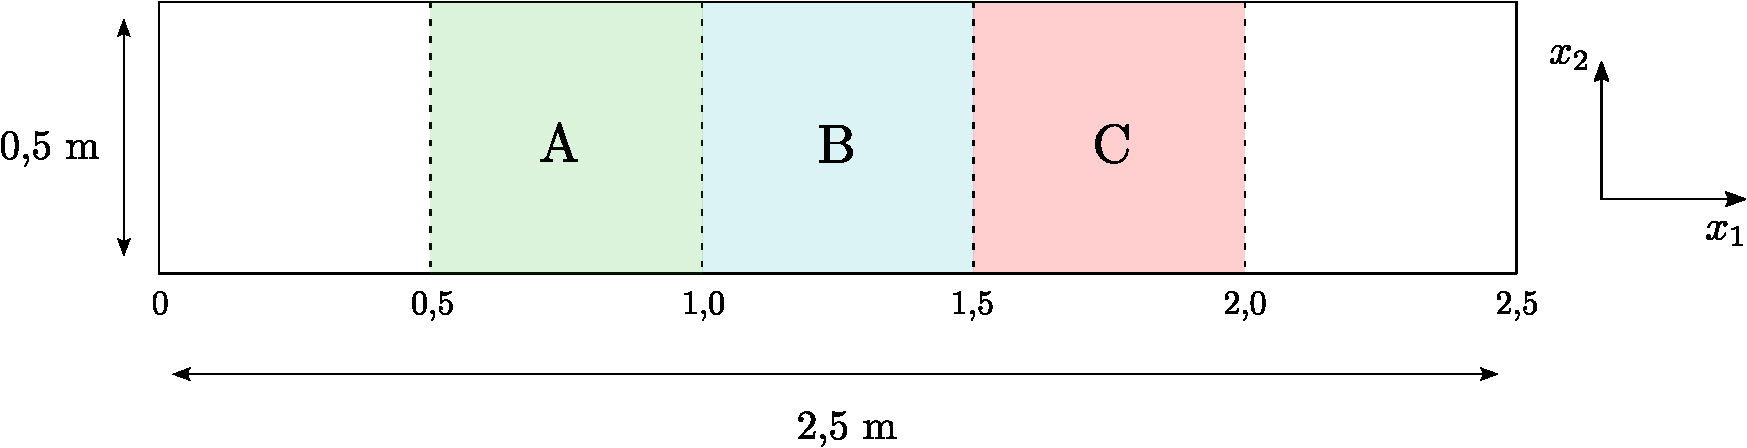
\includegraphics[width=1.0\textwidth]{Images/oblast12.pdf}
	\caption{Schématické znázornění definice a rozdělení výpočetní oblasti.}
	\label{fig:oblast uloha 1}
\end{figure}


Rychlost na vstupu budeme předepisovat parabolickým profilem ve tvaru
\begin{equation}\label{eq:parabolic inflow}
u_{1} \left(\vec{x}, t\right) = 4 U^{}_{m} \frac{x^{}_{2}}{H} \left(1 - \frac{x^{}_{2}}{H}\right), \hspace{3mm} u_{2} \left(\vec{x}, t\right) = 0, \hspace{4mm} \vec{x} \in \partial \hat{\Omega}_{\mathrm{in}},
\end{equation}
kde $ U^{}_{m}$ \si{[ms^{-1}]} je maximální požadovaná rychlost na parabolickém profilu.


\subsection{Rotující elipsa bez překážky}
\begin{uloha}{Základní úloha rotující elipsy}
	\vspace{2mm}
	Nastavení úlohy:
	\begin{itemize}
		\item $ \Omega=(0 ; 2{,}5 \mathrm{~m}) \times(0 ; 0{,}5 \mathrm{~m})$
		\item $ \nu=10^{-3} \mathrm{~m}^{2} \mathrm{~s}^{-1}$
	\end{itemize} 
	Nastavení v rámci LBM:
	\begin{itemize}
		\item Na $ \overline{\hat{\Omega}} $ volíme počáteční podmínku podle sekce \ref{pocatecni podminka}.
		\item Na $ \partial \hat{\Omega}_{\mathrm{W}} $ volíme rychlost podle vztahu \eqref{eq:parabolic inflow} s $ U_m = 2{,}5 $ \si{m s^{-1}}.
		\item Na jednotlivých částech hranice $ \partial \hat{\Omega}$ předepisujeme momentovou okrajovou podmínku popsanou v sekci \ref{moment based bc}. Na hranici obtékaného objektu v oblasti B předepisujeme Bouzidiho interpolační podmínku rozebranou v sekci \ref{interpolation bc}.
		\item Mřížku volíme jako $\overline{\hat{\Omega}} = N_{x} \times N_{y}$, $N_{x} = 1120, \, N_{y} = 224$,
		\item Kinematickou viskozitu v mřížkových jednotkách volíme $\nu^{L} = 10^{-3} $.
	\end{itemize}
	Použité objekty:
	\begin{itemize}
		\item V oblasti B je předepsán objekt třídy \texttt{Ellipse} popsaný v sekci \ref{meshgenenator}.
	\end{itemize} 
	Použité optimalizační metody:
	\begin{itemize}
		\item Použijeme L-BFGS(A) a Nelderovu-Meadovu metodu (NM), obě metody jsou popsány v kapitole~\ref{optimalizace}.
	\end{itemize}
	\label{ulo:1}
\end{uloha}

\begin{figure}[H]
	\centering
	\vspace{8mm}
	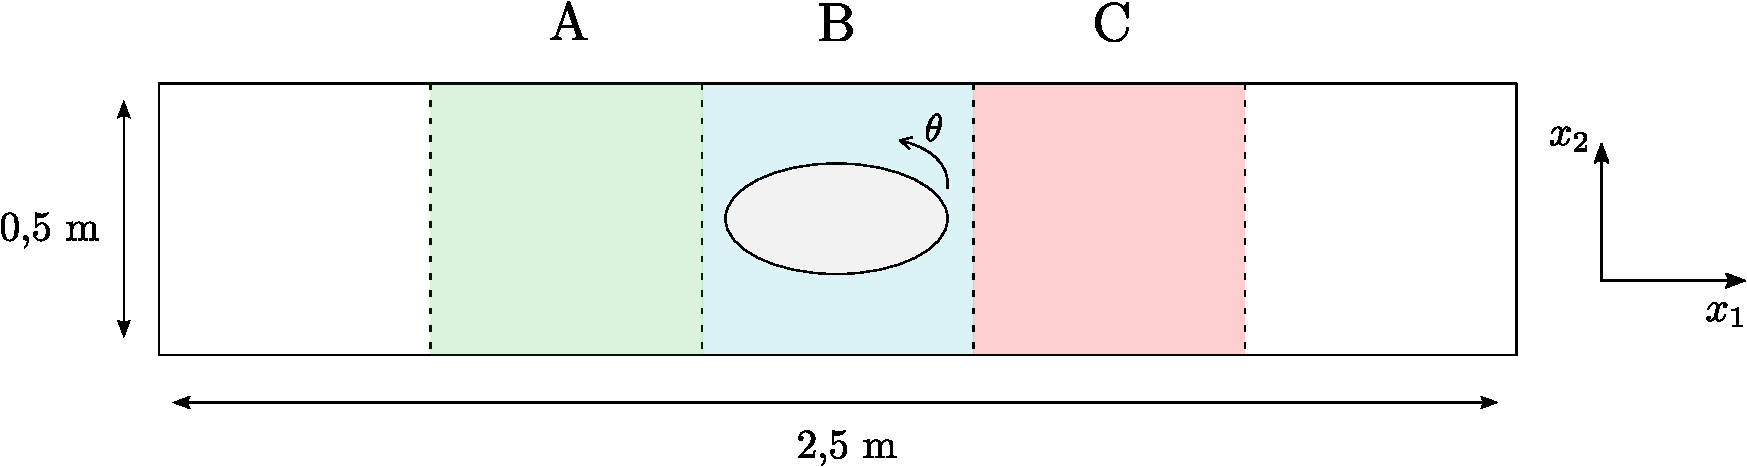
\includegraphics[width=1.0	\textwidth]{Images/elipsa1.pdf}
	\vspace{2mm}
	\caption{Schématické znázornění definice výpočetní oblasti v úloze 5.1.}
	\label{fig:elipsa 1}
	\vspace{1.8mm}
\end{figure}

V této úloze bude naším cílem zejména ověřit funkčnost optimalizačního rámce. Do oblasti B umístíme elipsu popsanou rovnicí
\begin{equation}
	\frac{(x-x_s)^2}{a^2} + \frac{(y-y_s)^2}{b^2} = 1,
\end{equation}
kde $ a = 0{,}21, \, b = 0{,}105, \, x_s = 1{,}25$ a $ y_s = 0{,}25 $, kde všechny uvedené parametry mají rozměr \si{[m]}. Umožníme definované elipse rotovat kolem svého středu v rozsahu úhlu $0^\circ \leq \theta \leq 180^\circ$, nastavení je schematicky znázorněno na obr. \ref{fig:elipsa 1}.

Označíme turbulentní kinetickou energii (definovanou pomocí \eqref{eq:turb kin energy}) v oblasti C závislou na úhlu~$ \theta $ jako $ T^{\text{C}}_{\text{turb}} (\theta) $. Naším cílem bude maximalizovat, resp. minimalizovat $ T^{\text{C}}_{\text{turb}} (\theta) $ za již zmíněného předpokladu $0^\circ \leq \theta \leq 180^\circ$.

Hodnoty účelové funkce jsou závislé na výsledku numerické simulace, tj. neznáme explicitní funkční předpis účelové funkce. Jedná se však o úlohu s pouze jedním optimalizačním parametrem na omezeném intervalu - můžeme definovat ekvidistatní dělení tohoto intervalu $ k, k=0,1,\dots,180$ a v dělících bodech účelovou funkci pomocí numerických simulací vyčíslit. Tyto hodnoty můžeme pak lineárně interpolovat, díky čemuž získáme představu o průběhu účelové funkce na uvažovaném intervalu. Interpolované hodnoty jsou společně s jejich maximem, resp. minimem zobrazeny na obr. \ref{fig:interpolovana elipsa 1}. Můžeme vidět, že maximum interpolované funkce je nabýváno při hodnotě $ \theta = 90^\circ $ - tedy očekáváme, že k maximálním turbulencím za překážkou bude docházet v případě, kdy překážka (elipsa) v největší míře přehradí oblast. Naopak minimum se nachází v bodě $ \theta = 0^\circ $, resp. $ \theta = 180^\circ $- tedy očekáváme, že k miminálním turbulencím za překážkou bude docházet v případě, kdy je překážka orientovaná ve směru proudění tekutiny. Podotkněme, že orientace elipsy je v těchto bodech stejná a tedy je stejná i hodnota interpolované funkce v~těchto bodech.

\begin{figure}[H]
	\centering
	\vspace{-2mm}
	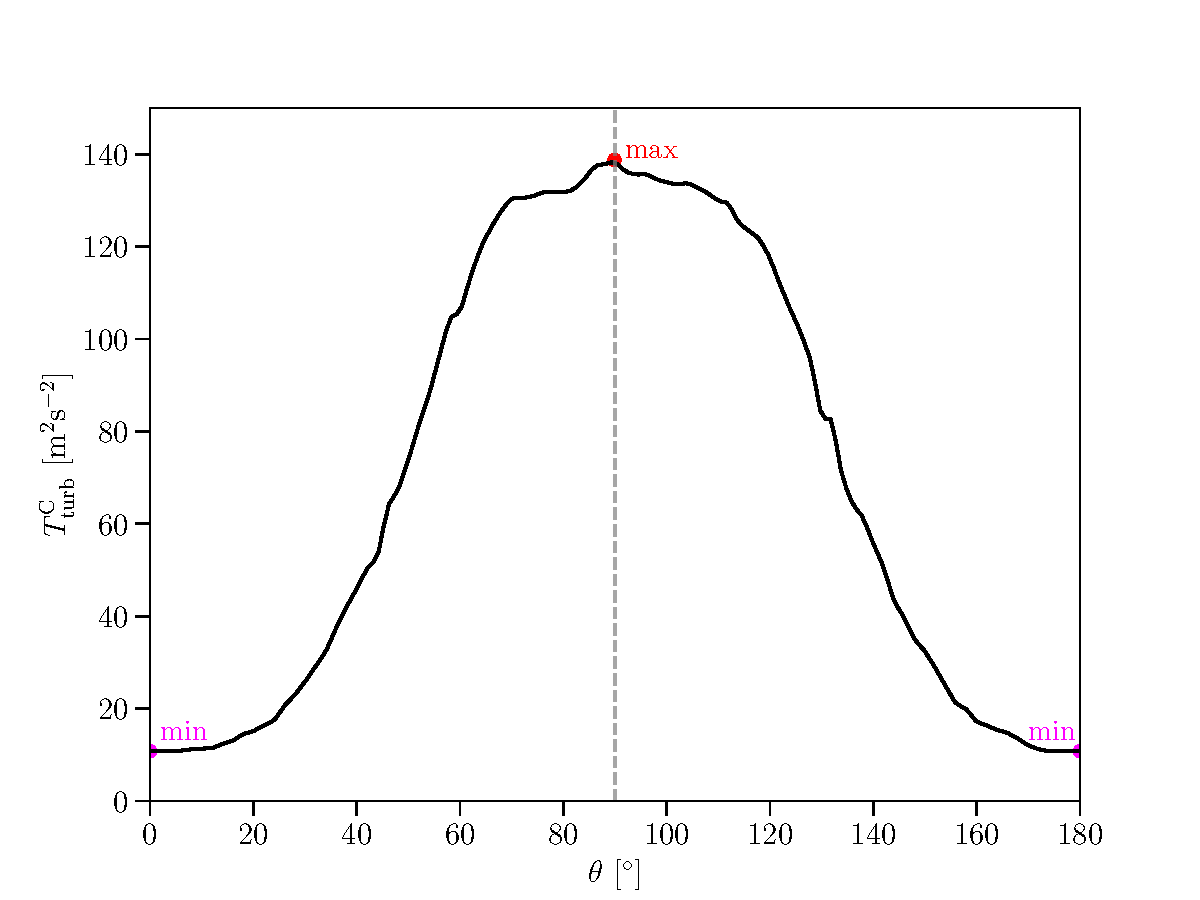
\includegraphics[width=0.82\textwidth]{Images/elip1interpolated.pdf}
	\vspace{2mm}
	\caption{Interpolované hodnoty pro úlohu 5.1 s vyznačeným maximem sloužící k následné jednodušší analýze výsledků.}
	\label{fig:interpolovana elipsa 1}
	\vspace{1.8mm}
\end{figure}

Zdůrazněme, že v rámci optimalizace využíváme pouze hodnoty z numerických simulací pomocí LBM (tj. optimalizační algoritmus nemá přístup k interpolovaným hodnotám), interpolované hodnoty nám však pomohou s následnou analýzou výsledků.

Zaveďme množinu
\begin{equation}\label{mnozina poc bodu}
	L = \big\{ 30 i \: | \: i = 0, 1, \dots, 6 \, \big\},
\end{equation}
která bude představovat počáteční body pro použité optimalizační metody. Záměrně mezi testované počáteční body zařazujeme i krajní hodnoty z intervalu přípustných řešení, abychom otestovali implementaci extrémní bariérové funkce. Prvky množiny $ L $ tedy představují počáteční body pro minimalizaci a maximalizaci.

Výsledky minimalizace, resp. maximalizace jsou k nahlédnutí v tabulce \ref{tab:elip1min}, resp. v tabulce \ref{tab:elip1max}, kde výsledný bod nalezený pomocí optimalizační metody značíme $\mathbf{x^\star}$. Body nalezené minimalizací, resp. maximalizací jsou znázorněny mezi interpolovanými hodnotami na obr. \ref{fig:elip1minbody}, resp. \ref{fig:elip1maxbody}. Z důvodu časové náročnosti numerických simulací je pro nás při posuzování vhodnosti použité metody stěžejní, kolikrát musela být během optimalizace vyčíslena účelová funkce - tuto hodnotu budeme značit $ \# f$ a je rovněž uvedena v tabulkách \ref{tab:elip1min} a \ref{tab:elip1max}. Dále je na obr. \ref{fig:elip1_0}, resp. \ref{fig:elip1_90} zobrazeno pole středních hodnot fluktuací pro případ s minimální, resp. maximální turbulentní kinetickou energií.

\begin{minipage}{\textwidth}
	\hspace{-3mm}
	\begin{minipage}[b]{0.4\textwidth}
		\bgroup
		\setlength\tabcolsep{3mm}
		\def\arraystretch{1.7}%
		$$
		\begin{array}{ccc}
		\hline \text { Označení bodu } & \theta \, [^{\circ}] & T^{\text{C}}_{\text{turb}} (\theta) \, [\text{m}^{2} \text{s}^{-2}] \\
		\hline
		A_{\min} & 0{,}00 & 10{,}72 \\
		B_{\min} & 180{,}00 & 10{,}72 \\
		C_{\min} & 174{,}24 & 10{,}74 \\
		\hline
		\end{array}
		$$
		\egroup
	\end{minipage}%
	\begin{minipage}[b]{0.16\textwidth}
	\centering
	\hspace{-4mm}
	\end{minipage}%
	\begin{minipage}[b]{0.4\textwidth}
		\bgroup
		\setlength\tabcolsep{3mm}
		\def\arraystretch{1.7}%
		$$
		\begin{array}{ccc}
		\hline \text { Označení bodu } & \theta \, [^{\circ}] & T^{\text{C}}_{\text{turb}} (\theta) \, [\text{m}^{2} \text{s}^{-2}] \\
		\hline
		A_{\max} & 90{,}00 & 138{,}75 \\
		B_{\max} & 77{,}21 & 131{,}94 \\
		C_{\max} & 95{,}58 & 135{,}84 \\
		\hline
		\end{array}
		$$
		\egroup
	\end{minipage}
\vspace{4mm}
    \hfill
\end{minipage}

\begin{minipage}{\textwidth}
	\begin{minipage}[b]{0.4\textwidth}
		\bgroup
		\setlength\tabcolsep{3mm}
		\def\arraystretch{1.5}%
		\begin{tabular}{|r|cc|cc|}
			\hline
			& \multicolumn{2}{c|}{L-BFGS(A)} & \multicolumn{2}{c|}{NM} \\ \hline
			\multicolumn{1}{|c|}{$\mathbf{x_0}$}& $\mathbf{x^\star}$ & $ \boldsymbol{\#f} $ & $\mathbf{x^\star}$ & $ \boldsymbol{\#f} $ \\ \hline
			$ 0^\circ $ 		&      A$_{\min}$           &     41   &    A$_{\min}$   &  12 \\ 
			$ 30^\circ $ 		&      A$_{\min}$     		&     41   &    A$_{\min}$   &  35 \\ 
			$ 60^\circ $ 		&      A$_{\min}$     		&     58   &    A$_{\min}$   &  33 \\ 
			$ 90^\circ $ 		&      B$_{\min}$     		&     31   &    C$_{\min}$   &  27 \\ 
			$ 120^\circ $ 		&      B$_{\min}$     		&     41   &    B$_{\min}$   &  31 \\ 
			$ 150^\circ $ 		&      B$_{\min}$     		&     37   &    C$_{\min}$   &  23 \\
			$ 180^\circ $ 		&      B$_{\min}$     		&     77   &    A$_{\min}$   &  7 \\ \hline
		\end{tabular}
		\vspace{2mm}
		\captionof{table}{Výsledky pro minimalizační úlohu s použitím metod L-BFGS(A) a~NM.}
		\label{tab:elip1min}
		\egroup
	\end{minipage}%
	\begin{minipage}[b]{0.15\textwidth}
		\centering
		\hspace{1mm}
	\end{minipage}%
	\begin{minipage}[b]{0.4\textwidth}
		\bgroup
		\setlength\tabcolsep{3mm}
		\def\arraystretch{1.5}%
		\begin{tabular}{|r|cc|cc|}
			\hline
			& \multicolumn{2}{c|}{L-BFGS(A)} & \multicolumn{2}{c|}{NM} \\ \hline
			\multicolumn{1}{|c|}{$\mathbf{x_0}$}& $\mathbf{x^\star}$ & $ \boldsymbol{\#f} $ & $\mathbf{x^\star}$ & $ \boldsymbol{\#f} $ \\ \hline
			$ 0^\circ $ 		&      B$_{\max}$           &     98   &    A$_{\max}$   &  45 \\ 
			$ 30^\circ $ 		&      A$_{\max}$     		&     42   &    A$_{\max}$   &  27 \\ 
			$ 60^\circ $ 		&      A$_{\max}$     		&     33   &    A$_{\max}$   &  21 \\ 
			$ 90^\circ $ 		&      A$_{\max}$     		&     9    &    A$_{\max}$   &  27 \\ 
			$ 120^\circ $ 		&      A$_{\max}$     		&     39   &    A$_{\max}$   &  26 \\ 
			$ 150^\circ $ 		&      A$_{\max}$     		&     36   &    A$_{\max}$   &  26 \\
			$ 180^\circ $ 		&      C$_{\max}$     		&     122  &    A$_{\max}$   &  28 \\ \hline
		\end{tabular}
		\vspace{2mm}
		\captionof{table}{Výsledky pro maximalizační úlohu s použitím metod L-BFGS(A) a~NM.}
		\label{tab:elip1max}
		\egroup
	\end{minipage}
	\hfill
\end{minipage}

\begin{figure}[H]
	\vspace{2mm}
	\begin{subfigure}[b]{0.45\textwidth}		
		\centering
		\hspace{-15mm}
		%		trim={<left> <lower> <right> <upper>}
		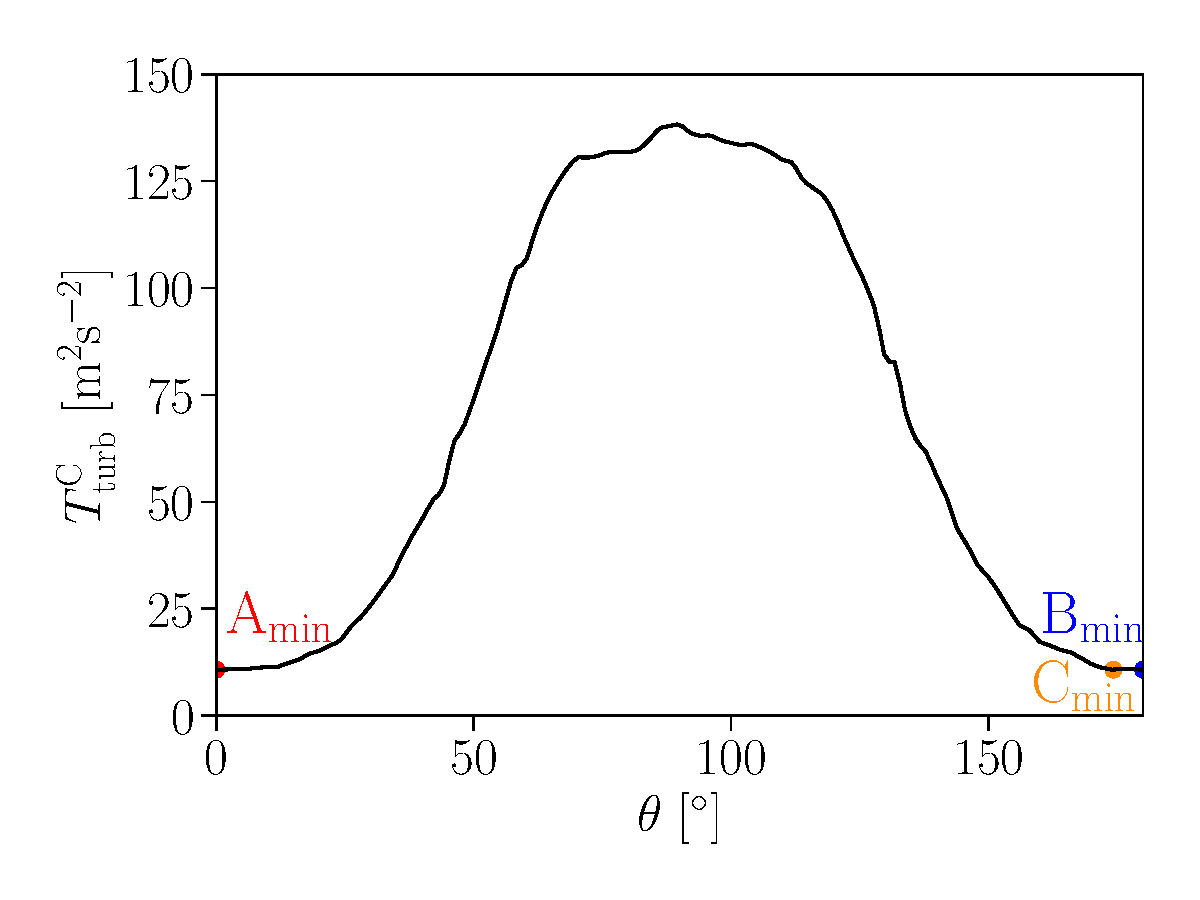
\includegraphics[width=1.19\textwidth]{Images/elip1minpoints.pdf}
		\caption{Zobrazení bodů z tabulky \ref{tab:elip1min} nalezených v rámci minimalizace účelové funkce v úloze 5.1.}
		\label{fig:elip1minbody}
	\end{subfigure}
	\begin{subfigure}[b]{0.12\textwidth}		
		\centering
		\hspace{-19mm}
	\end{subfigure}
	\begin{subfigure}[b]{0.45\textwidth}
		\centering
		\hspace{-15mm}
		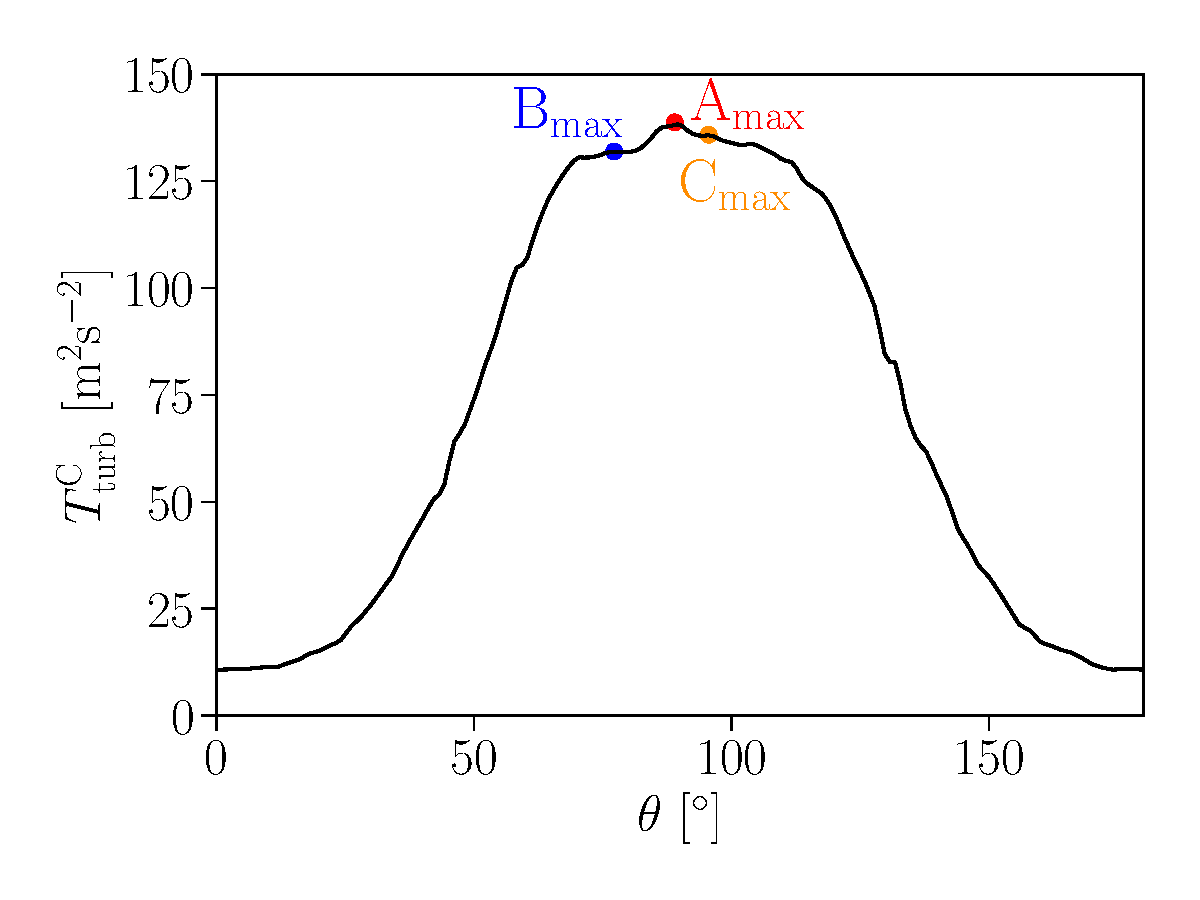
\includegraphics[width=1.19\textwidth]{Images/elip1maxpoints.pdf}
		\caption{Zobrazení bodů z tabulky \ref{tab:elip1max} nalezených v rámci maximalizace účelové funkce v úloze 5.1.}
		\label{fig:elip1maxbody}
	\end{subfigure}	
	\caption{Zobrazení různých bodů nalezených v rámci minimalizace a maximalizace účelové funkce v úloze 5.1 pomocí optimalizačních metod.}
	\label{fig:minmax elip1}
\end{figure}



\begin{figure}[H]
%	\centeringme
	\begin{subfigure}[b]{1.0\textwidth}
		\begin{center}
			\centering
			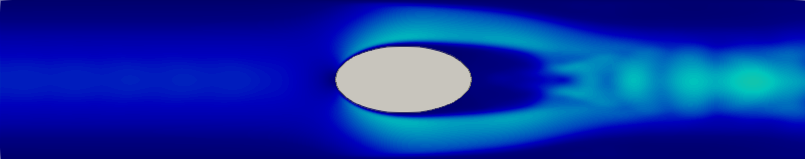
\includegraphics[width=0.8\textwidth, trim={0mm 0mm 0mm 0mm}]{Images/ellipse1_min_aaa.png}
			\vspace{2mm}
			\caption{Pole velikosti středních hodnot fluktuací pro $ \theta = 0^{\circ}$, tj. případ, kdy je $T^{\text{C}}_{\text{turb}} $ minimální.}
			\label{fig:elip1_0}
		\end{center}
		\vspace{2.8mm}
	\end{subfigure}
	\begin{subfigure}[b]{1.0\textwidth}
			\centering
			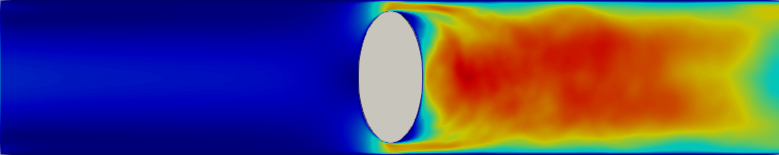
\includegraphics[width=0.8\textwidth, trim={0 0mm 0 0mm}]{Images/ellipse1_max_a.png}
			\vspace{1.8mm}
			\caption{Pole velikosti středních hodnot fluktuací pro $ \theta = 90^{\circ}$, tj. případ, kdy je $ T^{\text{C}}_{\text{turb}} $ maximální.}
			\label{fig:elip1_90}
	\end{subfigure}
	\begin{subfigure}[b]{1.0\textwidth}
		\centering
		\vspace{2.5mm}
		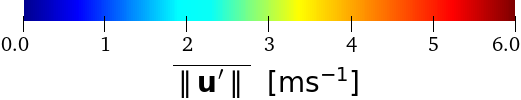
\includegraphics[width=0.45\textwidth, trim={0 0mm 0 0mm}]{Images/ellipse12_legenda.png}
	\end{subfigure}
	\caption{Porovnání velikosti středních hodnot fluktuací v úloze 5.1 pro případ s minimální turbulentní kinetickou energii a pro případ, kdy je turbulentní kinetická energie v oblasti C maximální.}
	\label{fig:1}
\end{figure}

Minimum nalezené metodou L-BFGS(A) souhlasilo s očekávaným výsledkem (zjištěným z interpolovaných hodnot) ve všech případech počátečních bodů. Minimum nalezené Nelderovou-Meadovou metodou pak ve dvou případech neodpovídalo skutečnému minimu, nicméně funkční hodnotou i polohou téměř se mu blížilo.

Maxima nalezená metodou L-BFGS(A) ve většině případů souhlasila s očekávaným výsledkem, v případech, kdy počáteční body byly krajními hodnotami množiny přípustných řešení, však nalezené maximum mělo pouze lokální charakter a nesouhlasilo tak se skutečným globálním maximem. Maxima nalezená Nelderovou-Meadovou metodou odpovídala globálnímu maximu ve všech případech.

Zejména u maximalizace můžeme pozorovat, že počet vyčíslení účelové funkce u metody L-BFGS(A) úzce souvisí s volbou počátečního bodu. V případech, kdy se počáteční bod blíží hledanému maximu, metoda konverguje při nižším počtu vyčíslení účelové funkce. U Nelderovy-Meadovy metody tuto závislost nepozorujeme. Můžeme vidět, že metoda L-BFGS(A) průměrně vyžaduje k nalezení řešení větší počet vyhodnocení účelové funkce, což je přirozeným důsledkem faktu, že v každé její iteraci je nutné numericky aproximovat gradient účelové funkce, což je realizováno pomocí schématu založeném na centrální diferenci.

\newpage

\subsection{Rotující elipsa s překážkou}
\begin{uloha}{Základní úloha rotující elipsy s překážkou}\label{ulo:2}
	\vspace{2mm}
	Nastavení úlohy:
	\begin{itemize}
		\item $ \Omega=(0 ; 2{,}5 \mathrm{~m}) \times(0 ; 0{,}5 \mathrm{~m})$
		\item $ \nu=10^{-3} \mathrm{~m}^{2} \mathrm{~s}^{-1}$
	\end{itemize} 
	Nastavení v rámci LBM:
	\begin{itemize}
		\item Na $ \overline{\hat{\Omega}} $ volíme počáteční podmínku podle sekce \ref{pocatecni podminka}.
		\item Na $ \partial \hat{\Omega}_{\mathrm{W}} $ volíme rychlost podle vztahu \eqref{eq:parabolic inflow} s $ U_m = 2{,}5 $ \si{m s^{-1}}.
		\item Na jednotlivých částech hranice $ \partial \hat{\Omega}$ předepisujeme momentovou okrajovou podmínku popsanou v sekci \ref{moment based bc}. Na hranici obtékaného objektu v oblasti B předepisujeme Bouzidiho interpolační podmínku rozebranou v sekci \ref{interpolation bc}. Na hranici překážky v oblasti A předepíšeme bounce-back okrajovou podmínku, viz sekce \ref{bounce-back}.
		\item Mřížku volíme jako $\overline{\hat{\Omega}} = N_{x} \times N_{y}$, $N_{x} = 1120, \, N_{y} = 224$,
		\item Kinematickou viskozitu v mřížkových jednotkách volíme $\nu^{L} = 10^{-3} $.
	\end{itemize}
	Použité objekty:
	\begin{itemize}
		\item V oblasti B předepsán objekt třídy \texttt{Ellipse} popsaný v sekci \ref{meshgenenator}. V oblasti A předepíšeme obdélník bez použití balíku \texttt{meshgenenator}.
	\end{itemize} 
	Použité optimalizační metody:
	\begin{itemize}
		\item Použijeme L-BFGS(A) a Nelderovu-Meadovu metodu (NM), obě metody jsou popsány v kapitole~\ref{optimalizace}.
	\end{itemize} 
\end{uloha}

\begin{figure}[H]
	\centering
	\vspace{8mm}
	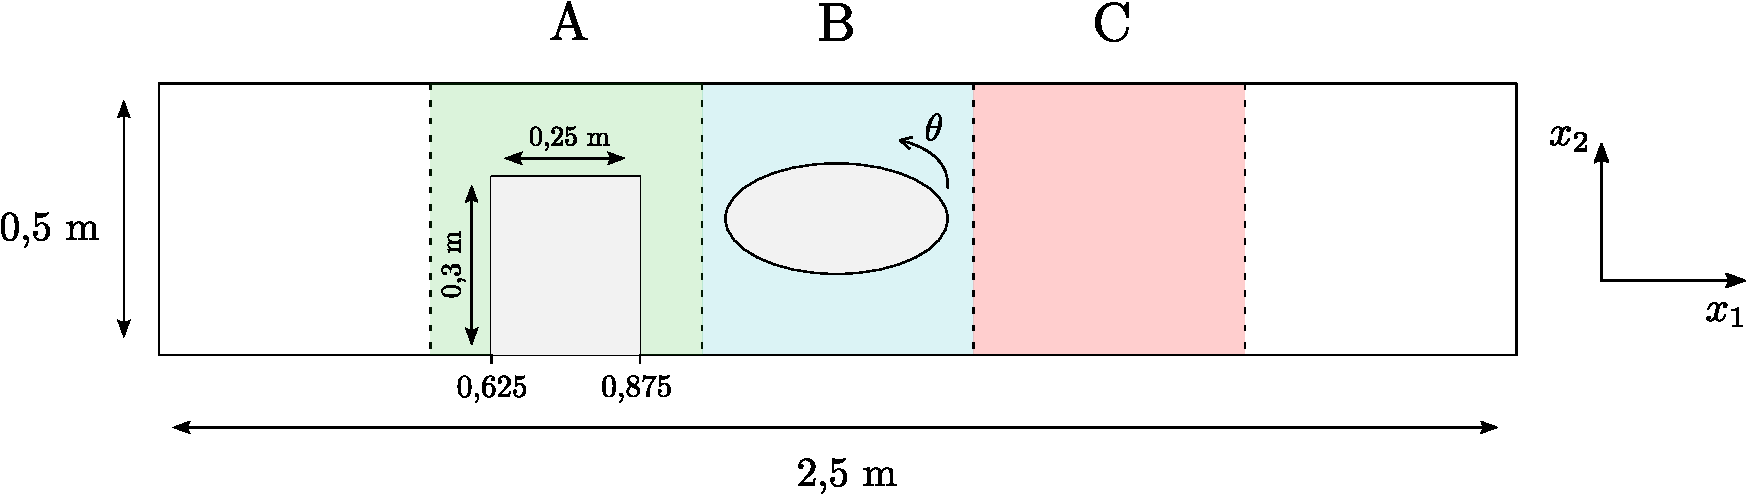
\includegraphics[width=1.0	\textwidth]{Images/elipsa2.pdf}
	\vspace{2mm}
	\caption{Schématické znázornění definice výpočetní oblasti v úloze 5.2.}
	\label{fig:elipsa 2}
	\vspace{1.8mm}
\end{figure}

V této úloze bude naším cílem zejména ověřit funkčnost optimalizačního rámce. Do oblasti B umístíme elipsu, která může rotovat kolem svého středu v rozsahu úhlu $0^\circ \leq \theta \leq 180^\circ$ tak, jako tomu bylo v úloze 5.1. V oblasti A pak dále umístíme obdélník tak, jak je znázorněno na obr. \ref{fig:elipsa 1}. Naším cílem opět bude maximalizovat, resp. minimalizovat $ T^{\text{C}}_{\text{turb}} (\theta) $ za již zmíněného předpokladu $0^\circ \leq \theta \leq 180^\circ$.

Analogicky jako v předchozí úloze definujeme ekvidistatní dělení $ k, k=0,1,\dots,180$ intervalu $0^\circ \leq \theta \leq 180^\circ$, v dělících bodech účelovou funkci pomocí numerických simulací vyčíslíme a lineárně tyto hodnoty interpolujeme. Interpolované hodnoty jsou společně s jejich maximem, resp. minimem zobrazeny na obr. \ref{fig:interpolovana elipsa 2}. Můžeme vidět, že maximum interpolované funkce je nabýváno při hodnotě $ \theta = 79^\circ $. Minimum se nachází v bodě $ \theta = 0^\circ $, resp. $ \theta = 180^\circ $. Můžeme pozorovat, že tvar interpolované funkce se z důvodu umístěné překážky v oblasti A změnil ve srovnání s úlohou 5.1. Interpolovaná funkce má nyní mimo globální maximum i další významná lokální maxima.

\begin{figure}[H]
	\centering
	\vspace{-2mm}
	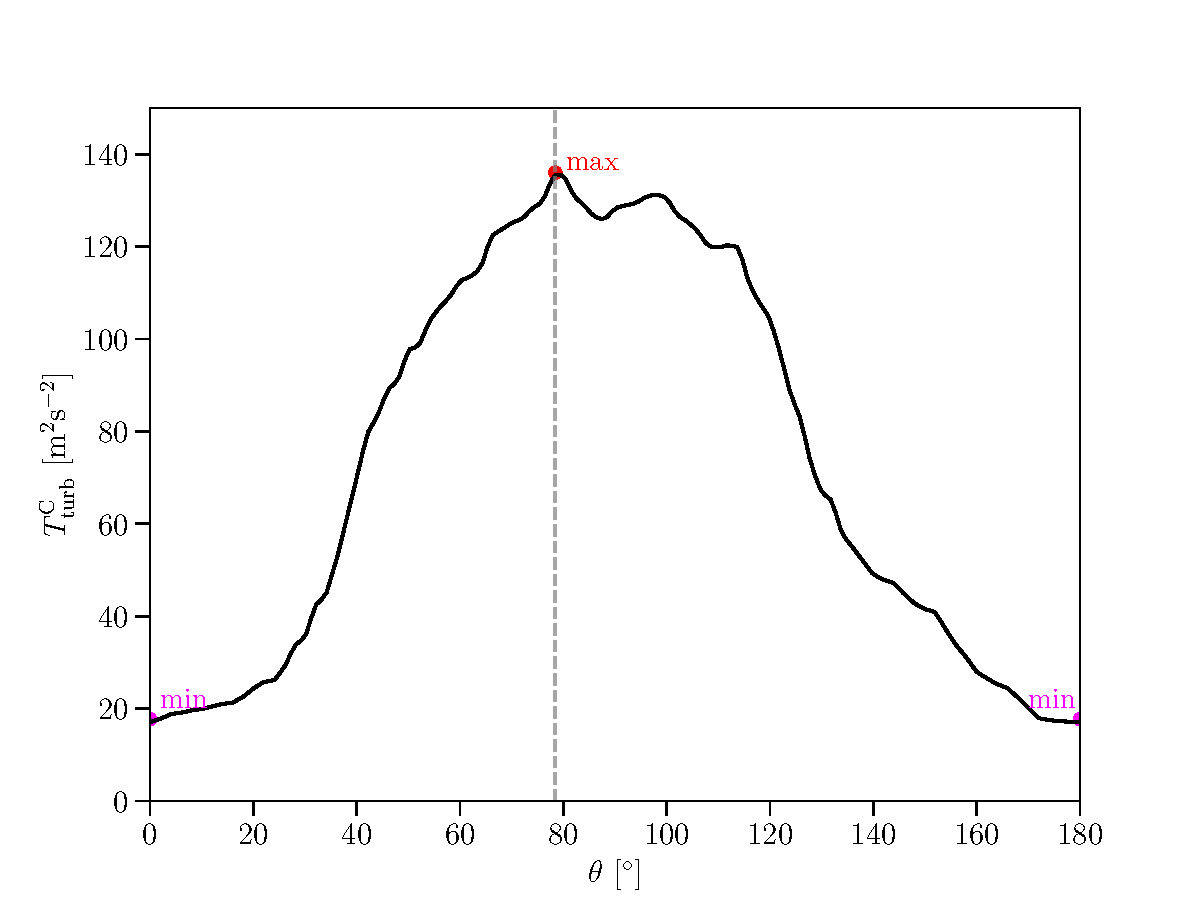
\includegraphics[width=0.82\textwidth]{Images/elip2interpolated.pdf}
	\vspace{2mm}
	\caption{Interpolované hodnoty pro úlohu 5.2 s vyznačeným maximem sloužící k následné jednodušší analýze výsledků.}
	\label{fig:interpolovana elipsa 2}
	\vspace{1.8mm}
\end{figure}

Pro minimalizaci a maximalizaci opět použijeme prvky množiny $ L $ definované pomocí \eqref{mnozina poc bodu} jako počáteční body. Výsledky minimalizace, resp. maximalizace jsou k nahlédnutí v tabulce \ref{tab:elip2min}, resp. v tabulce \ref{tab:elip2max}, kde používáme stejné značení jako v předchozí úloze. Body nalezené minimalizací, resp. maximalizací jsou znázorněny mezi interpolovanými hodnotami na obr. \ref{fig:elip2minbody}, resp. \ref{fig:elip2maxbody}. Na obr. \ref{fig:elip2_0}, resp. \ref{fig:elip2_79} je znázorněno pole středních hodnot fluktuací pro případ s minimální, resp. maximální turbulentní kinetickou energií.

\begin{minipage}{\textwidth}
	\hspace{-3mm}
	\begin{minipage}[b]{0.4\textwidth}
		\bgroup
		\setlength\tabcolsep{3mm}
		\def\arraystretch{1.7}%
		$$
		\begin{array}{ccc}
		\hline \text { Označení bodu } & \theta \, [^{\circ}] & T^{\text{C}}_{\text{turb}} (\theta) \, [\text{m}^{2} \text{s}^{-2}] \\
		\hline
		A_{\min} & 0{,}00 & 17{,}05 \\
		B_{\min} & 180{,}00 & 17{,}05 \\
		C_{\min} & 87{,}08 & 125{,}69 \\
		\hline
		\end{array}
		$$
		\egroup
	\end{minipage}%
	\begin{minipage}[b]{0.16\textwidth}
		\centering
		\hspace{-4mm}
	\end{minipage}%
	\begin{minipage}[b]{0.4\textwidth}
		\bgroup
		\setlength\tabcolsep{3mm}
		\def\arraystretch{1.7}%
		$$
		\begin{array}{ccc}
		\hline \text { Označení bodu } & \theta \, [^{\circ}] & T^{\text{C}}_{\text{turb}} (\theta) \, [\text{m}^{2} \text{s}^{-2}] \\
		\hline
		A_{\max} & 79{,}06 & 136{,}37 \\
		B_{\max} & 98{,}37 & 131{,}34 \\
		C_{\max} & 113{,}16 & 120{,}82 \\
		\hline
		\end{array}
		$$
		\egroup
	\end{minipage}
	\vspace{4mm}
	\hfill
\end{minipage}

\begin{minipage}{\textwidth}
	\begin{minipage}[b]{0.4\textwidth}
		\bgroup
		\setlength\tabcolsep{3mm}
		\def\arraystretch{1.5}%
		\begin{tabular}{|r|cc|cc|}
			\hline
			& \multicolumn{2}{c|}{L-BFGS(A)} & \multicolumn{2}{c|}{NM} \\ \hline
			\multicolumn{1}{|c|}{$\mathbf{x_0}$}& $\mathbf{x^\star}$ & $ \boldsymbol{\#f} $ & $\mathbf{x^\star}$ & $ \boldsymbol{\#f} $ \\ \hline
			$ 0^\circ $ 		&      A$_{\min}$           &     32     &    	A$_{\min}$   &  13 \\ 
			$ 30^\circ $ 		&      A$_{\min}$     		&     53     &    	A$_{\min}$   &  35 \\ 
			$ 60^\circ $ 		&      A$_{\min}$     		&     44     &    	A$_{\min}$   &  37 \\ 
			$ 90^\circ $ 		&      C$_{\min}$     		&     12     &    	B$_{\min}$   &  38 \\ 
			$ 120^\circ $ 		&      B$_{\min}$     		&     41     &      B$_{\min}$   &  31 \\ 
			$ 150^\circ $ 		&      B$_{\min}$     		&     25     &  	B$_{\min}$   &  41 \\
			$ 180^\circ $ 		&      B$_{\min}$     		&     68     &  	B$_{\min}$   &  18 \\ \hline
		\end{tabular}
		\vspace{2mm}
		\captionof{table}{Výsledky pro minimalizační úlohu s použitím metod L-BFGS(A) a~NM.}
		\label{tab:elip2min}
		\egroup
	\end{minipage}%
	\begin{minipage}[b]{0.15\textwidth}
		\centering
		\hspace{1mm}
	\end{minipage}%
	\begin{minipage}[b]{0.4\textwidth}
		\bgroup
		\setlength\tabcolsep{3mm}
		\def\arraystretch{1.5}%
		\begin{tabular}{|r|cc|cc|}
			\hline
			& \multicolumn{2}{c|}{L-BFGS(A)} & \multicolumn{2}{c|}{NM} \\ \hline
			\multicolumn{1}{|c|}{$\mathbf{x_0}$}& $\mathbf{x^\star}$ & $ \boldsymbol{\#f} $ & $\mathbf{x^\star}$ & $ \boldsymbol{\#f} $ \\ \hline
			$ 0^\circ $ 		&      A$_{\max}$           &     107    &    	A$_{\max}$   &  22 \\ 
			$ 30^\circ $ 		&      A$_{\max}$     		&     36     &    	A$_{\max}$   &  29 \\ 
			$ 60^\circ $ 		&      A$_{\max}$     		&     72     &    	A$_{\max}$   &  25 \\ 
			$ 90^\circ $ 		&      B$_{\max}$     		&     27     &    	A$_{\max}$   &  25 \\ 
			$ 120^\circ $ 		&      A$_{\max}$     		&     30     &      A$_{\max}$   &  28 \\ 
			$ 150^\circ $ 		&      C$_{\max}$     		&     45     &  	B$_{\max}$   &  7 \\
			$ 180^\circ $ 		&      A$_{\max}$     		&     106    &  	A$_{\max}$   &  26 \\ \hline
		\end{tabular}
		\vspace{2mm}
		\captionof{table}{Výsledky pro maximalizační úlohu s použitím metod L-BFGS(A) a~NM.}
		\label{tab:elip2max}
		\egroup
	\end{minipage}
	\hfill
\end{minipage}


\begin{figure}[H]
	\vspace{2mm}
	\begin{subfigure}[b]{0.45\textwidth}		
		\centering
		\hspace{-15mm}
		%		trim={<left> <lower> <right> <upper>}
		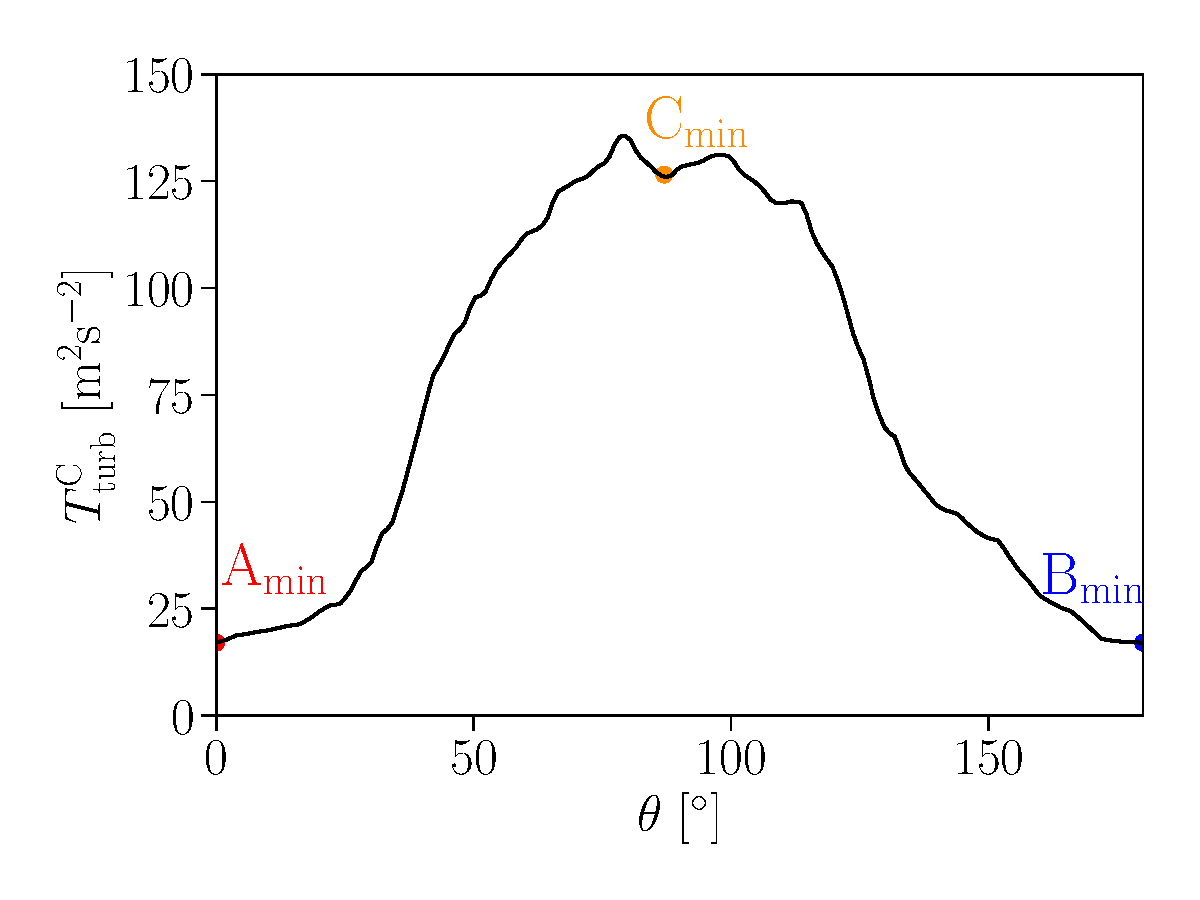
\includegraphics[width=1.19\textwidth]{Images/elip2minpoints.pdf}
		\caption{Zobrazení bodů z tabulky \ref{tab:elip2min} nalezených v rámci minimalizace účelové funkce v úloze 5.2.}
		\label{fig:elip2minbody}
	\end{subfigure}
	\begin{subfigure}[b]{0.12\textwidth}		
		\centering
		\hspace{-19mm}
	\end{subfigure}
	\begin{subfigure}[b]{0.45\textwidth}
		\centering
		\hspace{-15mm}
		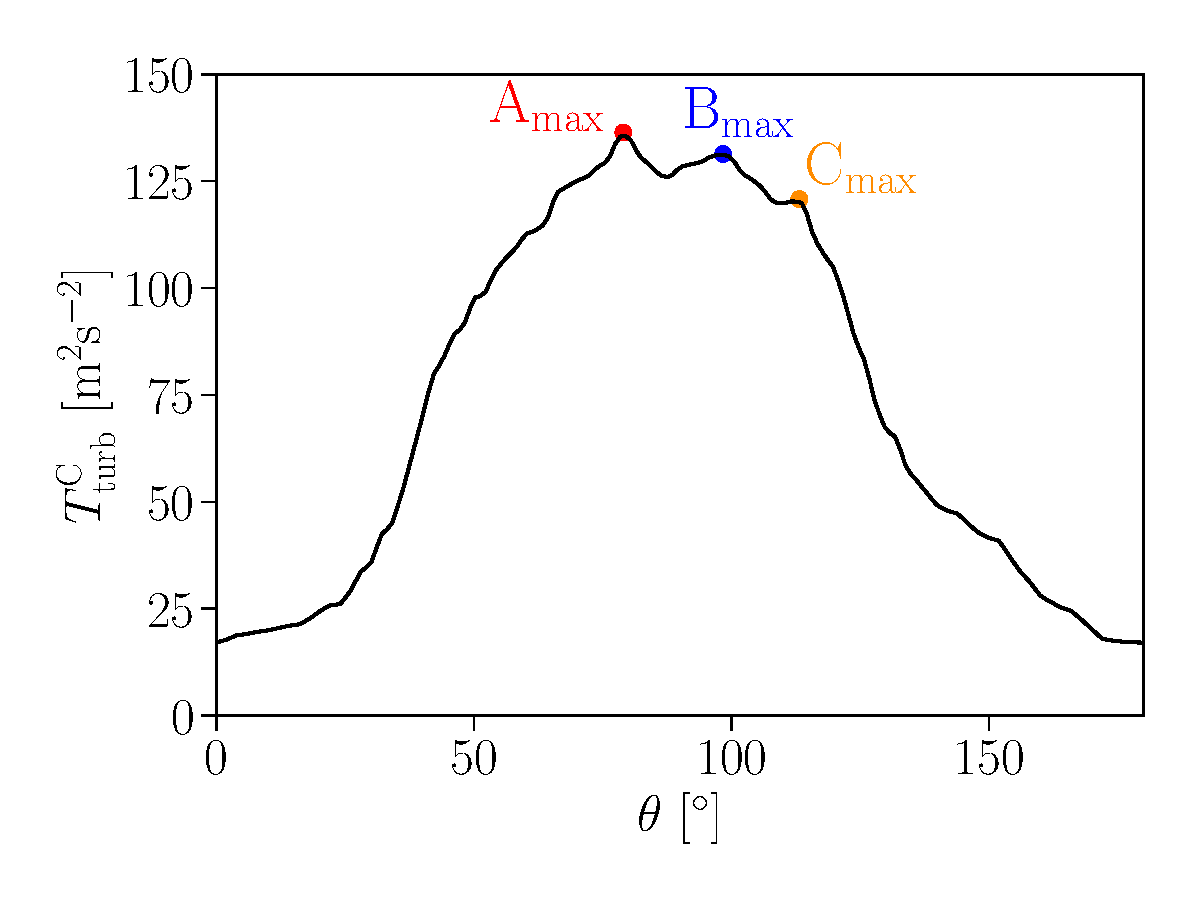
\includegraphics[width=1.19\textwidth]{Images/elip2maxpoints.pdf}
		\caption{Zobrazení bodů z tabulky \ref{tab:elip2max} nalezených v rámci maximalizace účelové funkce v úloze 5.2.}
		\label{fig:elip2maxbody}
	\end{subfigure}	
	\caption{Zobrazení různých bodů nalezených v rámci minimalizace a maximalizace účelové funkce v úloze 5.2 pomocí optimalizačních metod.}
	\label{fig:minmax elip2}
\end{figure}



\begin{figure}[H]
	\centering
	\begin{subfigure}[b]{1.0\textwidth}
		\begin{center}
			\centering
			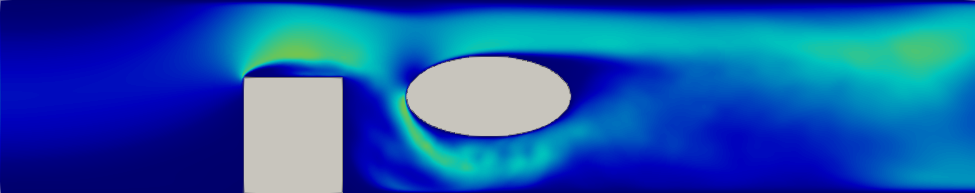
\includegraphics[width=0.8\textwidth, trim={0mm 0mm 0mm 0mm}]{Images/ellipse2_min_aa.png}
			\vspace{2mm}
			\caption{Pole střední velikosti fluktuací pro $ \theta = 0^{\circ}$.}
			\label{fig:elip2_0}
		\end{center}
		\vspace{2.8mm}
	\end{subfigure}
	\begin{subfigure}[b]{1.0\textwidth}
		\centering
		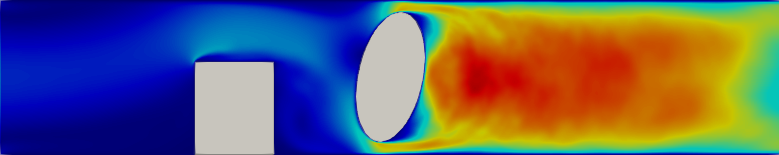
\includegraphics[width=0.8\textwidth, trim={0 0mm 0 0mm}]{Images/ellipse2_max_a.png}
		\vspace{1.8mm}
		\caption{Pole střední velikosti fluktuací pro $ \theta = 79{,}06^{\circ}$ - případ, kdy je $ T^{\text{C}}_{\text{turb}} $ maximální.}
		\label{fig:elip2_79}
	\end{subfigure}
	\begin{subfigure}[b]{1.0\textwidth}
		\centering
		\vspace{2.5mm}
		\includegraphics[width=0.5\textwidth, trim={0 0mm 0 0mm}]{Images/ellipse12_legenda.png}
	\end{subfigure}
	\caption{Porovnání velikosti středních hodnot fluktuací v úloze 5.2 pro případ s minimální turbulentní kinetickou energii a pro případ, kdy je turbulentní kinetická energie v oblasti C maximální.}
	\label{fig:2}
\end{figure}

Minimum nalezené metodou L-BFGS(A) souhlasilo s očekávaným výsledkem (zjištěným z interpolovaných hodnot) ve většině případů počátečních bodů. V jednom případě byl výsledek pouze lokálním minimem a zcela neodpovídal hledanému globálnímu minimu. Minimum nalezené Nelderovou-Meadovou metodou pak ve všech případech odpovídalo hledanému globálnímu minimu.

Maxima nalezená metodou L-BFGS(A) opět ve většině případů odpovídala očekávanému výsledku, ve dvou případech však výsledek odpovídal lokálním maximům rozdílným od globálního maxima. Maxima nalezená Nelderovou-Meadovou odpovídala globálnímu maximu až na jeden případ, kdy bylo nalezeno rozdílné lokální maximum.

Jako tomu bylo v úloze 5.1, i zde můžeme pozorovat, že metoda L-BFGS(A) průměrně vyžaduje k nalezení řešení větší počet vyhodnocení účelové funkce, přičemž tento počet je úzce spjat s volbou počátečního bodu. U Nelderovy-Meadovy metody jsme toto nepozorovali.

\subsection{Shrnutí výsledků úloh s jedním parametrem}
V rámci úloh 5.1 a 5.2 se podařilo úspěšně prokázat funkčnost navrženého optimalizačního rámce.  Díky interpolovaným hodnotám získaným pomocí vyčíslení účelové funkce v dostatečně mnoho bodech diskretizujících množinu přípustných řešení jsme mohli ověřit správnost výsledků získaných pomocí optimalizačních metod. Tyto výsledky v uspokojivé míře odpovídaly výsledkům očekávaným.

Již pro úlohu s jedním optimalizačním parametrem bylo možné pozorovat, že pro některé volby počátečních bodů může být metoda L-BFGS(A) časově mnohem náročnějí, než Nelderova-Meadova metoda. Nelderova-Meadova metoda byla dále také v průměru úspěšnější v hledání správného řešení. Na základě výše zmíněného lze usuzovat, že Nelderova-Meadova metoda představuje lepší volbu v uvažovaném optimalizačním rámci.


\newpage
\section{Úloha s dvěma optimalizačními parametry}
\begin{uloha}{Rotující Cassiniho ovál s konstantním obsahem}\label{ulo:3}
	\vspace{2mm}
	Nastavení úlohy:
	\begin{itemize}
		\item $ \Omega=(0 ; 2{,}5 \mathrm{~m}) \times(0 ; 0{,}5 \mathrm{~m})$
		\item $ \nu=10^{-3} \mathrm{~m}^{2} \mathrm{~s}^{-1}$
	\end{itemize} 
	Nastavení v rámci LBM:
	\begin{itemize}
		\item Na $ \overline{\hat{\Omega}} $ volíme počáteční podmínku podle sekce \ref{pocatecni podminka}.
		\item Na $ \partial \hat{\Omega}_{\mathrm{W}} $ volíme rychlost podle vztahu \eqref{eq:parabolic inflow} s $ U_m = 2{,}5 $ \si{m s^{-1}}.
		\item Na jednotlivých částech hranice $ \partial \hat{\Omega}$ předepisujeme momentovou okrajovou podmínku popsanou v sekci \ref{moment based bc}. Na hranici obtékaného objektu v oblasti B předepisujeme Bouzidiho interpolační podmínku rozebranou v sekci \ref{interpolation bc}.
		\item Mřížku volíme jako $\overline{\hat{\Omega}} = N_{x} \times N_{y}$, $N_{x} = 1120, \, N_{y} = 224$,
		\item Kinematickou viskozitu v mřížkových jednotkách volíme $\nu^{L} = 10^{-3} $.
	\end{itemize}
	Použité objekty:
	\begin{itemize}
		\item V oblasti B předepsán objekt třídy \texttt{CassiniOval} popsaný v sekci \ref{meshgenenator}.
	\end{itemize} 
	Použité optimalizační metody:
	\begin{itemize}
		\item Použijeme L-BFGS(A) a Nelderovu-Meadovu metodu (NM), obě metody jsou popsány v kapitole~\ref{optimalizace}.
	\end{itemize} 
\end{uloha}

\begin{figure}[H]
	\centering
	\vspace{8mm}
	\includegraphics[width=1.0	\textwidth]{Images/cassini.pdf}
	\vspace{2mm}
	\caption{Schématické znázornění definice výpočetní oblasti v úloze 5.1.}
	\label{fig:cassini oblast}
	\vspace{1.8mm}
\end{figure}

\newpage

V této úloze bude naším cílem formulovat a řešit úlohu s netriviálním tvarem účelové funkce. Výpočetní oblast opět rozdělíme na pět stejných částí se stejným značením jako tomu bylo v předchozích úlohách. Do oblasti B umístíme Cassiniho ovál popsaný rovnicí
\begin{equation}
\left[(x-x_s)^2 + (y-y_s)^2 + a^2 \right] ^2 - 4a^2(x-x_s)^2 = b^4,
\end{equation}
kde $ a $ a $ b $ jsou parametry a dále $\, x_s = 1{,}25$ a $ y_s = 0{,}25 $, přičemž všechny uvedené parametry mají rozměr~\si{[m]}. Nastavení úlohy je schematicky znázorněno na obr.~\ref{fig:cassini oblast}. Prvním stupněm volnosti bude podobně jako v předchozích úlohách možnost rotace oválu kolem svého středu. Umožníme rotaci v rozsahu úhlu $45^\circ \leq \theta \leq 125^\circ$. Dále připustíme různé hodnoty parametru $ a $, konkrétně požadujeme \mbox{$0{,}08 \text{ m} \leq a \leq 0{,}13 \text{ m}$}, čímž jsou určeny další nerovnostní vazby. Parametr $ a $ a úhel $ \theta $ budou představovat optimalizační parametry. Pro optimalizaci využijeme metodu L-BGFS(A) a Nelderovu-Meadovu metodu.

Pro jednoznačné určení parametru $ b $ na základě hodnoty $ a $ budeme požadovat, aby měl ovál stále stejný obsah - konkrétně požadujeme zachování hodnoty obsahu $ S = 0{,}0545 $ \si{m^2}. Obsah Cassiniho oválu lze za zmíněných předpokladů vyjádřit rovnicí \cite{Cassini}
\begin{equation}\label{eq:cassini area}
S = a^2 + b^2 E\left(\frac{a^2}{b^2}\right),
\end{equation}
kde $ E(x) $ značí eliptický integrál druhého druhu. V každé iteraci optimalizačního algoritmu tedy před generováním geometrie pro aktuální sadu hodnot optimalizačních parametrů numericky vyřešíme rovnici \ref{eq:cassini area} pro neznámou hodnotu~$ b $ pomocí Powellovy hybridní metody implementované ve volně dostupné knihovně SciPy.

Označíme turbulentní kinetickou energii v oblasti C závislou na úhlu $ \theta $ a parametru $ a $ jako $ T^{\text{C}}_{\text{turb}} (a, \theta) $. Cílem bude maximalizovat $ T^{\text{C}}_{\text{turb}} (a, \theta) $ za zmíněných předpokladů nerovnostních vazeb \mbox{$45^\circ \leq \theta \leq 120^\circ$} a \mbox{$0{,}08 \text{ m} \leq a \leq 0{,}13 \text{ m}$} při zachování obsahu $ S = 0{,}0545 $ \si{m^2}.

Zavedeme množinu bodů
\begin{equation}\label{eq:mnozina M}
	M = \big\{ \, (0{,}08 + 0{,}002i; \, 45 + 3j) \: \big| \: i,j = 0, 1, \dots, 25 \,  \big\},
\end{equation}
která diskretizuje prostor optimalizačních parametrů. V bodech množiny \ref{eq:mnozina M} vypočteme pomocí numerických simulací hodnoty účelové funkce $ T^{\text{C}}_{\text{turb}} (a, \theta) $, které následně lineárně interpolujeme. Interpolované hodnoty jsou společně s jejich maximem, které je nabýváno při hodnotách $ a = 0{,}126 $ m, $ \theta = 96^\circ $, zobrazeny na obr. \ref{fig:interpolovany cassini}. Tyto hodnoty využijeme k následné snadnější analýze výsledků optimalizačních metod. Zdůrazněme, že v rámci optimalizace interpolované hodnoty nevyužíváme.


\begin{figure}[H]
	\centering
	\vspace{-15mm}
	\includegraphics[width=0.8\textwidth]{Images/cassini2Dinterpolated.png}
	\caption{Interpolované hodnoty pro úlohu 5.3 s vyznačeným maximem sloužící k následné jednodušší analýze výsledků.}
	\label{fig:interpolovany cassini}
\end{figure}

Použité počáteční body $\mathbf{x_0}$ a jejich označení je uvedeno v tabulce \ref{tab:pocatecni body}:

\begin{center}
	
\bgroup
\setlength\tabcolsep{3mm}
\def\arraystretch{1.6}%
\begin{tabular}{ccc}
	\hline 
	Označení $\mathbf{x_0}$  & $ a \, [\text{m}]$ & $ \theta \, [^{\circ}] $\\
	\hline
	A$_0$ & 0{,}097 & $ 75 $ \\
	B$_0$ & 0{,}084 & $ 115 $ \\
	C$_0$ & 0{,}113 & $ 102 $\\
	\hline

\end{tabular}
\vspace{1mm}
\captionof{table}{Počáteční body použité v úloze 5.3 a jejich označení.}
\label{tab:pocatecni body}
\egroup
\end{center}

Výsledné body nalezené pomocí optimalizačních metod budeme značit vždy písmenem příslušným použitému počátečnímu bodu, hvězdičkou v horním indexu a zkráceným názvem metody v dolním indexu. Výsledky získané pro jednotlivé počáteční body jsou k nahlédnutí v tabulce \ref{tab:vysledky cassini}.
\vspace{3mm}
\begin{center}
	\bgroup
\setlength\tabcolsep{3mm}
\def\arraystretch{1.7}%
\begin{tabular}{|r|cccc|cccc|}
	\hline
	& \multicolumn{4}{c|}{L-BFGS(A)} & \multicolumn{4}{c|}{NM} \\ \hline
	\multicolumn{1}{|c|}{$\mathbf{x_0}$}& $\mathbf{x^\star}$ & $ a \, [\text{m}] $ & $ \theta \, [^{\circ}]$ & $ T^{\text{C}}_{\text{turb}} (a, \theta) \, [\text{m}^{2} \text{s}^{-2}]$ & $\mathbf{x^\star}$ & $ a \, [\text{m}] $ & $ \theta \, [^{\circ}]$ & $ T^{\text{C}}_{\text{turb}} (a, \theta) \, [\text{m}^{2} \text{s}^{-2}]$  \\ \hline
	A$_0$ 		&      A$^{\star}_{\text{L-BFGS}}$          &     0,122 &     88,27 &     125{,}58    &    	A$^{\star}_{\text{NM}}$ &     0,128 &     77,66   &  131,76 \\ 
	B$_0$ 		&      B$^{\star}_{\text{L-BFGS}}$     		&     0,083 &     113,5 &     90,68    &    	B$^{\star}_{\text{NM}}$    &     0,126 &     95,73   &  135,51 \\ 
	C$_0$ 		&      C$^{\star}_{\text{L-BFGS}}$     		&     0.128 &     77,66 &     131,76    &    	C$^{\star}_{\text{NM}}$   &     0,127 &     90,06   &  128,25 \\  
	\hline
\end{tabular}
\vspace{2mm}
\captionof{table}{Výsledky pro maximalizační úlohu s použitím metod L-BFGS(A) a~NM}
\label{tab:vysledky cassini}
\egroup
\end{center}

%\begin{figure}[H]
%	\vspace{2mm}
%	\begin{subfigure}[b]{0.61\textwidth}		
%		\hspace{-19mm}
%		\centering
%		%		trim={<left> <lower> <right> <upper>}
%		\includegraphics[width=1.12\textwidth]{Images/1full.png}
%	\end{subfigure}
%	\begin{subfigure}[b]{0.001\textwidth}
%		\centering
%		\hspace{1mm}
%	\end{subfigure}	
%	\begin{subfigure}[b]{0.38\textwidth}
%		\bgroup
%		\setlength\tabcolsep{1.5mm}
%		\def\arraystretch{1.2}%
%		$$
%		\begin{array}{|c|ccc|}
%		\hline \text { Metoda } & \theta & a & T^{\text{C}}_{\text{turb}} (\theta) \\
%		\hline
%		\text { L-BFGS(A) } & 79{,}00 & 136{,}37 & 136{,}37\\
%		\text { NM } & 98{,}37 & 131{,}34 & 136{,}37\\
%		\hline
%		\end{array}
%		$$
%		\egroup
%		\centering
%		\vspace{-2mm}
%		\includegraphics[width=1.1\textwidth, trim={12mm 0 0 5mm}]{Images/1.pdf}
%		\vspace{-15mm}
%	\end{subfigure}	
%    \vspace{2mm}
%	\caption{Zobrazení různých bodů nalezených v rámci minimalizace a maximalizace účelové funkce v úloze 5.2 pomocí optimalizačních metod.}
%\end{figure}

Pro každý z počátečních bodů dále zobrazíme výsledky optimalizačních metod mezi interpolovanými hodnotami. Pro počáteční body také porovnáme u obou metod rychlost konvergence k výsledku, tj. postupné zlepšování odhadu řešení v závislosti na počtu vyhodnocení účelové funkce. Zmíněné výsledky jsou k nahlédnutí na obr. \ref{fig:vysledky cassini}.

\begin{figure}[H]
	\begin{subfigure}[b]{1.0\textwidth}		
	\begin{subfigure}[b]{0.61\textwidth}		
		\hspace{-19mm}
		\centering
		%		trim={<left> <lower> <right> <upper>}
		\includegraphics[width=1.06\textwidth, trim={0mm 4mm 0 6mm}]{Images/1full.png}
		\vspace{3mm}
	\end{subfigure}
	\begin{subfigure}[b]{0.001\textwidth}
		\centering
		\hspace{1mm}
	\end{subfigure}	
	\begin{subfigure}[b]{0.38\textwidth}
		\centering
		\vspace{-2mm}
		\includegraphics[width=1.1\textwidth, trim={12mm 0 0 0mm}]{Images/1.pdf}
	\end{subfigure}	
	\caption{Výsledné nalezené body a graf rychlosti konvergence metod k řešení pro počáteční bod A$_0$. V pravé části obrázku je znázorněn odhad optimálního řešení v závislosti na počtu vyčíslení účelové funkce pomocí numerické simulace, který je označen jako $ \# f $. \vspace{6mm}}
	\end{subfigure}

	\begin{subfigure}[b]{1.0\textwidth}		
	\begin{subfigure}[b]{0.61\textwidth}		
		\hspace{-19mm}
		\centering
		%		trim={<left> <lower> <right> <upper>}
		\includegraphics[width=1.06\textwidth, trim={0mm 4mm 0 5mm}]{Images/2full.png}
		\vspace{3mm}
	\end{subfigure}
	\begin{subfigure}[b]{0.001\textwidth}
		\centering
		\hspace{1mm}
	\end{subfigure}	
	\begin{subfigure}[b]{0.38\textwidth}
		\centering
		\vspace{-2mm}
		\includegraphics[width=1.1\textwidth, trim={12mm 0 0 0mm}]{Images/2.pdf}
	\end{subfigure}	
	\caption{Výsledné nalezené body a graf rychlosti konvergence metod k řešení pro počáteční bod B$_0$.  V pravé části obrázku je znázorněn odhad optimálního řešení v závislosti na počtu vyčíslení účelové funkce pomocí numerické simulace, který je označen jako $ \# f $. \vspace{6mm}}
	\end{subfigure}
\end{figure}
\begin{figure}[h]
	\vspace{-10mm}
	\ContinuedFloat 
	\begin{subfigure}[b]{1.0\textwidth}		
	\begin{subfigure}[b]{0.61\textwidth}		
		\hspace{-19mm}
		\centering
		%		trim={<left> <lower> <right> <upper>}
		\includegraphics[width=1.06\textwidth, trim={0mm 4mm 0 15mm}]{Images/3full.png}
		\vspace{3mm}
	\end{subfigure}
	\begin{subfigure}[b]{0.001\textwidth}
		\centering
		\hspace{1mm}
	\end{subfigure}	
	\begin{subfigure}[b]{0.38\textwidth}
		\vspace{-10mm}
		\centering
		\vspace{-2mm}
		\includegraphics[width=1.1\textwidth, trim={12mm 0 0 0mm}]{Images/3.pdf}
	\end{subfigure}	
	\caption{Výsledné nalezené body a graf rychlosti konvergence metod k řešení pro počáteční bod C$_0$.  V pravé části obrázku je znázorněn odhad optimálního řešení v závislosti na počtu vyčíslení účelové funkce pomocí numerické simulace, který je označen jako $ \# f $. \vspace{2mm}}
	\end{subfigure}
	\caption{Zobrazení bodů nalezených v rámci maximalizace účelové funkce v úloze 5.3 pomocí optimalizačních metod a graf aktuálního odhadovaného řešení v závislosti na $ \# f $, tj. na počtu vyčíslení účelové funkce pomocí numerické simulace, pro jednotlivé počáteční body.}
	\label{fig:vysledky cassini}
\end{figure}

\newpage

Pro srovnání s výsledkem maximalizace v úloze 5.1 uvádíme na obr. \ref{fig:paraview cassini} pole středních hodnot fluktuací pro případ s maximální turbulentní kinetickou energií.

\begin{figure}[H]
	\vspace{3mm}
	\centering
	\includegraphics[width=0.71	\textwidth]{Images/cassini_max.png}

	\caption{Pole střední velikosti fluktuací pro $a = 0{,}126$ m a $ \theta = 95{,}73^{\circ}$ - případ, kdy je $ T^{\text{C}}_{ \text{turb}} $ maximální.}
	\label{fig:paraview cassini}
\end{figure}

\subsection{Shrnutí výsledků úlohy s dvěma parametry}
V rámci úlohy 5.3 jsme demonstrovali možnost použití navrženého optimalizačního rámce na úlohy s komplexnější formulací. Získané výsledky pomocí optimalizace jsme porovnali s interpolovanými hodnotami nahrazujícími účelovou funkci, díky čemuž jsme mohli ověřit jejich správnost. Bylo možné pozorovat, že výsledky nalezené Nelderovou-Meadovou metodou odpovídaly správnému řešení nebo se mu blížily. K nalzení řešení navíc Nelderova-Meadova metoda potřebovala vždy méněkrát vyčíslit účelovou funkci, což je pro nás jedním ze stěžejních faktorů. Lze tedy opět usoudit, že Nelderova-Meadova metoda představuje lepší volbu v navrženém optimalizačním rámci.
\newpage
\section{Úloha s třemi optimalizačními parametry}

\begin{uloha}{Zjednodušený model totálního kavopulmonárního napojení (TCPC)}\label{ulo:4}
	\vspace{2mm}
	Nastavení úlohy:
	\begin{itemize}
		\item $ \Omega=(0 ; L_1) \times(0 ; L_2)$, kde $ L_1 = 4 \mathrm{~m}$, $ L_2 = 2\mathrm{~m} $
		\item $ \nu=10^{-3} \mathrm{~m}^{2} \mathrm{~s}^{-1}$
	\end{itemize} 
	Nastavení v rámci LBM:
	\begin{itemize}
		\item Na $ \overline{\hat{\Omega}} $ volíme počáteční podmínku podle sekce \ref{pocatecni podminka}.
		\item Na $ \partial \hat{\Omega}_{} $ zavedeme části $ \Gamma^{\mathrm{W}}_{\mathrm{out}}, \Gamma^{\mathrm{E}}_{\mathrm{out}}, \Gamma^{\mathrm{S}}_{\mathrm{in}}, \Gamma^{\mathrm{N}}_{\mathrm{in}} $ podle obr. \ref{fig:tcpc oblast}.
		\item Na $ \Gamma^{\mathrm{S}}_{\mathrm{in}} $ volíme parabolický profil rychlosti s maximální rychlostí $ 1{,}8 $ \si{m s^{-1}}. Na $ \Gamma^{\mathrm{N}}_{\mathrm{in}} $ volíme parabolický profil rychlosti s maximální rychlostí $ 1{,}5 $ \si{m s^{-1}}.
		\item Na $ \Gamma^{\mathrm{W}}_{\mathrm{out}}, \Gamma^{\mathrm{E}}_{\mathrm{out}} $ předepisujeme rovnovážnou okrajovou podmínku popsanou v sekci \ref{equilibrium bc}. Na hranici obtékaných objektů předepisujeme Bouzidiho interpolační podmínku rozebranou v sekci \ref{interpolation bc}. 
		
		\item Mřížku volíme jako $\overline{\hat{\Omega}} = N_{x} \times N_{y}$, $N_{x} = 448, \, N_{y} = 224$,
		\item Kinematickou viskozitu v mřížkových jednotkách volíme $\nu^{L} = 10^{-3} $.
	\end{itemize}
	Použité objekty:
	\begin{itemize}
		\item V oblasti předepíšeme čtyři objekty třídy \texttt{FunctionCurve}, která je popsána v sekci \ref{meshgenenator}. Jako funkce volíme hyperboly.
	\end{itemize} 
	Použité optimalizační metody:
	\begin{itemize}
		\item Použijeme Nelderovu-Meadovu metodu popsanou v kapitole~\ref{optimalizace}.
	\end{itemize} 
\end{uloha}
\vspace{-1mm}
\begin{figure}[H]
	\centering
	\includegraphics[width=0.61	\textwidth]{Images/krizovatka-obecna.pdf}
%	\vspace{2mm}
	\caption{Schématické znázornění definované výpočetní oblasti s jejími rozměry a částí její hranice označenými $ \Gamma^{\mathrm{W}}_{\mathrm{out}}, \Gamma^{\mathrm{E}}_{\mathrm{out}}, \Gamma^{\mathrm{S}}_{\mathrm{in}}, \Gamma^{\mathrm{N}}_{\mathrm{in}} $.}
	\label{fig:tcpc oblast}
	\vspace{1.8mm}
\end{figure}

Cílem této úlohy je řešit zjednodušený model inspirovaný geometrií TCPC ve 2D, která je znázorněna na obr. \ref{fig:tcpc}. S rozměry oblasti $ \Omega=(0 ; 4 \mathrm{~m}) \times(0 ; 2\mathrm{~m})$ a kinematickou viskozitou \mbox{$ \nu=10^{-3} \mathrm{~m}^{2} \mathrm{~s}^{-1}$} zjevně nastavení řešené úlohy neodpovídá reálným hodnotám fyzikálních parametrů úlohy TCPC. Použitím zákona podobnosti pro dynamiku tekutin (rovnost Reynoldsova čísla v porovnávaných systémech) lze však ukázat, že použité nastavení úlohy je ekvivalentní systému s rozměry a viskozitou řádově odpovídajícími reálné úloze TCPC. Reálná šířka konduitu se typicky pohybuje okolo 2 cm, kinematická viskozita krve je $ 4 \cdot 10^{-6} $ \si{m^2.s^{-1}} \cite{Rijnberg2018}. Podotkněme, že cílem této úlohy však není vytvořit přesný model systému s totálním kavopulmonárním napojením, ale spíše otestovat optimalizační rámec na úloze připomínající geometrii TCPC.

Při návrhu optimalizační úlohy byly zohledněny faktory, které lze kontrolovat v rámci geometrie TCPC a u kterých bylo prokázáno, že mají pozitivní vliv na minimalizaci ztrát energie v systému \cite{Rijnberg2018}. Možné modifikace napojení, které snižují ztráty energie a zajišťují lepší funkčnost systému jsou zobrazeny na obr. \ref{fig:tcpc modifikace}. Byla prokázána vhodnost takto modifikovaných geometrií, které lze dále analyzovat např. pomocí numerických simulací \cite{Rijnberg2018, Porfiryev2020, Ensley1999}.


\begin{figure}[H]
	\centering
	\vspace{8mm}
	\includegraphics[width=0.75	\textwidth]{Images/energyloss.pdf}
	\vspace{9mm}
	\caption{Schématické znázornění možných modifikací, kterými lze zmenšit ztráty energie v systému s TCPC a díky nimž lze zmenšit např. silové působení proudění na stěny v oblasti \cite{Rijnberg2018}. Schéma je převzato z \cite{Rijnberg2018}, přičemž popisky jsou přeloženy do češtiny.}
	\label{fig:tcpc modifikace}
	\vspace{1.8mm}
\end{figure}


Cílem této úlohy je sledovat, zda výsledek optimalizační úlohy v systému s uvažovanou geometrií TCPC se stupni volnosti umožňujícími rozšíření a posunutí dolního kanálu (body a) a d) na obr.~\ref{fig:tcpc modifikace}) bude odpovídat výsledkům z dostupné literatury a zda bude mít systém tendenci dospět k některým z výše pospsaných modifikací. Pro generování geometrie zvolíme objekty třídy \texttt{FunctionCurve}, která je popsána v sekci \ref{meshgenenator}. Budeme volit čtyři hyperboly S$_1$, S$_2$, S$_3$ a S$_4$ v~následujícím tvaru:

\begin{align}\label{eq:hyperboly}
\begin{split}
\mathrm{S}_1 &: \hspace{7mm} y = -\frac{1}{k_2[x-(o_2 + 0{,}25 + l_2)]} + h - 0{,}25 \, , \hspace{3mm}x > o_2 + 0{,}25 + l_2,\\[6pt]
\mathrm{S}_2 &: \hspace{7mm} y = \frac{1}{k_1[x-(o_1 + 0{,}25)]} + h + 0{,}25 \, , \hspace{3mm}x > o_1 + 0{,}25,\\[6pt]
\mathrm{S}_3 &: \hspace{7mm} y = -\frac{1}{k_1[x-(o_1 - 0{,}25)]} + h + 0{,}25 \, , \hspace{3mm}x < o_1 - 0{,}25,\\[6pt]
\mathrm{S}_4 &: \hspace{7mm} y = \frac{1}{k_2[x-(o_2 - 0{,}25 - l_2)]} + h - 0{,}25 \, , \hspace{3mm}x < o_2 + 0{,}25 + l_2,\\[15pt]
\end{split}
\end{align}
kde $ h = 1$ m, $ o_1 = 2{,}5$ m, $ k_1 = 250$, a $ o_2 \, \si{[m]}¨, k_2 \, \si{[-]}$ a $ l_2 \, \si{[m]}$ jsou konstanty dále použité jako optimalizační parametry. Parametr $ o_2 $ odpovídá posunutí dolního kanálu, $ k_2 $ odpovídá rošíření části dolního kanálu, kde ústí do vodorovného kanálu, a parametr $ l_2 $ odpovídá modifikaci šířky dolního kanálu. Pro zmíněné parametry budeme předpokládat následující nerovnostní vazby:

\begin{subequations}\label{eq:tcpc vazby}
	\begin{eqnarray}
	1{,}25 \text{ m} &\leq& o_2 \hspace{1.5mm}\leq  \hspace{1.5mm}2{,}75 \text{ m} \, ,\\[3pt]
	-0{,}05 \text{ m} &\leq& l_2 \hspace{2.5mm}\leq \hspace{1.5mm}0{,}05 \text{ m} \, ,\\[3pt]
	50 &\leq& k_2 \hspace{2mm}\leq \hspace{1.5mm}200 \, .
	\end{eqnarray}
\end{subequations}
Dále zavedeme podoblast A $ = (0{,}50~\text{m}; 3{,}50~\text{m}) \times (0{,}36~\text{m}; 1{,}64~\text{m})$, na které budeme vyhodnocovat účelové funkce. Schématické znázornění definice geometrie, optimalizačních parametrů a podblasti A je k nahlédnutí na obr. \ref{fig:tcpc oblast 2}.
\begin{figure}[H]
	\centering
	\vspace{10mm}
	\includegraphics[width=0.66	\textwidth]{Images/krizovatka.pdf}
	\vspace{2mm}
	\caption{Význam optimalizačních parametrů a definice oblasti A, v níž je optimalizována účelová funkce.}
	\label{fig:tcpc oblast 2}
	\vspace{1.8mm}
\end{figure}
Označíme $ \dot{\gamma} ^{A}_{\text{wall}}(o_2, k_2, l_2) $ smykovou rychlost (definovanou jako \ref{eq:dot gamma}) podél stěn v oblasti A. Dále označíme $ T^{\text{A}}_{\text{turb}} (o_2, k_2, l_2) $ turbulentní kinetickou energii v oblasti A. Tyto dvě účelové funkce budeme postupně v rámci této úlohy minimalizovat pomocí Nelderovy-Meadovy metody s počátečním bodem splňujícím $ o_2 = 2{,}5 $ m, $ k_2 = 200 $ a $ l_2 = 0 $  m, přičemž v rámci optimalizace předpokládáme nerovnostní vazby~\ref{eq:tcpc vazby}. Počáteční bod odpovídá situaci, kdy jsou oba kanály stejně široké a bez posunu, přičemž dolní kanál je mírně rozšířen ve svém ústí.

Výsledky pro minimalizaci $ \dot{\gamma} ^{A}_{\text{wall}}(o_2, k_2, l_2) $ jsou k nahlédnutí na obr. \ref{fig:tcpc gamma veloc}, \ref{fig:tcpc gamma fluc} a \ref{fig:tcpc dotgamma shear rate}. Na obr. \ref{fig:tcpc gamma veloc} je znázorněno pole střední velikosti rychlosti v oblasti A, na obr. \ref{fig:tcpc gamma fluc} je znázorněno pole střední velikosti fluktuací v oblasti A a na obr. \ref{fig:tcpc dotgamma shear rate} je znázorněna střední smyková rychlost podél stěn v oblasti A.

Optimální řešení bylo nalezeno pro hodnoty $ o_2 = 2{,}33 $  m, $ k_2 = 161 $ a $ l_2 = -0{,}004 $  m, tedy při mírném posunutí a rozšíření ústí dolního kanálu do vodorovného. Dále pozorujeme vznik víru v oblasti cévní křižovatky. Vznik tohoto víru je popsán i na konkrétním případě pacienta s TCPC v \cite{Rijnberg2018}. Je zde popsán pozitivní vliv vzniku tohoto víru, díky němuž nedochází k přímé kolizi protisměrných proudů. Vír dále zmírňuje působení proudění na stěny cévy a pohání proudění ve směru pravé a levé plicní tepny. Vzniklý vír na konkrétním případě pacienta z \cite{Rijnberg2018} je zobrazen na obr. \ref{fig:tcpc vir}. Zmíněné projevy vzniku víru lze do jisté míry pozorovat i v systému, který odpovídá nalezenému optimálnímu řešení.

\begin{figure}[H]
	\centering
	\vspace{10mm}
	\includegraphics[width=0.75\textwidth]
	%		{Images/tcpc/tcpc_dotgamma_veloc_a.png}\\[10pt]
	{Images/tcpc/tcpc_dotgamma_veloc_a_streamlines.png}\\[16pt]
	\includegraphics[width=0.46	\textwidth]{Images/tcpc/tcpc_dotgamma_veloc_legenda.png}
	\caption{Pole střední velikosti rychlosti v oblasti A při minimalizaci $ \dot{\gamma} ^{A}_{\text{wall}}(o_2, k_2, l_2) $ s vyznačenými proudnicemi a směry proudění.}
	\label{fig:tcpc gamma veloc}
	\vspace{0mm}
\end{figure}
\begin{figure}[H]
	\centering
%	\vspace{-10mm}
	\includegraphics[width=0.75	\textwidth]{Images/tcpc/tcpc_dotgamma_fluc_a.png}\\[16pt]
	\includegraphics[width=0.55	\textwidth]{Images/tcpc/tcpc_dotgamma_fluc_legenda.png}
	\caption{Pole střední velikosti fluktuací v oblasti A při minimalizaci $ \dot{\gamma} ^{A}_{\text{wall}}(o_2, k_2, l_2) $.}
	\label{fig:tcpc gamma fluc}
	\vspace{2mm}
\end{figure}
\begin{figure}[H]
	\vspace{0mm}
	\centering
	\includegraphics[width=0.92\textwidth]{Images/tcpc/rohy/tcpc_dotgamma.pdf}\\[24pt]
	\includegraphics[width=0.55	\textwidth]{Images/tcpc/tcpc_dotgamma_dotgamma_ legenda.png}
	\caption{Pole střední smykové rychlosti podél stěn v oblasti A při minimalizaci $ \dot{\gamma} ^{A}_{\text{wall}}(o_2, k_2, l_2) $. Nejdůležitějšími částmi v oblasti jsou v případě minimalizace $ \dot{\gamma} ^{A}_{\text{wall}}$ rohy stěn v oblasti křížení kanálů - tyto oblasti jsou proto přiblíženy a zobrazeny s odpovídajícím číslováním v dolní části obrázku.}
	\label{fig:tcpc dotgamma shear rate}
\end{figure}
\newpage
\begin{figure}
	\centering
	\includegraphics[width=0.46	\textwidth]{Images/rijnbergtcpc.pdf}
	\vspace{2mm}
	\caption{Vizualizovaná data z magnetické rezonance zobrazující TCPC osmnáctiletého pacienta s extrakardiálním konduitem (v dolní části, napojen na dolní dutou žílu) s posunem. Lze pozorovat vznik víru v centrální části oblasti, který pozitivně ovlivňuje proudění krve a minimalizuje ztráty energie. Převzato z \cite{Rijnberg2018}, popisky přeloženy. }
	\label{fig:tcpc vir}
\end{figure}


Výsledky pro minimalizaci $ T^{\text{A}}_{\text{turb}} (o_2, k_2, l_2) $ jsou dále k nahlédnutí na obr.  \ref{fig:tcpc tke veloc}, \ref{fig:tcpc tke fluc} a \ref{fig:tcpc tke shear rate}. Na obr. \ref{fig:tcpc tke veloc} je znázorněno pole střední velikosti rychlosti v oblasti A, na obr. \ref{fig:tcpc tke fluc} je znázorněno pole střední velikosti fluktuací v oblasti A a na obr. \ref{fig:tcpc tke shear rate} je znázorněna střední smyková rychlost v oblasti A.

Optimální řešení bylo nalezeno pro hodnoty $ o_2 = 2{,}75 $ m, $ k_2 = 167 $ a $ l_2 = 0{,}002 $ m, tedy při maximálním posunutí dolního kanálu do pravé části a rozšíření jeho ústí do kanálu vodorovného. Výsledek se i přes použití stejné optimalizační metody a stejného počátečního bodu liší od výsledku pro minimalizaci  $ \dot{\gamma} ^{A}_{\text{wall}} $, což ukazuje vliv použité účelové funkce při optimalizaci. Na obr. \ref{fig:tcpc tke fluc} a \ref{fig:tcpc tke shear rate} můžeme pozorovat, že ačkoliv se od předchozího případu zmenšily fluktuace v oblasti A, tak vzrostlo namáhání stěn zejména u horního kanálu. 

\vspace{4mm}
\begin{figure}[H]
	\centering
	\includegraphics[width=0.75
	\textwidth]{Images/tcpc/tcpc_tke_veloc_a3.png}\\[16pt]
	\includegraphics[width=0.46	\textwidth]{Images/tcpc/tcpc_dotgamma_veloc_legenda.png}
	\caption{Pole střední velikosti rychlosti v oblasti A při minimalizaci $ T^{\text{A}}_{\text{turb}} (o_2, k_2, l_2) $ s vyznačenými proudnicemi a směry proudění.}
	\label{fig:tcpc tke veloc}
\end{figure}
\begin{figure}[H]
	\centering
	\includegraphics[width=0.75	\textwidth]{Images/tcpc/tcpc_tke_fluc_a.png}\\[16pt]
	\includegraphics[width=0.55	\textwidth]{Images/tcpc/tcpc_dotgamma_fluc_legenda.png}
	\caption{Pole střední velikosti fluktuací  v oblasti A při minimalizaci $ T^{\text{A}}_{\text{turb}} (o_2, k_2, l_2) $.}
	\label{fig:tcpc tke fluc}
	\vspace{2mm}
\end{figure}
\begin{figure}[H]
	\centering
	\includegraphics[width=0.92	\textwidth]{Images/tcpc/rohy/tcpc_tke.pdf}\\[25pt]
	\includegraphics[width=0.55	\textwidth]{Images/tcpc/tcpc_dotgamma_dotgamma_ legenda.png}
	\caption{Pole střední smykové rychlosti podél stěn v oblasti při minimalizaci $ T^{\text{A}}_{\text{turb}} (o_2, k_2, l_2) $. Nejdůležitějšími částmi v oblasti jsou v případě minimalizace $ T^{\text{A}}_{\text{turb}} (o_2, k_2, l_2) $ rohy stěn v oblasti křížení kanálů - tyto oblasti jsou proto přiblíženy a zobrazeny s odpovídajícím číslováním v dolní části obrázku.}
	\label{fig:tcpc tke shear rate}
\end{figure}

\subsection{Shrnutí výsledků úlohy s třemi parametry}
V rámci úlohy 5.4 jsme demonstrovali použití optimalizačního rámce v úloze zjednodušeného 2D modelu totálního kavopulmonárního napojení. Prokázali jsme závislost řešení optimalizační úlohy na použité účelové funkci. Při minimalizaci smykové rychlosti podél stěn jsme pozorovali vznik víru napomáhajícího k žádoucímu tvaru proudění v systému, což je v souladu s \cite{Rijnberg2018}. U obou výsledků se jako optimální projevilo řešení s mírným posunem a rozšířením v ústí dolního kanálu, což je popsáno i např. v \cite{Rijnberg2018, Porfiryev2020, Ensley1999}. U obou výsledků samotné rozšíření dolního kanálu řízené parametrem $ l_2 $ bylo pouze minimální a lze tedy usuzovat, že použití stejné šířky dolního kanálu bylo vhodnější než šířku kanálu měnit.
\chapter*{Závěr}


\pagestyle{plain}

\addcontentsline{toc}{chapter}{Záv\v{e}r}

Mezi cíle této práce patřilo studium a sestavení matematického modelu proudění krve v cévách a následný návrh a dále pak zejména implementace a otestování funkčnosti optimalizačního rámce na vhodně zvolených testovacích optimalizačních úlohách ve 2D.

První kapitola je věnována základním vztahům popisujícím dynamiku tekutin, dále jsou zde představeny základní poznatky týkající se sestavení matematického modelu proudění krve a jeho možného zjednodušení za vhodných předpokladů. Na závěr této kapitoly jsou definovány předpoklady, které v rámci této práce klademe na námi použitý model. V druhé kapitole je čtenáři představena použitá numerická metoda, tj. mřížková Boltzmannova metoda (LBM). Jsou zde rozebrány základní aspekty této metody, různé typy volby okrajových podmínek a výpočet silového působení v rámci LBM. Zejména je popsána důležitost použití interpolčaních okrajových na hranici obtékaných těles, díky nimž lze hranici neschodovitě diskretizovat a zohlednit tak její skutečný tvar. V třetí kapitole je detailně popsán balík implementovaný v programovacím jazyce Python sloužící ke generování různých objektů, které lze následně využít v numerických simulacích. Čtvrtá kapitola se věnuje teorii matematického programování a shrnutí optimalizačních metod použitých v této práci. Na závěr této kapitoly je představen navržený optimalizační rámec.

V páté kapitole jsou postupně společně s jejich výsledky představeny všechny navržené úlohy na nichž je optimalizační rámec testován. Nejdříve je ověřena jeho funkčnost na testovacích úlohách s jedním optimalizačním parametrem, dále je pak formulována úloha s dvěma optimalizačními parametry. Je mimo jiné testován vliv volby optimalizační metody s ohledem na rychlost a kvalitu řešení. Na závěr této kapitoly je představen zjednodušený parametrizovaný model cévní křižovatky vznikající při provedení úplného kavopulmonárního spojení a je pozorováno, jaký vliv na řešení má volba optimalizované účelové funkce. Funkčnost navrženého optimalizačního rámce byla na výše zmíněných úlohách prokázána.

Práce z části navazuje a rozšiřuje předchozí bakalářskou práci \cite{JB} věnující se zejména silovému působení a neschodovitým okrajovým podmínkám v LBM. Přirozeným dalším krokem v budoucím výzkumu je rozšířit funkčnost optimalizačního rámce do trojrozměrného prostoru a řešit úlohy v rámci problematiky úplného kavopulmonárního spojení. Pro zajištění funkčnosti optimalizačního rámce ve 3D je zároveň rovněž nutné rozšířit implement	aci interpolačních okrajových do trojrozměrného prostoru. Bez použití interpolačních okrajových podmínek by nebyla zajištěna spojitá závislost hodnot účelové funkce na měnící se použité geometrii. Dále je vhodné prozkoumat, porovnat a implementovat další metody optimalizace, které nevyžadují explicitní předpis účelové funkce. Použití jiných optimalizačních metod může zvýšit kvalitu získaných výsledků a rychlost konvergence. Řadu optimalizačních metod je dále možné efektivně paralelizovat, čímž lze rovněž zkrátit výpočetní čas.		
%\appendixpage
\begin{appendices}
	\chapter{Momentová okrajová podmínka ve 2D}\label{priloha A}
V sekci \ref{moment based bc} je obecně popsána momentová okrajová podmínka, kterou lze v rámci LBM použít. Pro úplnost uvedeme konkrétní případ použití této okrajové podmínky v rámci použitého rychlostního modelu D2Q9. Jak bylo zmíněno v sekci \ref{moment based bc}, vztahy pro výpočet neznámých distribučních funkcí musí být použity pro 4 různé strany obdélníkové oblasti a 4 zbývající navzájem různé rohy této oblasti $ \Omega $. Různé části hranice výpočetní oblasti budeme značit podle obr. \ref{fig:oblast pro MBBC}.

\begin{figure}[H]
	\vspace{4mm}
	\centering
	\includegraphics[width=0.85\textwidth]{Images/oblastBC.pdf}
	\vspace{4mm}
	\caption{Schematické znázornění označení částí výpočetní oblasti $ \Omega $. Označením jsou rozlišeny jednotlivé strany, resp. rohy výpočetní oblasti.}  
	\label{fig:oblast pro MBBC}
	\vspace{1.8mm}
\end{figure}

Dále pro každou z částí hranice výpočetní oblasti uvedeme, které momenty a s jakými koeficienty byly zvoleny pro vyjádření neznámých distribučních funkcí. Dále vždy uvedeme explicitní vyjádření výpočtu $ \rho $ pomocí distribučních funkcí a složek rychlosti. Podotkněme, že v případě, kdy by byla na jedné z částí hranice zadaná hodnota $ \rho $ a měla být vyjádřena neznámá rychlost, lze výpočetní vztah jednoduše vyjádřit z uvedeného vztahu pro výpočet $ \rho $.

Jak bylo zmíněno v sekci \ref{moment based bc}, pro implementaci momentové okrajové podmínky pro model D2Q9 byl využit generátor vytvořený Ing. Pavlem Eichlerem, viz \cite{PE}. Dále uvedené tvary momentové okrajové podmínky pro jednotlivé části hranice jsou pak také výsledkem zmíněného generátoru.

\newpage
%W
\section*{Část W}
¨
\begin{table}[!h]
	\centering
	\begin{tabular}{c l l l}
		\toprule
		\# & Momenty & Neznámé kombinace $f$ & Zvolené\\
		\midrule
		\multirow{ 1}{*}{$1$} & \multirow{ 1}{*}{$m_\bb{0,0}, m_\bb{1,0}, m_\bb{2,0}$} & $f_1+f_8+f_5$ & \multirow{ 1}{*}{$m_\bb{1,0}$}\\ 
		\midrule
		\multirow{ 1}{*}{$2$} & \multirow{ 1}{*}{$m_\bb{0,1}, m_\bb{1,1}, m_\bb{2,1}$} & $-f_8+f_5$ & \multirow{ 1}{*}{$m_\bb{0,1}$}\\ 
		\midrule
		\multirow{ 1}{*}{$3$} & \multirow{ 1}{*}{$m_\bb{0,2}, m_\bb{1,2}, m_\bb{2,2}$} & $f_8+f_5$ & \multirow{ 1}{*}{$m_\bb{0,2}$}\\ 
		\bottomrule
\end{tabular}\end{table}

\begin{table}[!h]
	\centering
	\begin{tabular}{l l}
		\toprule
		Neznámá & Řešení\\
		\midrule
		$\rho$ & $-\frac{2 f_6+2 f_3+f_0+2 f_7+f_4+f_2}{-1+u_1}$ \\ 
		\bottomrule
\end{tabular}\end{table}

\begin{subequations}
	\begin{equation}
	\begin{pmatrix}f_1 \\ f_5 \\ f_8 \end{pmatrix} = \mathbb{A}_f
	\begin{pmatrix}f_0 \\ f_2 \\ f_3 \\ f_4 \\ f_6 \\ f_7 \end{pmatrix} + \mathbb{A}_m \begin{pmatrix}
	m_\bb{1,0} \\ m_\bb{0,1} \\ m_\bb{0,2}\end{pmatrix},
	\end{equation}
	kde 
	 
	\begin{equation}
	\mathbb{A}_f = \begin{pmatrix}0 &	1 &	1 &	1 &	2 &	2\\
	0 &	-1 &	0 &	0 &	-1 &	0\\
	0 &	0 &	0 &	-1 &	0 &	-1
	\end{pmatrix},
	\end{equation}
	\normalsize
	a 
	  
	\begin{equation}
	\mathbb{A}_m = \begin{pmatrix}1 &	0 &	-1\\
	0 &	\frac{1}{2} &	\frac{1}{2}\\
	0 &	-\frac{1}{2} &	\frac{1}{2}
	\end{pmatrix}.
	\end{equation}
	\normalsize
\end{subequations}
\newpage

%WN
\section*{Část WN}
\noindent S použitím generátoru momentové okrajové podmínky z \cite{PE} platí:\\

\begin{table}[!h]
	\centering
	\begin{tabular}{c l l l}
		\toprule
		\# & Momenty & Neznámé kombinace $f$ & Zvolené\\
		\midrule
		\multirow{ 1}{*}{$1$} & \multirow{ 1}{*}{$m_\bb{0,0}$} & $f_7+f_4+f_1+f_8+f_5$ & \multirow{ 1}{*}{--}\\ 
		\midrule
		\multirow{ 1}{*}{$2$} & \multirow{ 1}{*}{$m_\bb{1,0}$} & $-f_7+f_1+f_8+f_5$ & \multirow{ 1}{*}{$m_\bb{1,0}$}\\ 
		\midrule
		\multirow{ 1}{*}{$3$} & \multirow{ 1}{*}{$m_\bb{0,1}$} & $-f_7-f_4-f_8+f_5$ & \multirow{ 1}{*}{$m_\bb{0,1}$}\\ 
		\midrule
		\multirow{ 1}{*}{$4$} & \multirow{ 1}{*}{$m_\bb{1,1}$} & $f_7-f_8+f_5$ & \multirow{ 1}{*}{$m_\bb{1,1}$}\\ 
		\midrule
		\multirow{ 1}{*}{$5$} & \multirow{ 1}{*}{$m_\bb{2,0}$} & $f_7+f_1+f_8+f_5$ & \multirow{ 1}{*}{$m_\bb{2,0}$}\\ 
		\midrule
		\multirow{ 1}{*}{$6$} & \multirow{ 1}{*}{$m_\bb{0,2}$} & $f_7+f_4+f_8+f_5$ & \multirow{ 1}{*}{$m_\bb{0,2}$}\\ 
		\midrule
		\multirow{ 1}{*}{$7$} & \multirow{ 1}{*}{$m_\bb{2,1}$} & $-f_7-f_8+f_5$ & \multirow{ 1}{*}{--}\\ 
		\midrule
		\multirow{ 1}{*}{$8$} & \multirow{ 1}{*}{$m_\bb{1,2}$} & $-f_7+f_8+f_5$ & \multirow{ 1}{*}{--}\\ 
		\midrule
		\multirow{ 1}{*}{$9$} & \multirow{ 1}{*}{$m_\bb{2,2}$} & $f_7+f_8+f_5$ & \multirow{ 1}{*}{--}\\ 
		\bottomrule
\end{tabular}\end{table}

\begin{table}[!h]
	\centering
	\begin{tabular}{l l}
		\toprule
		Neznámá & Řešení\\
		\midrule
		$\rho$ & $\frac{2 f_2+4 f_6+2 f_3+f_0}{1+u_2- {(1+u_2)} u_1}$ \\ 
		\bottomrule
\end{tabular}\end{table}

\begin{subequations}
	\begin{equation}
	\begin{pmatrix}f_1 \\ f_4 \\ f_5 \\ f_7 \\ f_8 \end{pmatrix} = \mathbb{A}_f
	\begin{pmatrix}f_0 \\ f_2 \\ f_3 \\ f_6 \end{pmatrix} + \mathbb{A}_m \begin{pmatrix}
	m_\bb{1,0} \\ m_\bb{0,1} \\ m_\bb{1,1} \\ m_\bb{2,0} \\ m_\bb{0,2}\end{pmatrix},
	\end{equation}
	kde 
	 
	\begin{equation}
	\mathbb{A}_f = \begin{pmatrix}0 &	2 &	1 &	4\\
	0 &	1 &	2 &	4\\
	0 &	-1 &	0 &	-1\\
	0 &	0 &	-1 &	-1\\
	0 &	-1 &	-1 &	-3
	\end{pmatrix},
	\end{equation}
	\normalsize
	a 
	  
	\begin{equation}
	\mathbb{A}_m = \begin{pmatrix}1 &	-1 &	1 &	0 &	-1\\
	1 &	-1 &	1 &	-1 &	0\\
	0 &	\frac{1}{2} &	0 &	0 &	\frac{1}{2}\\
	-\frac{1}{2} &	0 &	0 &	\frac{1}{2} &	0\\
	-\frac{1}{2} &	\frac{1}{2} &	-1 &	\frac{1}{2} &	\frac{1}{2}
	\end{pmatrix}.
	\end{equation}
	\normalsize
\end{subequations}
\newpage
%WS
\section*{Část WS}
\noindent S použitím generátoru momentové okrajové podmínky z \cite{PE} platí:\\

\begin{table}[!h]
	\centering
	\begin{tabular}{c l l l}
		\toprule
		\# & Momenty & Neznámé kombinace $f$ & Zvolené\\
		\midrule
		\multirow{ 1}{*}{$1$} & \multirow{ 1}{*}{$m_\bb{0,0}$} & $f_6+f_1+f_8+f_5+f_2$ & \multirow{ 1}{*}{--}\\ 
		\midrule
		\multirow{ 1}{*}{$2$} & \multirow{ 1}{*}{$m_\bb{1,0}$} & $-f_6+f_1+f_8+f_5$ & \multirow{ 1}{*}{$m_\bb{1,0}$}\\ 
		\midrule
		\multirow{ 1}{*}{$3$} & \multirow{ 1}{*}{$m_\bb{0,1}$} & $f_6-f_8+f_5+f_2$ & \multirow{ 1}{*}{$m_\bb{0,1}$}\\ 
		\midrule
		\multirow{ 1}{*}{$4$} & \multirow{ 1}{*}{$m_\bb{1,1}$} & $-f_6-f_8+f_5$ & \multirow{ 1}{*}{$m_\bb{1,1}$}\\ 
		\midrule
		\multirow{ 1}{*}{$5$} & \multirow{ 1}{*}{$m_\bb{2,0}$} & $f_6+f_1+f_8+f_5$ & \multirow{ 1}{*}{$m_\bb{2,0}$}\\ 
		\midrule
		\multirow{ 1}{*}{$6$} & \multirow{ 1}{*}{$m_\bb{0,2}$} & $f_6+f_8+f_5+f_2$ & \multirow{ 1}{*}{$m_\bb{0,2}$}\\ 
		\midrule
		\multirow{ 1}{*}{$7$} & \multirow{ 1}{*}{$m_\bb{2,1}$} & $f_6-f_8+f_5$ & \multirow{ 1}{*}{--}\\ 
		\midrule
		\multirow{ 1}{*}{$8$} & \multirow{ 1}{*}{$m_\bb{1,2}$} & $-f_6+f_8+f_5$ & \multirow{ 1}{*}{--}\\ 
		\midrule
		\multirow{ 1}{*}{$9$} & \multirow{ 1}{*}{$m_\bb{2,2}$} & $f_6+f_8+f_5$ & \multirow{ 1}{*}{--}\\ 
		\bottomrule
\end{tabular}\end{table}

\begin{table}[!h]
	\centering
	\begin{tabular}{l l}
		\toprule
		Neznámá & Řešení\\
		\midrule
		$\rho$ & $-\frac{2 f_3+f_0+4 f_7+2 f_4}{-1+u_2- {(-1+u_2)} u_1}$ \\ 
		\bottomrule
\end{tabular}\end{table}

\begin{subequations}
	\begin{equation}
	\begin{pmatrix}f_1 \\ f_2 \\ f_5 \\ f_6 \\ f_8 \end{pmatrix} = \mathbb{A}_f
	\begin{pmatrix}f_0 \\ f_3 \\ f_4 \\ f_7 \end{pmatrix} + \mathbb{A}_m \begin{pmatrix}
	m_\bb{1,0} \\ m_\bb{0,1} \\ m_\bb{1,1} \\ m_\bb{2,0} \\ m_\bb{0,2}\end{pmatrix},
	\end{equation}
	kde 
	 
	\begin{equation}
	\mathbb{A}_f = \begin{pmatrix}0 &	1 &	2 &	4\\
	0 &	2 &	1 &	4\\
	0 &	-1 &	-1 &	-3\\
	0 &	-1 &	0 &	-1\\
	0 &	0 &	-1 &	-1
	\end{pmatrix},
	\end{equation}
	\normalsize
	a 
	  
	\begin{equation}
	\mathbb{A}_m = \begin{pmatrix}1 &	1 &	-1 &	0 &	-1\\
	1 &	1 &	-1 &	-1 &	0\\
	-\frac{1}{2} &	-\frac{1}{2} &	1 &	\frac{1}{2} &	\frac{1}{2}\\
	-\frac{1}{2} &	0 &	0 &	\frac{1}{2} &	0\\
	0 &	-\frac{1}{2} &	0 &	0 &	\frac{1}{2}
	\end{pmatrix}.
	\end{equation}
	\normalsize
\end{subequations}
\newpage

%N
\section*{Část N}
\noindent S použitím generátoru momentové okrajové podmínky z \cite{PE} platí:\\

\begin{table}[!h]
	\centering
	\begin{tabular}{c l l l}
		\toprule
		\# & Momenty & Neznámé kombinace $f$ & Zvolené\\
		\midrule
		\multirow{ 1}{*}{$1$} & \multirow{ 1}{*}{$m_\bb{0,0}, m_\bb{0,1}, m_\bb{0,2}$} & $f_7+f_4+f_8$ & \multirow{ 1}{*}{$m_\bb{0,1}$}\\ 
		\midrule
		\multirow{ 1}{*}{$2$} & \multirow{ 1}{*}{$m_\bb{1,0}, m_\bb{1,1}, m_\bb{1,2}$} & $-f_7+f_8$ & \multirow{ 1}{*}{$m_\bb{1,0}$}\\ 
		\midrule
		\multirow{ 1}{*}{$3$} & \multirow{ 1}{*}{$m_\bb{2,0}, m_\bb{2,1}, m_\bb{2,2}$} & $f_7+f_8$ & \multirow{ 1}{*}{$m_\bb{2,0}$}\\ 
		\bottomrule
\end{tabular}\end{table}

\begin{table}[!h]
	\centering
	\begin{tabular}{l l}
		\toprule
		Neznámá & Řešení\\
		\midrule
		$\rho$ & $\frac{f_1+2 f_5+2 f_2+2 f_6+f_3+f_0}{1+u_2}$ \\ 
		\bottomrule
\end{tabular}\end{table}

\begin{subequations}
	\begin{equation}
	\begin{pmatrix}f_4 \\ f_7 \\ f_8 \end{pmatrix} = \mathbb{A}_f
	\begin{pmatrix}f_0 \\ f_1 \\ f_2 \\ f_3 \\ f_5 \\ f_6 \end{pmatrix} + \mathbb{A}_m \begin{pmatrix}
	m_\bb{0,1} \\ m_\bb{1,0} \\ m_\bb{2,0}\end{pmatrix},
	\end{equation}
	kde 
	 
	\begin{equation}
	\mathbb{A}_f = \begin{pmatrix}0 &	1 &	1 &	1 &	2 &	2\\
	0 &	0 &	0 &	-1 &	0 &	-1\\
	0 &	-1 &	0 &	0 &	-1 &	0
	\end{pmatrix},
	\end{equation}
	\normalsize
	a 
	  
	\begin{equation}
	\mathbb{A}_m = \begin{pmatrix}-1 &	0 &	-1\\
	0 &	-\frac{1}{2} &	\frac{1}{2}\\
	0 &	\frac{1}{2} &	\frac{1}{2}
	\end{pmatrix}.
	\end{equation}
	\normalsize
\end{subequations}
\newpage

%S
\section*{Část S}
\noindent S použitím generátoru momentové okrajové podmínky z \cite{PE} platí:\\

\begin{table}[!h]
	\centering
	\begin{tabular}{c l l l}
		\toprule
		\# & Momenty & Neznámé kombinace $f$ & Zvolené\\
		\midrule
		\multirow{ 1}{*}{$1$} & \multirow{ 1}{*}{$m_\bb{0,0}, m_\bb{0,1}, m_\bb{0,2}$} & $f_5+f_2+f_6$ & \multirow{ 1}{*}{$m_\bb{0,1}$}\\ 
		\midrule
		\multirow{ 1}{*}{$2$} & \multirow{ 1}{*}{$m_\bb{1,0}, m_\bb{1,1}, m_\bb{1,2}$} & $f_5-f_6$ & \multirow{ 1}{*}{$m_\bb{1,0}$}\\ 
		\midrule
		\multirow{ 1}{*}{$3$} & \multirow{ 1}{*}{$m_\bb{2,0}, m_\bb{2,1}, m_\bb{2,2}$} & $f_5+f_6$ & \multirow{ 1}{*}{$m_\bb{2,0}$}\\ 
		\bottomrule
\end{tabular}\end{table}

\begin{table}[!h]
	\centering
	\begin{tabular}{l l}
		\toprule
		Neznámá & Řešení\\
		\midrule
		$\rho$ & $-\frac{2 f_4+f_1+2 f_8+f_3+f_0+2 f_7}{-1+u_2}$ \\ 
		\bottomrule
\end{tabular}\end{table}

\begin{subequations}
	\begin{equation}
	\begin{pmatrix}f_2 \\ f_5 \\ f_6 \end{pmatrix} = \mathbb{A}_f
	\begin{pmatrix}f_0 \\ f_1 \\ f_3 \\ f_4 \\ f_7 \\ f_8 \end{pmatrix} + \mathbb{A}_m \begin{pmatrix}
	m_\bb{0,1} \\ m_\bb{1,0} \\ m_\bb{2,0}\end{pmatrix},
	\end{equation}
	kde 
	 
	\begin{equation}
	\mathbb{A}_f = \begin{pmatrix}0 &	1 &	1 &	1 &	2 &	2\\
	0 &	-1 &	0 &	0 &	0 &	-1\\
	0 &	0 &	-1 &	0 &	-1 &	0
	\end{pmatrix},
	\end{equation}
	\normalsize
	a 
	  
	\begin{equation}
	\mathbb{A}_m = \begin{pmatrix}1 &	0 &	-1\\
	0 &	\frac{1}{2} &	\frac{1}{2}\\
	0 &	-\frac{1}{2} &	\frac{1}{2}
	\end{pmatrix}.
	\end{equation}
	\normalsize
\end{subequations}
\newpage

%E
\section*{Část E}
\noindent S použitím generátoru momentové okrajové podmínky z \cite{PE} platí:\\

\begin{table}[!h]
	\centering
	\begin{tabular}{c l l l}
		\toprule
		\# & Momenty & Neznámé kombinace $f$ & Zvolené\\
		\midrule
		\multirow{ 1}{*}{$1$} & \multirow{ 1}{*}{$m_\bb{0,0}, m_\bb{1,0}, m_\bb{2,0}$} & $f_3+f_7+f_6$ & \multirow{ 1}{*}{$m_\bb{1,0}$}\\ 
		\midrule
		\multirow{ 1}{*}{$2$} & \multirow{ 1}{*}{$m_\bb{0,1}, m_\bb{1,1}, m_\bb{2,1}$} & $-f_7+f_6$ & \multirow{ 1}{*}{$m_\bb{0,1}$}\\ 
		\midrule
		\multirow{ 1}{*}{$3$} & \multirow{ 1}{*}{$m_\bb{0,2}, m_\bb{1,2}, m_\bb{2,2}$} & $f_7+f_6$ & \multirow{ 1}{*}{$m_\bb{0,2}$}\\ 
		\bottomrule
\end{tabular}\end{table}

\begin{table}[!h]
	\centering
	\begin{tabular}{l l}
		\toprule
		Neznámá & Řešení\\
		\midrule
		$\rho$ & $\frac{f_0+f_4+2 f_1+2 f_8+2 f_5+f_2}{1+u_1}$ \\ 
		\bottomrule
\end{tabular}\end{table}

\begin{subequations}
	\begin{equation}
	\begin{pmatrix}f_3 \\ f_6 \\ f_7 \end{pmatrix} = \mathbb{A}_f
	\begin{pmatrix}f_0 \\ f_1 \\ f_2 \\ f_4 \\ f_5 \\ f_8 \end{pmatrix} + \mathbb{A}_m \begin{pmatrix}
	m_\bb{1,0} \\ m_\bb{0,1} \\ m_\bb{0,2}\end{pmatrix},
	\end{equation}
	kde 
	 
	\begin{equation}
	\mathbb{A}_f = \begin{pmatrix}0 &	1 &	1 &	1 &	2 &	2\\
	0 &	0 &	-1 &	0 &	-1 &	0\\
	0 &	0 &	0 &	-1 &	0 &	-1
	\end{pmatrix},
	\end{equation}
	\normalsize
	a 
	  
	\begin{equation}
	\mathbb{A}_m = \begin{pmatrix}-1 &	0 &	-1\\
	0 &	\frac{1}{2} &	\frac{1}{2}\\
	0 &	-\frac{1}{2} &	\frac{1}{2}
	\end{pmatrix}.
	\end{equation}
	\normalsize
\end{subequations}
\newpage


%EN
\section*{Část EN}
\noindent S použitím generátoru momentové okrajové podmínky z \cite{PE} platí:\\

\begin{table}[!h]
	\centering
	\begin{tabular}{c l l l}
		\toprule
		\# & Momenty & Neznámé kombinace $f$ & Zvolené\\
		\midrule
		\multirow{ 1}{*}{$1$} & \multirow{ 1}{*}{$m_\bb{0,0}$} & $f_7+f_4+f_8+f_6+f_3$ & \multirow{ 1}{*}{--}\\ 
		\midrule
		\multirow{ 1}{*}{$2$} & \multirow{ 1}{*}{$m_\bb{1,0}$} & $-f_7+f_8-f_6-f_3$ & \multirow{ 1}{*}{$m_\bb{1,0}$}\\ 
		\midrule
		\multirow{ 1}{*}{$3$} & \multirow{ 1}{*}{$m_\bb{0,1}$} & $-f_7-f_4-f_8+f_6$ & \multirow{ 1}{*}{$m_\bb{0,1}$}\\ 
		\midrule
		\multirow{ 1}{*}{$4$} & \multirow{ 1}{*}{$m_\bb{1,1}$} & $f_7-f_8-f_6$ & \multirow{ 1}{*}{$m_\bb{1,1}$}\\ 
		\midrule
		\multirow{ 1}{*}{$5$} & \multirow{ 1}{*}{$m_\bb{2,0}$} & $f_7+f_8+f_6+f_3$ & \multirow{ 1}{*}{$m_\bb{2,0}$}\\ 
		\midrule
		\multirow{ 1}{*}{$6$} & \multirow{ 1}{*}{$m_\bb{0,2}$} & $f_7+f_4+f_8+f_6$ & \multirow{ 1}{*}{$m_\bb{0,2}$}\\ 
		\midrule
		\multirow{ 1}{*}{$7$} & \multirow{ 1}{*}{$m_\bb{2,1}$} & $-f_7-f_8+f_6$ & \multirow{ 1}{*}{--}\\ 
		\midrule
		\multirow{ 1}{*}{$8$} & \multirow{ 1}{*}{$m_\bb{1,2}$} & $-f_7+f_8-f_6$ & \multirow{ 1}{*}{--}\\ 
		\midrule
		\multirow{ 1}{*}{$9$} & \multirow{ 1}{*}{$m_\bb{2,2}$} & $f_7+f_8+f_6$ & \multirow{ 1}{*}{--}\\ 
		\bottomrule
\end{tabular}\end{table}

\begin{table}[!h]
	\centering
	\begin{tabular}{l l}
		\toprule
		Neznámá & Řešení\\
		\midrule
		$\rho$ & $\frac{2 f_1+4 f_5+2 f_2+f_0}{1+ {(1+u_2)} u_1 +u_2}$ \\ 
		\bottomrule
\end{tabular}\end{table}

\begin{subequations}
	\begin{equation}
	\begin{pmatrix}f_3 \\ f_4 \\ f_6 \\ f_7 \\ f_8 \end{pmatrix} = \mathbb{A}_f
	\begin{pmatrix}f_0 \\ f_1 \\ f_2 \\ f_5 \end{pmatrix} + \mathbb{A}_m \begin{pmatrix}
	m_\bb{1,0} \\ m_\bb{0,1} \\ m_\bb{1,1} \\ m_\bb{2,0} \\ m_\bb{0,2}\end{pmatrix},
	\end{equation}
	kde 
	 
	\begin{equation}
	\mathbb{A}_f = \begin{pmatrix}0 &	1 &	2 &	4\\
	0 &	2 &	1 &	4\\
	0 &	0 &	-1 &	-1\\
	0 &	-1 &	-1 &	-3\\
	0 &	-1 &	0 &	-1
	\end{pmatrix},
	\end{equation}
	\normalsize
	a 
	  
	\begin{equation}
	\mathbb{A}_m = \begin{pmatrix}-1 &	-1 &	-1 &	0 &	-1\\
	-1 &	-1 &	-1 &	-1 &	0\\
	0 &	\frac{1}{2} &	0 &	0 &	\frac{1}{2}\\
	\frac{1}{2} &	\frac{1}{2} &	1 &	\frac{1}{2} &	\frac{1}{2}\\
	\frac{1}{2} &	0 &	0 &	\frac{1}{2} &	0
	\end{pmatrix}.
	\end{equation}
	\normalsize
\end{subequations}
\newpage

%ES
\section*{Část ES}
\noindent S použitím generátoru momentové okrajové podmínky z \cite{PE} platí:\\

\begin{table}[!h]
	\centering
	\begin{tabular}{c l l l}
		\toprule
		\# & Momenty & Neznámé kombinace $f$ & Zvolené\\
		\midrule
		\multirow{ 1}{*}{$1$} & \multirow{ 1}{*}{$m_\bb{0,0}$} & $f_5+f_2+f_6+f_3+f_7$ & \multirow{ 1}{*}{--}\\ 
		\midrule
		\multirow{ 1}{*}{$2$} & \multirow{ 1}{*}{$m_\bb{1,0}$} & $f_5-f_6-f_3-f_7$ & \multirow{ 1}{*}{$m_\bb{1,0}$}\\ 
		\midrule
		\multirow{ 1}{*}{$3$} & \multirow{ 1}{*}{$m_\bb{0,1}$} & $f_5+f_2+f_6-f_7$ & \multirow{ 1}{*}{$m_\bb{0,1}$}\\ 
		\midrule
		\multirow{ 1}{*}{$4$} & \multirow{ 1}{*}{$m_\bb{1,1}$} & $f_5-f_6+f_7$ & \multirow{ 1}{*}{$m_\bb{1,1}$}\\ 
		\midrule
		\multirow{ 1}{*}{$5$} & \multirow{ 1}{*}{$m_\bb{2,0}$} & $f_5+f_6+f_3+f_7$ & \multirow{ 1}{*}{$m_\bb{2,0}$}\\ 
		\midrule
		\multirow{ 1}{*}{$6$} & \multirow{ 1}{*}{$m_\bb{0,2}$} & $f_5+f_2+f_6+f_7$ & \multirow{ 1}{*}{$m_\bb{0,2}$}\\ 
		\midrule
		\multirow{ 1}{*}{$7$} & \multirow{ 1}{*}{$m_\bb{2,1}$} & $f_5+f_6-f_7$ & \multirow{ 1}{*}{--}\\ 
		\midrule
		\multirow{ 1}{*}{$8$} & \multirow{ 1}{*}{$m_\bb{1,2}$} & $f_5-f_6-f_7$ & \multirow{ 1}{*}{--}\\ 
		\midrule
		\multirow{ 1}{*}{$9$} & \multirow{ 1}{*}{$m_\bb{2,2}$} & $f_5+f_6+f_7$ & \multirow{ 1}{*}{--}\\ 
		\bottomrule
\end{tabular}\end{table}
\begin{table}[!h]
	\centering
	\begin{tabular}{l l}
		\toprule
		Neznámá & Řešení\\
		\midrule
		$\rho$ & $-\frac{f_0+2 f_4+2 f_1+4 f_8}{-1+u_2+ u_1 {(-1+u_2)}}$ \\ 
		\bottomrule
\end{tabular}\end{table}
\begin{subequations}
	\begin{equation}
	\begin{pmatrix}f_2 \\ f_3 \\ f_5 \\ f_6 \\ f_7 \end{pmatrix} = \mathbb{A}_f
	\begin{pmatrix}f_0 \\ f_1 \\ f_4 \\ f_8 \end{pmatrix} + \mathbb{A}_m \begin{pmatrix}
	m_\bb{1,0} \\ m_\bb{0,1} \\ m_\bb{1,1} \\ m_\bb{2,0} \\ m_\bb{0,2}\end{pmatrix},
	\end{equation}
	kde 
	 
	\begin{equation}
	\mathbb{A}_f = \begin{pmatrix}0 &	2 &	1 &	4\\
	0 &	1 &	2 &	4\\
	0 &	-1 &	0 &	-1\\
	0 &	-1 &	-1 &	-3\\
	0 &	0 &	-1 &	-1
	\end{pmatrix},
	\end{equation}
	\normalsize
	a 
	  
	\begin{equation}
	\mathbb{A}_m = \begin{pmatrix}-1 &	1 &	1 &	-1 &	0\\
	-1 &	1 &	1 &	0 &	-1\\
	\frac{1}{2} &	0 &	0 &	\frac{1}{2} &	0\\
	\frac{1}{2} &	-\frac{1}{2} &	-1 &	\frac{1}{2} &	\frac{1}{2}\\
	0 &	-\frac{1}{2} &	0 &	0 &	\frac{1}{2}
	\end{pmatrix}.
	\end{equation}
	\normalsize
\end{subequations}
	
\end{appendices}


%\bibliographystyle{unsrt}
%\bibliography{reference}
%\begin{thebibliography}{10}
%	
%	\bibitem{Rubtsova}
%	E.~Rubtsova{,} A. Markov{,} S. Selishchev{,} J. H.~Karimov a~D.~Telyshev.
%	\newblock „{M}athematical modeling of the fontan blood circulation supported
%	with pediatric ventricular assist device".
%	\newblock {\em Computer Methods in Biomechanics and Biomedical Engineering},
%	24(6):653--662, 2021.
%	
%	\bibitem{Chaloup}
%	V.~Chaloupecký.
%	\newblock „{N}emocný s funkčně jedinou srdeční komorou".
%	FN Motol, Praha,
%	2004. \url{http://pelikan.lf2.cuni.cz/2003-2004/kveten-cerven2004-12roc-cl6.htm}
%	
%	\bibitem{Delorme}
%	Y.~Delorme{,} K.~Anupindi{,} A.-E.~Kerlo{,} D.~Shetty{,} M.~Rodefeld{,} J.~Chen{,} S.~Frankel.
%	\newblock „{L}arge eddy simulation of powered Fontan hemodynamics. Journal of Biomechanics".
%	\newblock {\em Journal of Biomechanics},
%	46(2):408--422, 2013.
%	
%	\bibitem{vanBake}
%	T.~M.~J. van Bakel{,} K. D. Lau{,} J. Hirsch-Romano{,} S. Trimarchi{,} A. L.
%	Dorfman~a C.~A.~Figueroa.
%	\newblock „{P}atient-specific modeling of hemodynamics: Supporting surgical
%	planning in a fontan circulation correction".
%	\newblock {\em Journal of Cardiovascular Translational Research},
%	11(2):145--155, 2018.
%	
%	\bibitem{Wang}
%	C.~Wang{,} K.~Pekkan{,} ~D{,} ~de~Zélicourt{,} M.~Horner{,} A.~Parihar{,} A.~Kulkarni{,} A.~P.~Yoganathan.
%	\newblock „{P}rogress in the CFD modeling of flow instabilities in anatomical total cavopulmonary connections".
%	\newblock {\em Annals of Biomedical Engineering},
%	35(2):1840--56, 2007.
%	
%	\bibitem{TOF}
%	R.~Chabiniok{,} K. {\v S}kardov{\'a}{,} R. Galabov{,} P. Eichler{,}~M.
%	Gusseva{, et al.}
%	\newblock „{T}ranslational cardiovascular modeling: Tetralogy of fallot and
%	modeling of diseases".
%	\newblock In {\em Modeling Biomaterials}. 2021.
%	
%	\bibitem{Schafer}
%	M.~Sch\"{a}fer{,} S. Turek{,} F. Durst{,} E.~Krause a~R.~Rannacher.
%	\newblock „{B}enchmark computations of laminar flow around a cylinder".
%	\newblock s. 547--566, 1996.
%	
%	\bibitem{Kruger}
%	T.~Kr\"{u}ger{, et al.}
%	\newblock {\em The Lattice Boltzmann Method}.
%	\newblock Springer International Publishing, 2017.
%	
%	\bibitem{Inamuro2000}
%	T.~Inamuro{,} K.~Maeba a~F.~Ogino.
%	\newblock „{F}low between parallel walls containing the lines of neutrally
%	buoyant circular cylinders".
%	\newblock {\em International Journal of Multiphase Flow}, 26(12):1981--2004,
%	2000.
%	
%	\bibitem{Suzuki2021}
%	K.~Suzuki{,} K.~Ishizaki a~M.~Yoshino.
%	\newblock „{L}ocal force calculations by an improved stress tensor
%	discontinuity-based immersed boundary{\textendash}lattice boltzmann method".
%	\newblock {\em Physics of Fluids}, 33(4):047104, 2021.
%	
%	\bibitem{Latt}
%	J.~Latt.
%	\newblock „{H}ydrodynamic limit of lattice boltzmann equations". Disertační práce, Université de Genève, 2007.
%	
%	\bibitem{Cengel}
%	Y.~A.~Cengel a~J.~M.~Cimbala.
%	\newblock {\em Fluid mechanics: Fundamentals and applications}.
%	\newblock McGraw-Hill Education, Columbus, OH, 4 edition, 2017.
%	
%	\bibitem{Anderson}
%	J.~D. Anderson.
%	\newblock {\em Computational Fluid Dynamics}.
%	\newblock McGraw-Hill series in mechanical engineering. McGraw-Hill
%	Professional, New York, NY, 1995.
%	
%	\bibitem{Boyd}
%	J.~Boyd{,} J. M.~Buick a~S.~Green.
%	\newblock „{A}nalysis of the casson and carreau-yasuda non-newtonian blood
%	models in steady and oscillatory flows using the lattice boltzmann method".
%	\newblock {\em Physics of Fluids}, 19(9):093103, 2007.
%	
%	\bibitem{Landau}
%	L.~D.~Landau a~E.~M.~Lifshits.
%	\newblock {\em Fluid Mechanics}.
%	\newblock Elsevier Science, London, England, 2013.
%	
%	\bibitem{GeierCuLBM}
%	M.~Geier{,} M. Schönherr{,} A.~Pasquali a~M.~Krafczyk.
%	\newblock „{T}he cumulant lattice boltzmann equation in three dimensions:
%	Theory and validation".
%	\newblock {\em Computers and Mathematics with Applications}, 70(4):507--547,
%	2015.
%	
%	\bibitem{MRT}
%	D.~D’Humières.
%	\newblock „{G}eneralized lattice-boltzmann equations".
%	\newblock In {\em Rarefied Gas Dynamics: Theory and Simulations}, s.
%	450--458. American Institute of Aeronautics and Astronautics, 1994.
%	
%	\bibitem{GeierCLBM}
%	M.~Geier{,} A.~Greiner a~J.~G.~Korvink.
%	\newblock „{C}ascaded digital lattice boltzmann automata for high reynolds
%	number flow".
%	\newblock {\em Physical Review E}, 73(6), 2006.
%	
%	\bibitem{ELBM}
%	I.~V. Karlin{,} A.~Ferrante a~H.~C.~Öttinger.
%	\newblock „{P}erfect entropy functions of the lattice boltzmann method".
%	\newblock {\em Europhysics Letters ({EPL})}, 47(2):182--188, 1999.
%	
%	\bibitem{NASA}
%	R.~Mei{,} D. Yu{,} W.~Shyy a~L.-S.~Luo.
%	\newblock „{F}orce evaluation in the lattice boltzmann method involving
%	curved geometry".
%	\newblock {\em Physical Review E}, 65(4), 2002.
%	
%	\bibitem{Guo}
%	Z.~Guo a~S.~Chang.
%	\newblock {\em Lattice Boltzmann method and its application in engineering}.
%	\newblock Advances In Computational Fluid Dynamics. World Scientific
%	Publishing, Singapore, Singapore, 2013.
%	
%	\bibitem{Inamuro1997}
%	T.Inamuro{,} M.~Yoshino a~F.~Ogino.
%	\newblock „{A}ccuracy of the lattice boltzmann method for small knudsen
%	number with finite reynolds number".
%	\newblock {\em Physics of Fluids}, 9(11):3535--3542, 1997.
%	
%	\bibitem{Suzuki2018}
%	K.~Suzuki a~M.~Yoshino.
%	\newblock „{A} stress tensor discontinuity-based immersed boundary-lattice
%	boltzmann method".
%	\newblock {\em Computers and Fluids}, 172:593--608, 2018.
%	
%	\bibitem{Bouzidi2001}
%	M.~Bouzidi{,} M.~Firdaouss a~P.~Lallemand.
%	\newblock „{M}omentum transfer of a boltzmann-lattice fluid with boundaries".
%	\newblock {\em Physics of Fluids}, 13(11):3452--3459, 2001.
%	
%	\bibitem{Yu2003}
%	D.~Yu{,} R.~Mei a~W.~Shyy.
%	\newblock „{A} unified boundary treatment in lattice boltzmann method".
%	\newblock In {\em 41st Aerospace Sciences Meeting and Exhibit}. American
%	Institute of Aeronautics and Astronautics, 2003.
%	
%	\bibitem{Eisenberg2002}
%	J.~D. Eisenberg.
%	\newblock {\em {SVG} Essentials}.
%	\newblock O'Reilly Media, Sebastopol, CA, 2002.
%	
%	\bibitem{Bresenham}
%	P.~Koopman.
%	\newblock „{B}resenham line-drawing algorithm".
%	\newblock {\em Forth Dimensions}, 8(6):12--16, 1987.
%	
%\end{thebibliography}


\begin{thebibliography}{10}
	
	\bibitem{Abraham2005}
	F.~Abraham, M.~Behr a Matthias Heinkenschloss.
	\newblock „{S}hape optimization in steady blood flow: A numerical study of
	non-newtonian effects".
	\newblock {\em Computer Methods in Biomechanics and Biomedical Engineering},
	8(2):127--137, 2005.
	
	\bibitem{Weddell2015}
	J.~C. Weddell, J. Kwack, P.~I. Imoukhuede a Arif Masud.
	\newblock „{H}emodynamic analysis in an idealized artery tree: Differences in wall
	shear stress between Newtonian and non-Newtonian blood models".
	\newblock {\em {PLOS} {ONE}}, 10(4), 2015.
	
	\bibitem{Marsden2008}
	A.~L. Marsden, J.~A. Feinstein a Ch.~A. Taylor.
	\newblock „{A} computational framework for derivative-free optimization of
	cardiovascular geometries".
	\newblock {\em Computer Methods in Applied Mechanics and Engineering},
	197(21-24):1890--1905, 2008.
	
	\bibitem{Chaloup}
	V.~Chaloupecký.
	\newblock „{N}emocný s funkčně jedinou srdeční komorou".
	FN Motol, Praha,
	2004. \url{http://pelikan.lf2.cuni.cz/2003-2004/kveten-cerven2004-12roc-cl6.htm}
	
	\bibitem{Rubtsova}
	E.~Rubtsova{,} A. Markov{,} S. Selishchev{,} J. H.~Karimov a~D.~Telyshev.
	\newblock „{M}athematical modeling of the Fontan blood circulation supported
	with pediatric ventricular assist device".
	\newblock {\em Computer Methods in Biomechanics and Biomedical Engineering},
	24(6):653--662, 2021.
	
	\bibitem{Delorme}
	Y.~Delorme{,} K.~Anupindi{,} A.-E.~Kerlo{,} D.~Shetty{,} M.~Rodefeld{,} J.~Chen{,} S.~Frankel.
	\newblock „{L}arge eddy simulation of powered Fontan hemodynamics. Journal of Biomechanics".
	\newblock {\em Journal of Biomechanics},
	46(2):408--422, 2013.
	
	\bibitem{vanBake}
	T.~M.~J. van Bakel{,} K. D. Lau{,} J. Hirsch-Romano{,} S. Trimarchi{,} A. L.
	Dorfman~a C.~A.~Figueroa.
	\newblock „{P}atient-specific modeling of hemodynamics: Supporting surgical
	planning in a Fontan circulation correction".
	\newblock {\em Journal of Cardiovascular Translational Research},
	11(2):145--155, 2018.
	
	\bibitem{Wang}
	C.~Wang{,} K.~Pekkan{,} ~D{,} ~de~Zélicourt{,} M.~Horner{,} A.~Parihar{,} A.~Kulkarni{,} A.~P.~Yoganathan.
	\newblock „{P}rogress in the CFD modeling of flow instabilities in anatomical total cavopulmonary connections".
	\newblock {\em Annals of Biomedical Engineering},
	35(2):1840--56, 2007.
	
	\bibitem{Rijnberg2018}
	F.~M. Rijnberg, et al.
	\newblock „{E}nergetics of blood flow in cardiovascular disease".
	\newblock {\em Circulation},
	137(22):2393--2407,2018.
	
	\bibitem{Porfiryev2020}
	A.~Porfiryev, et al.
	\newblock „{F}ontan hemodynamics investigation via modeling and experimental
	characterization of idealized pediatric total cavopulmonary connection".
	\newblock {\em Applied Sciences}, 10(19):6910, 2020.
	
	\bibitem{Tang2014}
	E.~Tang, et al.
	\newblock „{G}eometric characterization of patient-specific total cavopulmonary
	connections and its relationship to hemodynamics".
	\newblock {\em {JACC}: Cardiovascular Imaging}, 7(3):215--224, 2014.
	
	\bibitem{PE}
	P.~Eichler.
	\newblock „Mathematical modeling of fluid flow using lattice Boltzmann method".
	\newblock Dizertační práce, České vysoké učení technické v Praze, 2023.
	
	\bibitem{Kruger}
	T.~Kr\"{u}ger{, et al.}
	\newblock {\em The Lattice Boltzmann Method}.
	\newblock Springer International Publishing, 2017.
	
	\bibitem{Anderson}
	J.~D. Anderson.
	\newblock {\em Computational Fluid Dynamics}.
	\newblock McGraw-Hill series in mechanical engineering. McGraw-Hill
	Professional, New York, NY, 1995.
	
	\bibitem{Latt}
	J.~Latt.
	\newblock „{H}ydrodynamic limit of lattice Boltzmann equations". Disertační práce, Université de Genève, 2007.
	
	\bibitem{Schlichting}
	H. Schlichting a K. Gersten.
	\newblock {\em Boundary-layer theory}.
	\newblock Springer, Berlin, 9. edice, 2016.
	
	\bibitem{Cengel}
	Y.~A.~Cengel a~J.~M.~Cimbala.
	\newblock {\em Fluid mechanics: Fundamentals and applications}.
	\newblock McGraw-Hill Education, Columbus, OH, 4. edice, 2017.
	
	\bibitem{WallStress}
	T. Papaioannou a Ch. Stefanadis.
	\newblock „{V}ascular wall shear stress: Basic principles and methods".
	\newblock {\em Hellenic journal of cardiology : HJC = Hellenike kardiologike
		epitheorese}, 46:9--15, 2005.
	
	\bibitem{Landau}
	L.~D.~Landau a~E.~M.~Lifshits.
	\newblock {\em Fluid Mechanics}.
	\newblock Elsevier Science, Londýn, Anglie, 2013.
	
	\bibitem{Sodja2007}
	J. Sodja.
	\newblock „Turbulence models in CFD".
	\newblock Bakalářská práce, University of Ljubljana, \newblock 2007.
	
	
	\bibitem{Saloner2019}
	D. Saloner.
	\newblock „{C}omputational fluid dynamics for evaluating hemodynamics".
	\newblock In {\em Vessel Based Imaging Techniques}, 331--347. Springer
	International Publishing, 2019.
	
	\bibitem{Peskin}
	Ch.~S. Peskin.
	\newblock „{T}he immersed boundary method".
	\newblock {\em Acta Numerica}, 11:479--517, 2002.
	
	\bibitem{DempereMarco2006}
	L. Dempere-Marco, et al.
	\newblock „{CFD} analysis incorporating the influence of wall motion:
	Application to intracranial aneurysms".
	\newblock {\em Medical Image Computing and Computer-Assisted Intervention
		{\textendash} {MICCAI} 2006}, 438--445. Springer Berlin Heidelberg,
	2006.
	
	\bibitem{LANTZ2011}
	J.~Lantz, et al.
	\newblock „{W}all shear stress in a subject specific human aorta - Influence of fluid--structure interaction".
	\newblock {\em International Journal of Applied Mechanics}, 03(04):759--778,
	2011.
	
	\bibitem{Fishbein2015}
	M.~C. Fishbein a G.~A. Fishbein.
	\newblock „{A}rteriosclerosis: facts and fancy".
	\newblock {\em Cardiovascular Pathology}, 24(6):335--342, 2015.
	
	\bibitem{Syed1997}
	M. Syed a M. Lesch.
	\newblock „{C}oronary artery aneurysm: A review".
	\newblock {\em Progress in Cardiovascular Diseases}, 40(1):77--84, 1997.
	
	\bibitem{Eichler2023}
	P. Eichler, et al.
	\newblock „{N}on-Newtonian turbulent flow through aortic phantom: Experimental and
	computational study using magnetic resonance imaging and lattice Boltzmann
	method".
	\newblock {\em Computers and Mathematics with Applications}, 136:80--94,
	2023.
	
	\bibitem{Boyd2007}
	J. Boyd, J.~M. Buick a S. Green.
	\newblock „{A}nalysis of the casson and {C}arreau-{Y}asuda non-Newtonian blood models
	in steady and oscillatory flows using the lattice {B}oltzmann method".
	\newblock {\em Physics of Fluids}, 19(9):093103, 2007.
	
	\bibitem{Sequeira}
	A. Sequeira a J. Janela.
	\newblock „{A}n overview of some mathematical models of blood rheology".
	\newblock {\em A Portrait of State-of-the-Art Research at the Technical
		University of Lisbon}, 65--87. Springer Netherlands.
	
	\bibitem{Saqr2020}
	K.~M. Saqr, et al.
	\newblock „{P}hysiologic blood flow is turbulent".
	\newblock {\em Scientific Reports}, 10(1), 2020.
	
	\bibitem{Carabello2009}
	B.~A. Carabello a W.~J Paulus.
	\newblock „{A}ortic stenosis'.
	\newblock {\em The Lancet}, 373(9667):956--966, 2009.
	
	\bibitem{Jain2022}
	K. Jain.
	\newblock „{T}he effect of varying degrees of stenosis on transition to turbulence
	in oscillatory flows".
	\newblock {\em Biomechanics and Modeling in Mechanobiology}, 21(3):1029--1041,
	2022.
	
	\bibitem{Varghese2003}
	S.~S. Varghese a S.~H. Frankel.
	\newblock „{N}umerical modeling of pulsatile turbulent flow in stenotic vessels".
	\newblock {\em Journal of Biomechanical Engineering}, 125(4):445--460,
	2003.
	
	\bibitem{Kameneva2004}
	M.~V. Kameneva, et al.
	\newblock „{E}ffects of turbulent stresses upon mechanical hemolysis: Experimental
	and computational analysis".
	\newblock {\em {ASAIO} Journal}, 50(5):418--423, 2004.
	
	\bibitem{GeierCuLBM}
	M.~Geier{,} M. Schönherr{,} A.~Pasquali a~M.~Krafczyk.
	\newblock „{T}he cumulant lattice Boltzmann equation in three dimensions:
	Theory and validation".
	\newblock {\em Computers and Mathematics with Applications}, 70(4):507--547,
	2015.
	
	\bibitem{MRT}
	D.~D’Humières.
	\newblock „{G}eneralized lattice-Boltzmann equations".
	\newblock In {\em Rarefied Gas Dynamics: Theory and Simulations}, pages
	450--458. American Institute of Aeronautics and Astronautics, 1994.
	
	\bibitem{GeierCLBM}
	M.~Geier{,} A.~Greiner a~J.~G.~Korvink.
	\newblock „{C}ascaded digital lattice Boltzmann automata for high reynolds
	number flow".
	\newblock {\em Physical Review E}, 73(6), 2006.
	
	\bibitem{ELBM}
	I.~V. Karlin{,} A.~Ferrante a~H.~C.~Öttinger.
	\newblock „{P}erfect entropy functions of the lattice Boltzmann method".
	\newblock {\em Europhysics Letters ({EPL})}, 47(2):182--188, 1999.
	
	\bibitem{DP-PE}
	P.~Eichler.
	\newblock „Matematické modelování interakce elastického tělesa s nestlačitelnou	tekutinou".
	\newblock Diplomová práce, České vysoké učení technické v Praze, 2018ř.
	
	\bibitem{Bouzidi2001}
	M.~Bouzidi{,} M.~Firdaouss a~P.~Lallemand.
	\newblock „{M}omentum transfer of a Boltzmann-lattice fluid with boundaries".
	\newblock {\em Physics of Fluids}, 13(11):3452--3459, 2001.
	
	\bibitem{Yu2003}
	D.~Yu{,} R.~Mei a~W.~Shyy.
	\newblock „{A} unified boundary treatment in lattice Boltzmann method".
	\newblock In {\em 41st Aerospace Sciences Meeting and Exhibit}. American
	Institute of Aeronautics and Astronautics, 2003.
	
	\bibitem{LBMAT}
	R. Fu{\v{c}}{\'{\i}}k, P. Eichler, J. Klinkovsk{\'{y}}, R. Straka
	a Tom{\'{a}}{\v{s}} Oberhuber.
	\newblock „{L}attice Boltzmann method analysis tool ({LBMAT})".
	\newblock {\em Numerical Algorithms}, 2022.
	
	\bibitem{NASA}
	R.~Mei{,} D. Yu{,} W.~Shyy a~L.-S.~Luo.
	\newblock „{F}orce evaluation in the lattice Boltzmann method involving
	curved geometry".
	\newblock {\em Physical Review E}, 65(4), 2002.
	
	\bibitem{JB}
	J.~Bureš.
	\newblock „Matematické modelování proudění krve v cévách".
	\newblock Bakalářská práce, České vysoké učení technické v Praze,  2022.
	
	\bibitem{Ginac}
	J.~Vollinga.
	\newblock „{GiNaC}{\textemdash}symbolic computation".
	\newblock {\em Nuclear Instruments and Methods in Physics Research Section A:
		Accelerators, Spectrometers, Detectors and Associated Equipment},
	559(1):282--284, 2006.
	
	\bibitem{Powell}
	M.J.D. Powell.
	\newblock „{A} hybrid method for nonlinear equations".
	\newblock {\em Numerical Methods for Nonlinear Algebraic Equations},
	87–144, 1970.
	
	\bibitem{Eisenberg2002}
	J.~D. Eisenberg.
	\newblock „{\em {SVG} Essentials}".
	\newblock O'Reilly Media, Sebastopol, CA, 2002.
	
	\bibitem{Bert}
	D. Bertsekas.
	\newblock „{\em Nonlinear programming}".
	\newblock Athena Scientific, 2016.
	
	\bibitem{non-linear-textbook}
	D.~G. Luenberger a Y. Ye.
	\newblock „{\em Linear and nonlinear programming}".
	\newblock International series in operations research \& management science.
	Springer, New York, NY, 3. edice, 2008.
	
	\bibitem{Fletcher1963}
	R.~Fletcher a M.~J.~D. Powell.
	\newblock „{A} rapidly convergent descent method for minimization".
	\newblock {\em The Computer Journal}, 6(2):163--168, 1963.
	
	\bibitem{broyden1970}
	C.~G. Broyden.
	\newblock „{T}he convergence of a class of double-rank minimization algorithms".
	\newblock {\em {IMA} Journal of Applied Mathematics}, 6(3):222--231, 1970.
	
	\bibitem{Byrd1995}
	R.~H. Byrd, P. Lu, J. Nocedal a C. Zhu.
	\newblock „{A} limited memory algorithm for bound constrained optimization".
	\newblock {\em {SIAM} Journal on Scientific Computing}, 16(5):1190--1208,
	1995.
	
	\bibitem{BBO-textbook}
	C. Audet a W. Hare.
	\newblock „{\em Derivative-free and blackbox optimization}".
	\newblock Springer Series in Operations Research and Financial Engineering.
	Springer International Publishing, Cham, Switzerland, 1. edice, 2017.
	
	\bibitem{derivative-free-review}
	J. Larson, M. Menickelly a S.~M. Wild.
	\newblock „{D}erivative-free optimization methods".
	\newblock {\em Acta Numerica}, 28:287--404, 2019.
	
	\bibitem{two-decades}
	S. Alarie, et al.
	\newblock „{T}wo decades of blackbox optimization applications".
	\newblock {\em {EURO} Journal on Computational Optimization}, 9:100011, 2021.
	
	\bibitem{Kramer2011}
	O. Kramer, D.~E. Ciaurri a Slawomir Koziel.
	\newblock „{D}erivative-free optimization".
	\newblock {\em Computational Optimization, Methods and Algorithms}, 61--83. Springer Berlin Heidelberg, 2011.
	
	\bibitem{Dantzig1990}
	G.~B. Dantzig.
	\newblock „Origins of the simplex method". 
	\newblock {\em A history of scientific computing}, 141--151, 1990.
	
	\bibitem{Nelder1965}
	J.~A. Nelder a R.~Mead.
	\newblock „{A} simplex method for function minimization".
	\newblock {\em The Computer Journal}, 7(4):308--313, 1965.
	
	\bibitem{Audet2002}
	Ch. Audet a J.~E. Dennis.
	\newblock „{A}nalysis of generalized pattern searches".
	\newblock {\em {SIAM} Journal on Optimization}, 13(3):889--903, 2002.
	
	\bibitem{Audet2006}
	Ch. Audet a J.~E. Dennis.
	\newblock „{M}esh adaptive direct search algorithms for constrained optimization".
	\newblock {\em {SIAM} Journal on Optimization}, 17(1):188--217, 2006.
	
	\bibitem{Optim.jl}
	P.~K. Mogensen a A.~N. Riseth.
	\newblock „{O}ptim: A mathematical optimization package for {Julia}".
	\newblock {\em Journal of Open Source Software}, 3(24):615, 2018.
	
	\bibitem{nomad}
	C.~Audet, S.~{Le~Digabel}, V.~{Rochon~Montplaisir} a C.~Tribes.
	\newblock „{Algorithm~1027: NOMAD version~4: Nonlinear optimization with the
		MADS algorithm}".
	\newblock {\em {ACM} Transactions on Mathematical Software}, 48(3):35:1--35:22,
	2022.
	
	\bibitem{Cassini}
	M. Karataş.
	\newblock „{A} multi foci closed curve: Cassini oval, its properties and
	applications".
	\newblock {\em Doğuş Üniversitesi Dergisi}, 14(2):231 -- 248, 2013.
	
	\bibitem{Ensley1999}
	A.~E. Ensley, et al..
	\newblock „{T}oward designing the optimal total cavopulmonary connection: an in
	vitro study".
	\newblock {\em The Annals of Thoracic Surgery}, 68(4):1384--1390, 1999.
	
\end{thebibliography}

%\bibliographystyle{unsrt}
%\bibliography{reference}


\end{document}

